%!TEX program = xelatex
% 编译顺序: xelatex -> bibtex -> xelatex -> xelatex
% 国家自然科学基金NSFC面上项目申请书正文模板(2023年版)version1.0
% 声明:
% 注意!!!非国家自然科学基金委官方模版!!!由个人根据官方MsWord模版制作。本模版的作者尽力使本模版和官方模版生成的PDF文件视觉效果大致一样,然而,并不保证本模版有用,也不对使用本模版造成的任何直接或间接后果负责。 不得将本模版用于商用或获取经济利益。本模版可以自由修改以满足用户自己的需要。但是如果要传播本模版,则只能传播未经修改的版本。使用本模版意味着同意上述声明。
% 强烈建议自己对照官方MsWord模板确认格式和文字是否一致,尤其是蓝字部分。
% 如有问题,可以发邮件到ryanzz@foxmail.com



\documentclass[12pt,UTF8,AutoFakeBold=2,a4paper]{ctexart} %默认小四号字。允许楷体粗体。
\usepackage[english]{babel} %支持混合语言
\usepackage[dvipsnames]{xcolor}
\usepackage{graphicx} 
\usepackage{amsmath} %更多数学符号
\usepackage{wasysym}
\usepackage[unicode]{hyperref} %提供跳转链接
\usepackage{geometry} %改改尺寸
\usepackage{amssymb}
\usepackage{subfigure}
\usepackage{subfig}
\usepackage{ulem}   
%\usepackage{chapterbib}
\usepackage{bibunits}
%\usepackage[resetlabels,labeled]{multibib}
\usepackage{etoolbox}


%\newcites{My}{已发表论文}

\newcommand{\xz}[1]{\textcolor{red}{[XZ: #1]}}
%\geometry{left=3.23cm,right=3.23cm,top=2.54cm,bottom=2.54cm}
%latex的页边距比word的视觉效果要大一些,稍微调整一下
%\geometry{left=2.95cm,right=2.95cm,top=2.54cm,bottom=2.54cm}%2020
%\geometry{left=2.95cm,right=2.95cm,top=2.54cm,bottom=2.54cm}
\geometry{left=3.00cm,right=3.07cm,top=2.67cm,bottom=3.27cm}
\pagestyle{empty}
\setcounter{secnumdepth}{-2} %不让那些section和subsection自带标号,标号格式自己掌握
\definecolor{MsBlue}{RGB}{0,112,192} %Ms Word 的蓝色和latex xcolor包预定义的蓝色不一样。通过屏幕取色得到。
% Renaming floats with babel
\addto\captionsenglish{
    \renewcommand{\contentsname}{目录}
    \renewcommand{\listfigurename}{插图目录}
    \renewcommand{\listtablename}{表格}
    %\renewcommand{\refname}{\sihao 参考文献}
    \renewcommand{\refname}{\sihao \kaishu \leftline{参考文献}} %这几个字默认字号稍大,改成四号字,楷书,居左(默认居中) 根据喜好自行修改,官方模板未作要求
    \renewcommand{\abstractname}{摘要}
    \renewcommand{\indexname}{索引}
    \renewcommand{\tablename}{表}
    \renewcommand{\figurename}{图}
    } %把Figure改成‘图’,reference改成‘参考文献’。如此处理是为了避免和babel包冲突。
%定义字号
\newcommand{\chuhao}{\fontsize{42pt}{\baselineskip}\selectfont}
\newcommand{\xiaochuhao}{\fontsize{36pt}{\baselineskip}\selectfont}
\newcommand{\yihao}{\fontsize{26pt}{\baselineskip}\selectfont}
\newcommand{\erhao}{\fontsize{22pt}{\baselineskip}\selectfont}
\newcommand{\xiaoerhao}{\fontsize{18pt}{\baselineskip}\selectfont}
\newcommand{\sanhao}{\fontsize{16pt}{\baselineskip}\selectfont}
\newcommand{\sihao}{\fontsize{14pt}{\baselineskip}\selectfont}
\newcommand{\xiaosihao}{\fontsize{12pt}{\baselineskip}\selectfont}
\newcommand{\wuhao}{\fontsize{10.5pt}{\baselineskip}\selectfont}
\newcommand{\xiaowuhao}{\fontsize{9pt}{\baselineskip}\selectfont}
\newcommand{\liuhao}{\fontsize{7.875pt}{\baselineskip}\selectfont}
\newcommand{\qihao}{\fontsize{5.25pt}{\baselineskip}\selectfont}
%字号对照表
%二号 21pt
%四号 14
%小四 12
%五号 10.5
%设置行距 1.5倍
\renewcommand{\baselinestretch}{1.5}
\XeTeXlinebreaklocale "zh"           % 中文断行
\pagenumbering{arabic}
%%%% 正文开始 %%%%
\begin{document}
\begin{center}
{\sanhao \kaishu \bfseries 报告正文}
\end{center}
\pagenumbering{arabic}
{\sihao \kaishu 参照以下提纲撰写,要求内容翔实、清晰,层次分明,标题突出。{\color{MsBlue} \bfseries 请勿删除或改动下述提纲标题及括号中的文字。}}
\vskip -5mm
{\color{MsBlue} \subsection{\sihao \kaishu \quad \ (一)立项依据与研究内容(建议8000字以下): }}

{\sihao \kaishu \color{MsBlue} 1.{\bfseries 项目的立项依据}(研究意义、国内外研究现状及发展动态分析,需结合科学研究发展趋势来论述科学意义;或结合国民经济和社会发展中迫切需要解决的关键科技问题来论述其应用前景。附主要参考文献目录);}

%对于习惯用 \LaTeX 写文档的老师和同学们,一个写基金申请书的模版可能有参考作用。因此我做了这个{\bfseries \color{Bittersweet} 面上项目}申请书正文部分模版,供参考。

%% 复杂事件条件下大规模时空网络子图生成学习方法研究

\subsection{1.1 研究意义与背景}

%时空大数据指含有时间和空间信息的大数据。随着无线传感器、移动互联网和智能设备的广泛应用,海量、多模态的时空数据在现代生活中被高速生成和采集。这些数据——例如移动轨迹数据、气候环境监测数据、城市事件数据等——蕴含丰富的信息和价值,为管理、规划、决策提供重要支撑。依赖时空大数据智能技术的智慧城市、智慧交通、智慧农业等应用也是我国十四五规划和2035年远景目标纲要中重点建设的领域。
%
%当前,基于时空大数据的决策需求在数据查询、统计分析、模式挖掘、可视化等传统技术基础上,正在向更为智能的任务迈进,包括(但不限于)基于时空大数据构建城市数字孪生、进行场景模拟、辅助规划和数据补全等。支撑这些任务的核心技术之一即是时空大数据的\textbf{生成学习技术}。例如,时空生成模型的可以根据不同的场景和环境条件(例如重大活动、疫情灾害、工程建设等)生成出相应的城市人群活动和交通变化,为规划提供支持。又例如,在环境监测方面,时空生成模型可以利用粗粒度的采样数据估计细粒度的环境数据分布(如空气质量),助力科学研究和决策。

%在商业区布局和规划中,时空生成模型可以根据空间结构和打折促销活动等控制条件生成顾客人流轨迹数据,以帮助评估商业店面布局和促销手段等。
时空大数据指含有时间和空间信息的大数据。随着无线传感器、移动互联网和智能设备的广泛应用,海量、多模态的时空数据在现代生活中被高速生成和采集。时空大数据蕴含丰富的信息和价值,为管理、规划、决策提供重要支撑。时空数据常见的一种形式化定义结构是时空属性图(Spatio-temporal Attributed Graph),即将空间位置关系表示为一个图结构,节点和边上均有随时间变化的多维属性序列。不同于一般的图数据,时空图数据的节点和边上还具有空间地理位置信息,例如节点的空间坐标位置、几何形状等。时空属性图用途广泛,例如可以用其表示城市路网和交通流量信息(节点表示路段,边表示路段邻接信息)、河流水网和水文信息(节点表示水文观测点或传感器,边表示河道信息)、血管或神经等生物结构网络(节点表示血管段,边表示血管连通关系)等。对时空属性图进行挖掘和分析对智慧交通、环境和气象预测、生物医学分析等很多应用都具有重要意义。

时空图数据上的挖掘和分析问题一直是研究热点。现有时空图数据分析的一个主要任务是数据预测,例如交通流量预测、河流水量预测等,即在给定的时空图上,根据节点或边上的目标变量的历史数据(或同时辅以其他相关的属性值)预测出未来目标变量的数据值。相关领域的学者近年来提出了大量的基于深度学习的时空图数据预测方法,并在多个应用场景和数据集上达到了较高的准确率。随着时空大数据在智慧城市、智慧交通、智慧医疗等应用上的更广泛应用,对挖掘分析技术的新需求开始浮现。申请人团队在前期研究中发现,有一类新的时空图数据挖掘分析问题具有广泛的应用价值,即\textbf{事件条件下的假设性时空图数据推演}问题。具体地,给定一个时空图及当前的数据,\underline{该任务的目的是在假定某事件发生的情况下},\underline{推演图上数据各种可能的变化}。这里``事件''指覆盖一定时空区域的非规律性环境变量。例如,在智慧交通领域,一个重要问题是:"若在某路段进行建筑施工或举办大型活动,则路网中的交通流量会如何变化?"此问题可以自然地形式化定义为基于假设性事件条件的图数据推演问题。在此应用场景下,生成真实可信的数据可以为城市施工规划和交通调度提供重要的决策依据。类似地,该技术也可以应用在水文水利方面,例如可以回答“若在A区域12小时内发生100毫米的降水事件,那么附近河流网络水量和流速将会变成什么样?”一类问题,助力防灾减灾的预案生成;该技术还可以应用在医疗数据分析方面,对各种血管栓塞影响下血管网络内血流量的情况进行生成,为治疗决策制定提供依据。传统上,各专业领域通常采用基于物理模型的推演或基于代理人的模拟方法,利用专家经验针对每个场景来设定模型参数或者代理人的行为规则。相比之下,数据驱动的方法具有更好的场景泛化性、更低的专业知识依赖性、和更高效的数据生成速度。

%需要指出的是,\textvf{本问题与时空预测问题(例如交通流量预测)中通过加入事件信息来提高预测精度的方法有本质区别}。本问题的推%演条件可以是真实的也可以是假设性的,例如在从未举办过大型活动的地区评估若举办大型活动会有何影响这。
事件条件下的时空图数据推演难以用已有的图挖掘和机器学习方法来解决。与本课题提出的问题具有直接相关性的方法包括(i)时空图数据预测技术和(ii)图数据的生成式学习技术(在1.1.2章节中详述)。本问题中的假设性推演问题\textbf{与时空图数据预测具有根本性区别},难以用现有的时空图预测方法解决。\underline{首先},时空图数据预测技术通常训练一个有监督的判别模型,根据时空图上真实的历史数据对未来数据进行拟合,其输出是具有确定性的数值。而假设性时空图数据推演需要生成包含随机性和多样性的不同结果以反映真实世界的不同可能性,所以时空图预测方法难以解决这个问题。\underline{其次},时空图上的属性(例如交通流量)受大量外部和随机因素影响。现有的预测模型依赖于高质量的辅助信息输入来提高预测精度。例如,在交通流量预测中,天气情况、空气质量、大型事件、出行需求等信息通常被用来帮助预测。然而,在假设性场景推演过程中,这些信息通常难以完全获得。\underline{最后},时空图的预测方法通常基于真实数据在时间上的连续性和规律性。在假设性推演情况下,事件条件属于人为添加的外部变量,可能从未真实地在推演地区发生过,也没有规律性或连续性。故而基于预测的方法难以直接应用。

%随着生成式人工智能技术的快速发展,时空图数据生成技术成为另一个研究热点。具体地说,时空图生成技术的目标是学习(在给定条件下)样本图中的属性所服从的概率分布,进而通过对学习到的分布进行采样来生成出新的图结构或图上数据值。相较于结果具有确定性的预测模型,时空图数据的生成模型尤其是条件式生成模型能够提供具有随机性和变化性的新数据,结果相对来说更具有真实性。

%时空图数据的挖掘和机器学习一直是国际上的研究热点。近年国内外对时空图数据的研究集中在表征学习、预测和聚类、以及模式挖掘等方面。图数据生成技术也获得大量关注。然而,现有的时空图数据挖掘和机器学习方法



%给定一个时空域$Z = S\times T$(中$S$为地理区域,$T$为时间区间),一个大型时空属性图$G_T = (V, E, Y_T)$($V$为含有空间特征的节点集合,$E$为节点之间的有向边集合,$Y_T$为节点集$V$上的目标属性序列),以及$Z$内的历史时空事件集合$C$,本课题的目标是通过对历史数据的学习回答{``如果在$Z$的一个子区域$Z'$内发生事件集合$C'$,那么如何相应地生成在此情况下,$Z'$内的目标标变量$Y$的分布?''}这一问题。

近年来,\underline{图生成学习方法}受到大量关注。这类方法通过对有标签或无标签的图样本进行学习,训练一个模型来生成出新的(符合标签类别的)图结构。部分研究只针对图的拓扑结构进行生成,另一些方法则可以同时生成出新图中节点和边的属性值。本课题所研究的问题也可以用时空图数据生成的思路解决。但是已有方法存在一些关键不足,无法完全胜任上述基于事件条件的时空图数据生成任务。\textbf{首先,在生成方式上},现有图数据生成技术所训练和生成的每个样本均为一个语义完整的图结构(例如分子结构),且规模较小,节点数较少。在大规模时空网络(例如城市级路网有上万个路段)上,无法将整个图作为样本进行训练和生成。针对规模较大的时空图的生成方式只能采取局部生成的方式。\textbf{其次,在生成条件方面},现有工作多数仅考虑简单的生成条件,例如离散变量、自然语言等序列化输入,或另一个图结构。而目前尚无研究考虑如何用具有复杂形状和属性且分布稀疏的时空事件作为条件进行数据生成。\textbf{最后,在模型基本假设上},目前绝大多数生成模型的核心思想都是将图样本的属性空间映射到一个独立随机同分布的噪声变量先验空间(例如标准高斯分布),并通过对该空间进行采样来生成数据,所生成的样本之间是独立随机同分布的。在本问题中,模型训练的样本都来自于一个时空图的不同局部。故而这一假设违背了由地理学第一定律~\cite{tobler1970computer}定义的时空数据的自相关性(auto-correlation)和地理学第二定律~\cite{goodchild2004validity}定义的异质性规律(Heterogeneity)(即地理空间临近的数据样本应具有相关性,不同时空环境样本分布不同),使生成的数据缺乏真实性和统计上的合理性。

基于事件条件的假设性时空图数据推演问题是一个非常有挑战性的问题,需要有针对性地专门研究。具体地,该问题的技术挑战包括四方面,详述如下:
\begin{enumerate}
        \item \underline{建模和表征学习挑战}:作为生成条件的``时空事件''具有复杂和多样的时空尺度及时空属性。例如,在交通流量生成场景中,相关的事件包括交通事故(点数据)、交通管制路段(线段集合数据)、工程建设(多边形区域)等诸多类别。相较于常见方法中的离散标签、文字短语等标签作为生成条件,时空事件作为生成条件如何表示、建模并与同样具有时空属性的图数据进行有效融合,是一个具有挑战性的问题。
        \item \underline{空间自相关性生成方法的挑战}:由于整图生成对规模较大的时空图策略不具备可行性,本问题只能采取对时空图的各个局部进行生成的策略,即子图生成。然而,对于时空图进行子图生成要解决子图间的自相关性约束。基于前述的地理学第一定律,空间上临近子图间的数据分布应具有自相关性,而非是独立随机的。这违背了目前经典的深度图生成模型样本独立随机的假设,故而无法直接使用现有模型进行生成。空间自相关性的统计模型较独立随机分布更为复杂,计算上更为困难。如何设计并实现遵守空间自相关性的子图生成模型是一项具有难度的工作。
        %针对规模较大的时空图,常见的两种生成思路都具有较大局限性。第一种方法是一次性生成(one-shot generation),即把整个时空图作为一个样本进行生成。此类生成方法会面临训练数据稀疏的问题,同时由于图规模较大,对模型的训练在计算上极端困难。第二种方法是顺序生成(sequential generation),即按照图遍历的顺序(例如随机游走)对节点进行逐一生成。这类方法通常会造成误差积累,并且由于将数据维度降为一维,故而无法充分刻画子图之间、节点之间在空间上的自相关性。
        \item \underline{子图的时空异质性挑战}:部分研究中又称时空非静态性(non-stationarity)。基于前述的地理学第二定律,时空数据分布依赖于周围的时空环境,不同区域的数据分布可能有很大的差异。例如,在同一个城市中,市中心商业区的交通流量和市郊工业区的交通流量在同一事件条件下的分布通常都会迥异。同时,事件的稀疏性造成训练样本在时空图内的分布也具有不均性。一个全局的子图生成模型可能会在部分地区出现误差较大的问题。而如果针对每一个子图都学习一个本地化的生成模型,则会造成训练数据稀疏和模型复杂度过高的问题。对二者的平衡时一个困难的问题。
        \item \underline{生成目标的多尺度挑战}:最后,时空图推演的目标区域和时间范围因应用场景而各异。在对一个街区的路段进行交通推演时需要的生成尺度较小,而对一个城市群间交通网络上的人口移动进行推演的生成尺度则较大。如何使模型能够高效应对不同尺度的生成问题,也是一个关键的挑战。
\end{enumerate}

%城市数字孪生、城市辅助规划、灾害预报与预案评估等任务都需要对时空数据的分布进行假设性推演和估计。例如,当在某路段进行建筑施工时,临近区域的交通流量和车速将会呈现何种分布?当某地理区域出现强降雨后,整条河流的水位和流速将会如何变化?传统上,此类问题可以通过相关领域的数学建模和仿真来回答。例如,在交通领域,通过基于代理人的仿真(Agent-based simulation)可以模拟出事件发生区域的交通流量变化。然而,此类仿真需要很强的领域知识来设定代理人的模型和参数,同时需要大量的计算资源进行仿真。另外,所建立模型的仿真结果时空迁移性较差,当场景和条件变换时需要重新进行仿真。相比之下,时空生成学习具有诸多优势:(1)模型经过训练后即可重复进行生成,生成效率高;(2)在一个地区训练的模型可以(通过少量数据微调)应用在其他区域,可迁移性强;(3)模型的使用对专业知识要求相对较低等。

%生成式人工智能在自然语言处理、计算机视觉以及多媒体等方面展现出强大的能力和潜力。例如,以生成对抗网络(GAN)为代表的生成模型已经在多媒体生成和数据增强方面达到极高的水平;以Transformer为基本模型基础的语言大模型(例如Chat-GPT等)已经在对话系统和智能问答领域展现出强大能力。然而,在时空大数据领域,生成式学习技术尚处在发展阶段。

%目前的研究主要集中在(1)非图结构时空数据生成,例如将在视觉和自然语言处理领域获得成功的生成学习技术直接应用到网格化的时空数据或位置轨迹序列上,利用GAN、VAE、Transformer等深度学习模型架构对时空数据进行生成学习~\cite{}。其中也包括申请人团队前期基础工作。这些方法均没有在时空图结构上进行数据生成,也没有考虑事件等复杂条件下的生成问题,在城市交通流量推演等复杂应用场景中难以直接应用。(2)图拓扑结构的生成学习。近年,国内外研究者提出了一系列对图结构进行生成式学习的方法,例如通过随机游走~\cite{}、子图嵌入\cite{}等方法学习训练数据中不同网图结构的分布,并进行链路预测~\cite{}或生成完全新的图结构。其中,根据生成条件,相关研究又可分非条件生成~\cite{}、基于序列输入或嵌入信息条件的生成~\cite{}和基于输入图结构条件的新图结构生成(又称图-图翻译)~\cite{}。但是,所有这些工作的目标都是对新图的拓扑结构进行生成,而不是对定义在图结构上的时空属性进行生成。同时,多数工作没有考虑时空数据的特性,即时空自相关性和时空异质性。%尤其需要指出的是,以上工作都是面向简单的、非时空属性的生成条件。本项目研究内容聚焦于复杂时空条件。具体地,这些时空条件包括时空点过程数据(例如交通事故的分布)、多边形空间区域数据(例如降水区域、建筑施工范围等)

依据以上的观察和分析,申请人提出\textbf{{基于自相关子图生成策略的事件条件下时空图数据推演技术研究}}这一课题,对通过子图生成来完成时空图数据推演这一技术路线进行深入的研究,设计一套完整的技术框架,并提出具有创新性的模型和算法,解决相关的技术挑战。%本课题将复杂时空事件条件下的自相关性时空子图生成问题分解为多个子课题并加以解决。针对生成条件的建模与融合挑战,本课题将研究(1)如何对具有不同维度时空足迹且语义多样的时空事件进行统一化的建模和表征学习。针对时空图的自相关性挑战,本课题将研究(2)如何设计基于自相关隐变量空间的子图生成学习方法。针对多尺度生成任务的挑战,本课题将研究(3)如何设计层次化多尺度的自相关子图生成模型。针对时空异质性和样本稀疏性挑战,本课题将研究(4)如何通过时空知识迁移、时空子图少样本学习等方法训练时空泛化性好且规模可控的模型。
%
%需要说明的是,本课题提出的复杂事件下时空图数据生成问题不是已有时空图数据预测、图拓扑结构生成学习等类似问题的简单变型和应用,而是需要针对性地设计从条件嵌入表示,到模型设计,再到训练和采样等一系列步骤上的新方法,并解决前述四个重要的、本问题独有的技术挑战。目前该问题还缺乏有效的解决方案。因此申请人提出了本课题。
课题相关成果将为时空大数据分析挖掘这一研究领域的知识和技术创新做出贡献,同时有望为交通、环境、生物医学等相关应用领域提供有价值的场景推演和决策辅助工具。另外,课题所提出的方法也可以用于其他领域中复杂数据表示学习和自相关性数据的深度生成模型等研究。故而,本课题具有重要的研究价值和意义。

%这些方法对时空尺度较小、异质性较弱、规律性强的时空生成任务表现尚可。然而,对于城市管理决策而言,在突发状况、重大事件等条件下的场景推演相较于日常规律性数据的估计更为关键。该问题相较于一般的数据生成问题更具有挑战性。现有的时空数据生成学习技术无法胜任这类任务。具体挑战包括:
\iffalse
\begin{enumerate}
    \item 
    \item 如何对大尺度时空图进行
    \item 如何建立条件生成学习模型来
        
    时空数据具有天然的连续性。不同于图片数据(以每张图片为独立生成单位)和自然语言(以句子或段落或文章为独立生成单位),时空数据大多没有明确的生成单元划分,或单元维度不统一。人为进行划分有可能割裂数据内部隐含的时空关联性信息,造成结果失真。而将整个时空区域作为一个生成单元进行训练,则会因数据量过大无法完成训练,同时无法应对数据缺失的问题。目前学术界对如何进行生成样本进行最优时空划分缺乏相关研究。
    
    \item 时空数据中的强异质性(heterogeneity),违背机器学习经典模型中常用的独立随机同分布假设。当生成学习的时空范围较大、生成粒度较细时(例如大型城市包括中心区和郊区),异质性将显著地影响生成质量。例如,在对城市交通流量和人群活动数据进行生成学习的时候,城市核心人口稠密区域(例如商业区)所占空间比例较小,但是数据分布非常极端,经常是其他地区的数倍甚至数十倍。由于这类地区的数据分布和城市整体数据分布相比偏差严重,生成的数据经常会趋向于平均化的其他地区,导致核心区数据生成严重偏离真实分布。
    
    \item 在非规律性事件条件下的时空数据生成面临缺少样本和分布偏移等挑战,生成准确合理数据难度更大。目前的时空生成学习方法仅在规律性强的时空数据生成上(例如交通流量、出行需求等)有较好表现。然而,在非规律数据(例如大型活动、人群聚集、突发安全事件时的交通流量、出行需求等)的生成方面受制于样本少,分布偏移的挑战,效果不佳。
\end{enumerate}

时空数据的生成问题可以概括地定义为:
\begin{itemized}
    \item 给定:
    \begin{enumerate}
        \item 一个有向时空图结构$\mathcal{G}$ = $(\mathcal{V}, \mathcal{E}, F, E)$, $\mathcal{V}$为$\mathcal{G}$中所有$N$个节点集合,$\mathcal{E} \subseteq \mathcal{V}\times \mathcal{V}$ 为所有有向边,$\mathcal{A_G}\in \mathbb{R}^{N\times N}$为图$\mathcal{G}$的邻接矩阵。
        \item 等间隔时间区间$T = \{1,2,3,...,t_m\}$
        \item 节点属性张量$F \in \mathbb{R}^{N\times|T|\times d_V}$, $d_V$为图结点的属性维度。
        \item 生成条件$\mathbf{C} \in \mathbb{R}^{|\mathcal{V}|\times|T|\times d_C}$,$d_V$和$d_C$分别表示图结点的属性维度和生成条件维度
    \end{enumerate}
%$\mathcal{F_E} \in$ $\mathbb{R}^{|\mathcal{E}|\times|T|\times d_E}$, 
    \item 要求:
        \begin{enumerate}
        \item 参数化生成模型$\mathcal{F_\theta}: (z, \mathbf{C}) \rightarrow \hat{D_V}$,使得$\mathcal{F_\theta}$生成的数据$\hat{D_V}$符合真实数据在$\mathbf{C}$下的分布。
    \end{enumerate}
\end{itemized}

(1)一个有向时空图结构$\mathcal{G}$ = $\mathcal{(V, E)}$, $\mathcal{V}$为所有结点,$\mathcal{E} \subseteq \mathcal{V}\times \mathcal{V}$ 为所有有向边,$\mathcal{A_G}$为图$\mathcal{G}$的邻接矩阵。
(2)等间隔时间区间$T = \{1,2,3,...,t_n\}$, (3)节点属性张量$\mathcal{F_V} \in \mathbb{R}^{|\mathcal{V}|\times|T|\times d_V}$,(4)生成条件$\mathbf{C} \in \mathbb{R}^{|\mathcal{V}|\times|T|\times d_C}$, %$\mathcal{F_E} \in$ $\mathbb{R}^{|\mathcal{E}|\times|T|\times d_E}$, 
$d_V$和$d_C$分别表示图结点的属性维度和生成条件维度,时空图数据生成问题的目标是训练出参数化生成模型$\mathcal{F_\theta}: (z, \mathbf{C}) \rightarrow \hat{D_V}$,使得$\mathcal{F_\theta}$生成的数据$\hat{D_V}$符合真实数据在$\mathbf{C}$下的分布。不同于一般的生成学习问题,时空图数据生成问题不生成结点间的邻接关系,只生成结点对应的属性值。然而,该问题相较于其他生成问题具有独特的挑战和限制条件,包括(i)生成条件$\mathbf{C}$的维度和结构可能异于给定的图结构$\mathcal{G}$,例如生成条件可能是栅格化表示的自然环境属性或者社会属性(如天气、人口密度、二维地图图片等);(ii)时空图生成问题里的训练数据(包括生成条件和属性张量)在时间和空间上可能存在缺失值,无法覆盖所有时空位置。(iii)时空图生成的数据分布具有自相关性和异质性,但其强度和时空分布未知。

注:这里我们只专注于如何生成图结点上的数据。在一些应用中,例如路网中交通流量数据的生成,习惯上也可以将路段定义为边,将交叉路口定义为结点,从而将问题定义为边上属性的生成问题。然而由于两种图定义方式实质上是等价的,可通过图变换进行转换,故而本项目不具体探讨边上数据生成的问题。


%申请人在时空大数据智能方向进行了多年的研究工作,针对上述挑战,在时空大数据生成技术上就以下三个科学问题进行了深入研究并取得了一系列成果,初步提出了一系列时空数据上的生成学习技术。

%问题一:如何在时空图数据生成学习训练中进行最优化的样本划分和采样?
问题一:如何将用复杂几何形状表示的事件作为条件进行时空数据的生成?

问题一:如何在具有空间异质性的时空环境中进行准确的生成学习?

问题二:如何对非规律性条件下的时空网络数据进行生成式学习?

\fi

%问题四:如何将向量集合数据作为条件进行时空数据的生成?
%
%\subsection{1.2 国内外研究现状及发展动态分析}
%2023-01-20: 根据2023年面上项目申请书正文的官方MsWord模板,对本模板的字号和少量蓝色文字做了更新。
对于本课题研究的``基于自相关子图生成的事件条件下时空图数据推演技术'',目前国内外现有的研究成果中还缺乏直接有效的方法。 与本课题直接相关的研究工作主要包括三个方面:(1)时空属性图预测方法,(2)基于深度学习的图数据生成方法,以及(3)其他时空数据的生成学习方法,包括非深度学习的图生成模型和非图结构的时空数据生成学习方法。下面对这三类现有研究现状进行分析和归纳,并总结出现有研究的不足,从而引出本课题计划研究的创新性内容及其必要性。

\subsubsection{1.2.1 时空属性图预测方法}
时空属性图上的数据预测问题近年来一直是研究热点。其典型应用场景包括交通流量预测、出行需求预测、环境观测值预测、传染病防控等~\cite{jin2023spatio}。给定一个时空图序列$G_t=(\mathcal{V}, \mathcal{E}_t, \mathbf{X}_t, \mathbf{E}_t)$,$t\in [T-L+1, T]$其中$\mathcal{E}_t$、$\mathbf{X_t}$和$\mathbf{E_t}$分别为图节点邻接关系、节点属性和边属性值在$t$时刻的值,$L$为历史数据窗口长度,时空图数据预测的目的是通过模型拟合出未来$l$个时间段内$\mathbf{X}$以及$\mathbf{E}$的值。非概率的时空图预测模型直接根据输入对输出值进行预测,而非获取输出变量的概率分布\footnote{我们将概率预测模型归入生成模型在下一章节讨论。}。故而,时空图数据预测的结果不具有随机性和变化性。一旦模型训练完成,则针对每个输入的输出结果则完全确定,且不具有生成新数据的能力。下面针对近年来有代表性的相关工作进行简要综述和分析。

Yu等人提出了时空图卷积网络模型(STGCN)对交通路网上的车流量进行预测~\cite{yu2018spatio}。该工作将车流量的观测站点作为图节点,车流量观测值定义为节点上的属性序列,将站点相邻关系定义为边,并以站点间距离为边权重,通过图上所有节点的历史观测数据预测未来的车流量。论文中提出了针对空间维度信息提取的谱图卷积操作以及针对时间维度信息提取的时间门卷积,并将两者连接成时空卷积操作模块ST-Conv以更好地融合所提取的时空信息。Guo等人对相同的问题提出了层次化图卷积的方法~\cite{Guo19attention},将输入的图结构聚类成不同区域,针对宏观的区域连接图和微观的路网进行分别卷积,同时加入了图注意力机制来提高结果的准确度。Chen等人提出了残差循环图卷积网络(Res-RGN)~\cite{chen2019gated}。该模型基于扩散图卷积(diffusion convolution)和GRU来对时空图信息进行提取,并通过对网络里的残差连接增加控制门来更精准地控制信息流动,从而增加预测的准确性。Zhao等人提出了基于空间图卷积(Graph Convolution)与门控循环单元(GRU)结合的时空图预测方法T-GCN~\cite{zhao2019t}。该方法通过显式刻画时空自相关性来进行交通流量预测并获得了较之前方法更好的准确度。

针对时空自相关性如何刻画的问题,相关工作进一步提出了一系列方法。例如,Diao等人提出了基于图结构拉普拉斯矩阵估计的方法来动态地学习不同图节点之间的数据相关性。通过张量分解的方法将实时交通流量数据分解为全局流量和本地流量,并分别估计两个部分的拉普拉斯矩阵,进一步提高了预测的精度~\cite{diao2019dynamic}。Bai等人~\cite{bai2020adaptive}同样提出动态地对时空相关性矩阵进行估计。作者直接学习节点嵌入向量$E$,并用$EE^T$对时空图的拉普拉斯矩阵进行预测。最后,作者将节点嵌入学习模块、空间邻接矩阵预测模块嵌入到GRU结构里,组成了自适应的图卷积循环网络(AGCRN),对时空属性图上的交通流量时间序列进行多步预测。Geng等人利用时空图卷积网络对网约车需求量进行预测~\cite{geng2019spatiotemporal}。特别地,该论文从多个层面刻画时空图节点的相似性,包括城市功能区相似性、路网连通性和空间距离等,并将这些相似性度量定义为多图结构,通过多频道图卷积操作、时间卷积操作等模块组合成最终的模型ST-MGCN。Ye等人~\cite{ye2021coupled}提出了一个多层次的图时空卷积网络,针对神经网络不同的节点层分别生成不同的邻接矩阵,再通过对所有图卷积层的聚集生成最终的结果。

Dai等人在路网实时信息基础上添加了用户搜索的导航信息来提高交通流量预测的准确度,提出了H-STGCN模型~\cite{dai2020hybrid}并构建包含路段相关性的复合邻接矩阵来提高预测精度。Li等人指出了相关方法在描绘时空图节点间复杂时空相关性上的不足,并提出建构多视图的节点间相关性时序图来解决这一问题。论文作者继而提出了时空融合图神经网络(STFGNN)对所生成的时序图进行融合学习以进一步提高交通流量预测的精准度~\cite{li2021spatial}。Zheng等人提出了一种基于图编码器-解码器架构的交通流量预测方法GMAN~\cite{zheng2020gman}。该方法将多头注意力机制应用到时空数据当中,分别对时间序列的嵌入和节点空间信息的嵌入学习注意力权重,再添加控制门进行融合,从而更精准地、动态地捕捉数据中的时空自相关性。Zhang等人提出了一种时空多尺度层次化的学习方法~\cite{zhang2021traffic},利用自监督注意力机制学习方法提取不同时间和空间尺度单位(例如城市区域)的表征嵌入。同时,作者设计了一个图扩散卷积网络来学习区域之间的相关性信息,进而对未来各个区域的交通流量进行预测。

除了常见的图卷积神经网络及其变形外,部分研究提出了基于常微分方程等物理引导的预测模型。例如,Choi等人~\cite{choi2022graph}采用基于神经网络的可控偏微分方程(NCDE)来进行预测。具体地,作者定义每个图节点属性随时间变化的路径可以表示为一个连续可微的函数$z(t)$,其起始值为$z(0)$。对于某一时刻$T$的序列值$z(T)$,可以用$\frac{z(t)}{dt}$对$t$在$[0,T]$上求积分的方式获得。该方法通过训练一个时间维度的神经网络$f_\theta(t)$来拟合每个节点上的时序微分$\frac{z(t)}{dt}$,再用一个空间维度的神经网络$g$将节点信息融合,最终得到未来属性的预测值。Ji等人~\cite{ji2022stden}将路网中的交通流量预测问题看成一个势能场(potential energy field)驱动的物理模型,车流量被定义为相邻图节点之间的势能梯度。作者将势能$z$在时间上的微分拟合为一个图卷积残差神经网络,通过求解常微分方程来对该网络进行训练并最终预测出交通流量分布。

最近,相关研究开始关注图数据预测中的时空非静态性或异质性挑战。Jiang等人针对时空图数据,提出了基于图元学习的预测方法~\cite{jiang2023spatio}。通过对训练数据中的节点学习一个嵌入模式库,将具有代表性的嵌入表征储存下来。针对每个需要计算嵌入的测试节点,算法可以从模式库中提取与当前节点最为接近的一组表征进行组合,从而得到测试节点的嵌入向量并进行进一步的解码。该方法可以提高模型应对时空异质性的能力。Cini等人提出了一种新的训练节点嵌入的方法~\cite{cini2023taming},通过训练一个全局分量和一个本地嵌入分量来提高节点嵌入的本地化表达能力,进而帮助模型针对不同节点进行具有针对性的预测。Zhou等人~\cite{zhou2023maintaining}针对时空图预测问题中的分布外泛化问题(Out-of-Distribution)进行了研究,并提出了对时间和空间不变关系的提取方法,使得在数据分布变化的情况下预测准确度提高。

综上,此类方法的预测方式是直接数值预测,而非概率学习,故而\textbf{不具有随机性,也无法生成新数据}。另外,
现有的时空图数据的预测方法多数基于时间上的连续性这一基本假设,\textbf{更适合于对规律性的、非突发性的时空数据进行预测}。尚无方法讨论针对假设性事件条件的推演问题。

\subsubsection{1.2.2 基于深度学习的图数据生成方法}
图生成模型近年来成为另一个研究热点。其中一个主要方面是学习如何生成符合训练数据分布的图结构~\cite{guo2022systematic,zhu2022survey,li2018learning}。图结构生成在化学和生物结构发现方面有广泛应用。在生成图拓扑结构的同时,部分方法也可以生成节点和边上的属性信息。形式化地该问题可定义如下~\cite{zhu2022survey}:定义图结构为${G}$ = $\mathcal{(V, E, \mathbf{X}, \mathbf{E})}$, 其中$\mathcal{V}$为所有$N$个图节点集合,$\mathcal{E} \subseteq \mathcal{V}\times \mathcal{V}$ 为边集合,%$\mathcal{A_G}$为图$\mathcal{G}$的邻接矩阵。
$\mathbf{X}$ %\in \mathbb{R}^{{N}\times D}$
为节点上的维属性值,$\mathbf{E}%\in \mathbb{R}^{{N}\times N\times F}
$为边属性集。当节点、边上的属性具有时空特性,例如随时间变化时,则为时空图。给定由$M$个符合上述定义的图样本组成的训练数据集$\mathcal{G} = \{G_i\}_{i=1}^M$,图生成学习的目的是学习一个$\mathcal{G}$服从的概率分布$p(\mathcal{G})$,并通过从中进行采样$G_{new}\sim p(\mathcal{G})$来生成新的图结构。当训练数据集$\mathcal{G}$中的样本不包含标签信息时,此类学习任务称为无条件生成。当$\mathcal{G}$中样本$G_i$同时含有相应的类别标签$c_i\in C$或其他输入信息时,学习的目标变为获得条件概率分布$G_{new}\sim p(\mathcal{G}|C)$,即条件生成。

图生成学习的主要思路是训练一个参数化的模型,将图样本$G$映射到一个低维的隐变量$z$上。假设隐变量的概率分布为$p(z)$,通过对该变量的采样获取不同$z$的样本并通过解码过程生成出相对应的图结构和节点及边上的相关属性值。在生成技术方面,常见的深度学习模型包括可变分自编码器VAE,对抗生成网络GAN,标准化流(normalized flow)、扩散去噪模型(diffusion models)及其变种等方法。根据生成方式可分为一次性生成(one-shot generation)和顺序生成(sequential generation)。以下部分将图生成方法分为三类:无条件生成、有条件生成、时空图生成,并针对图生成具有代表性的技术进行详细论述。

\textbf{(a)无条件图数据生成}。\underline{一次性生成方法}通过利用对噪声隐变量进行解码生成出新的邻接矩阵和节点/边上的属性值。例如Anand等人利用深度对抗生成网络结构对蛋白质结构图的邻接矩阵进行生成~\cite{anand2018generative}。Li等人利用图反卷积神经网络~\cite{li2021deconvolutional},通过设计谱卷积和小波去噪等方法生成新的图结构。Fan等人同样利用GAN模型及其变形来生成图数据的邻接矩阵和节点属性~\cite{fan2019labeled}。Ma等人提出了正则化的图变分自编码器(VAE)模型来生成合理有意义的图结构以保证原子价和连通性的约束条件~\cite{ma2018constrained}。Niu等人提出了一种排列无关的图生成模型EDP-GNN~\cite{niu2020permutation}。该模型的输入包括一个节点数固定的邻接矩阵,并利用基于分数的去噪模型(score-based diffusion model)来生成图节点和边上的数据。Guo等人提出了基于变分自编码器的节点-边解耦的方法NED-VAE来分别学习控制节点、边和节点-边共同属性的三种不同的隐变量分布,并通过对其分别解码的方式来生成边和节点上的属性~\cite{guo2020interpretable}。Vignac等人~\cite{vignac2021top}提出了非独立随机同分布假设的采样方法,使得生成的图序列避免过度相似或产生大量不合实际的图结构。Luo等人提出了基于标准化流的深度学习方法GraphDF,即学习一个可逆的图编码器,对图结构进行编码和解码。GraphDF将离散的隐变量值映射到图节点和边属性上,并通过这种方法生成更加真实合理的分子结构图~\cite{luo2021graphdf}。以上方法均属于一次性图生成方法。此类方法需要指定生成图的最大节点数,故而能一次性生成的图规模有限。

\underline{顺序生成方法}则按照一定的顺序,对每个节点、边或子图结构进行先后生成。此类方法的优点在于其生成模式更为灵活,可以生成出大小不同的图结构。例如,%此类工作和链接预测(link prediction)相类似。
You等人提出了一种经典的图生成模型GraphRNN~\cite{you2018graphrnn}。该模型将图生成任务转化成每个节点的邻接矩阵行向量的生成问题,利用RNN模型进行自回归式的生成。每一步生成时,模型根据已经生成的图结构来推断下一节点的邻接关系向量的分布,并通过采样生成出相应的边。Zhang等人提出了无环有向图的生成模型D-VAE~\cite{zhang2019d}。该模型在生成时根据已有的图结构隐式状态变量,对下一个节点的类别进行采样并生成节点。随后,再对该节点和已有图结构之间的边进行逐次生成来完成全图生成。此类方法每次生成一个节点及其相关的边。在生成较大的图结构时,存在计算效率低的问题。

Liao等人提出了一种基于图循环注意力网络的高效图拓扑生成方法~\cite{liao2019efficient}。该方法每次生成的并不是一个节点,而是若干节点组成的节点块(block)。每次基于已有的图结构,该方法生成一个包含多个节点的节点块,并利用基于信息传递的图注意力网络模型来更新每个节点的表征向量。之后,根据目前所有节点块的表征向量来计算出新节点块对应的邻接矩阵行的内容。这种方法相较于每次生成一个节点的方法大幅提高了效率。

Jin等人提出一种基于层次化图案生成的方法来进行分子结构图生成~\cite{jin2020hierarchical}。具体地,该方法将一个图结构分解为多个图案(motif)和连接他们的关节点。通过对图案、关节点分别的概率分布学习来刻画整个图结构的概率分布。生成时,模型采用自回归的模式,分别预测新的图案、新图案和已生成图的连接点属性、以及新图案与已生成图连接的位置。通过不断将新的图案添加进已有的图来完成顺序生成。

%(4)生成条$\mathbf{C} \in \mathbb{R}^{|\mathcal{V}|\times|T|\times d_C}$,
%目前较为常见的图生成模型根据其生成目标,可分为:(1)节点生成、(2)边生成,(3)边和节点联合生成。在节点生成方面,

\textbf{(b)有条件图数据生成。} 
相比于无条件生成,图数据的条件生成方法基本采取类似的思路,但是需要额外考虑生成条件的表示和嵌入问题。根据输入中生成条件的类型,可以分为基于离散标签和嵌入向量的生成以及基于图结构条件的图生成。以下详细介绍各类相关工作以及其独特之处。 

\underline{基于条件向量的条件图生成:} Simonovsky等人提出了经典模型GraphVAE~\cite{simonovsky2018graphvae}。在论文中,作者指出该模型可以用来进行条件生成,在训练时将样本的离散标签$y$与输入图的嵌入进行连接送入编码器,生成隐变量$z$的概率分布,并将标签$y$与采样后的$z$拼接再送入解码器进行图生成。论文在实验中使用了原子比例直方图等等低维标签$y$来进行相应类别的分子结构图生成。

Yang等人提出了条件图生成模型CONDGAN~\cite{yang2019conditional}。该模型基于可变对抗生成网络架构(variational generative adversarial networks),针对每一个图节点学习一个嵌入表征$z_i$,然后将生成条件标签向量$C$与$z_i$拼接得到新的节点嵌入表征$\hat{z_i}$。通过对节点嵌入$\hat{z_i}$和$\hat{z_j}$的解码函数$f$的学习,模型得到$i$与$j$之间边的概率分布并通过对其进行采样来最终生成图结构:$\hat{A_{i,j}} = Sigmoid(f(\hat{z_i})^Tf(\hat{z_j}))$。

Vignac等人提出了基于去噪扩散模型的DiGress方法~\cite{vignac2022digress},对具有离散的节点属性值和离散边属性值的属性图进行生成。特别地,作者指出该方法也可以用来进行条件式生成。通过训练一个回归预测模块$g_\eta(G^t) = \hat{y}$,利用图$G$的加噪版本$G^t$对生成条件$y_G$进行预测,模型可以在逆降噪的过程中对无条件生成模型进行引导,将每一步降噪的概率分布更新为$G^{t-1}\sim p_\theta(G^{t-1}|G^t)p_\eta(\hat{y}|G^{t-1})$,其中$p_\theta$和$p_\eta$为训练得到的无条件生成和条件预测模型。用这种方法,DiGress模型可以针对生成条件$y_G$进行相应的数据生成。
%
%综上,如果输入的生成条件可以表示为一个离散标签或者嵌入向量,通常可以将其与其他输入进行拼接然后传递给模型。具体地,条件向量可以在训练的不同阶段添加到模型的不同位置,包括编码器、解码器,或者采样阶段。\textbf{但是,目前研究中尚无针对具有时空属性的事件作为生成条件的研究}。
%\underline{基于序列条件的图数据生成:}

\underline{基于源图结构的条件生成:} 此类方法中,输入的生成条件$C$可表示为一个图结构。此类问题在分子结构生成和社交关系推断中较为常见。具体地,给定一个源图$G_S(\mathcal{V_S}, \mathcal{E_S}, F_S, E_S)$,生成与之对应的目标图$G_T(\mathcal{V_T}, \mathcal{E_T}, F_T, E_T)$。根据源图和目标图的关系,相关技术又分为两类。当$\mathcal{V_S} = \mathcal{V_T}$,$F_S = F_T$时,源图和目标图具有相同的节点,需要生成的是边的邻接关系和属性。针对此类问题,相关研究集中在如何学习源图中每个节点和每条边的嵌入信息并据此生成目标图中的边信息。

当$\mathcal{V_S} \ne \mathcal{V_T}$时,则需要重新生成一个具有类似图属性但节点和源图不同的目标图。部分方法通过对源图进行表征学习得到含有整体图结构信息的图嵌入向量,并用这个向量作为生成条件生成出目标图。另一部分方法则直接在源图上进行``编辑'',例如添加或删除节点、边等,最终得到目标图。下面简单总结具有代表性的方法。

Guo等人提出了基于图生成条件的图生成方法(又称图-图翻译)GT-GAN~\cite{guo2022deep}。该方法基于对抗生成网络,将生成问题中的生成条件表示为一个有向图$G_X$,训练一个图生成器$T$使其根据$G_X$和给定的一个噪声数据$U$来生成目标图数据$G_{Y'}$。同时,该模型训练一个判别器$D$来判别生成的图数据是否为真实数据。整个模型训练采用对抗生成模式,通过优化目标函数$\mathcal{L}(T,D) = \mathbb{E}_{G_X, G_Y}[\log D(G_Y|G_X)]+\mathbb{E}_{G_X,U}[\log (1-D(T(G_X,U)|G_X))]$来学习参数化的生成器$T$和判别器$D$。为了学习条件图的嵌入信息,作者提出了有向图卷积操作,即对每个节点的上游邻居和下游邻居分别进行图卷积操作并将结果求和。作者同时还提出了图反卷积操作,即定义对上下游邻居节点的两个不同的图卷积和函数。通过将这两个和函数分别应用在每个结点的嵌入向量上来生成其对上下游邻居节点的影响值。

Lim等人将深度图生成网络应用在分子结构生成这一具体任务中,并提出了基于骨架结构的分子结构预测方法~\cite{lim2020scaffold}。该方法使用VAE作为深度学习架构,通过给定的分子骨架结构作为条件,来生成分子结构的其他部分。Maziarka等人提出了一种基于Cycle-GAN的化合物结构生成模型Mol-CycleGAN~\cite{maziarka2020mol}。该模型将输入的化合物结构作为生成条件,生成出结构类似并且在特性上更优化的化合物结构。Lee等人提出了一种化学分子结构生成的新方法MOOD~\cite{lee2023exploring}。该方法使用基于分数的去噪模型(score-based diffusion model),通过引入一个新的超参数来刻画生成数据在分布外(out-of-distribution)泛化的能力。针对对某一分子特征条件,MOOD可以生成具有该属性的小概率图结构,避免生成结果和训练集过于相似的问题。

%\textbf{需要指出的是},以上方法中所有的图节点或边上均不包含空间属性,也没有针对空间属性设计相关的生成技术,可以称为\textbf{非时空图生成}。以下部分介绍目前提出的针对时空属性图进行生成的相关方法。

\underline{时空图数据深度生成}方面的现有工作较少,主要研究集中在如何生成带有时空信息(例如坐标、时间戳)的图结构和节点属性。例如,
Guo等人提出利用图变分自编码器(Graph VAE)来解耦数据中的空间、拓扑、空间-拓扑三种信息的隐变量,并分别学习不同的VAE结构来对三类输入的噪声采样信号进行解码。最后用联合生成的方式同时生成出新的时空图,包括节点的时空属性和图的邻接关系~\cite{du2022disentangled}。Du等人将上述模型拓展到时空领域,用同样的思路生成了节点具有时空信息的图序列~\cite{du2022disentangled}。Zhang等人提出了对动态时序图的生成方法~\cite{zhang2021disentangled}。相比于之前工作,该方法可以解耦并分别学习时间相关和图信息相关的隐变量分布,从而生成拓扑结构随时间变化的图结构。Zhou等人提出了一种基于时序随机游走(Temporal Random Walk)的动态时序网络生成方法。该方法首先通过时序随机游走对图样本进行采样并学习这些样本序列的分布。在生成图结构时,首先生成序列集合并将其组合来生成完整的空间动态图。

综上,相关工作均以单个图或图序列作为生成样本,并且假设样本的隐变量之间是独立随机同分布的。\textbf{目前尚无图生成技术考虑空间上自相关的子图生成方法}。同时,在图数据条件生成方面,\textbf{现有工作也没有关于利用具有几何形状的时空事件作为生成条件的研究}。
%通过学习一个GAN模型将条件概率$p_\theta(G_Y|G_Y)$

\iffalse
\subsubsection{1.2.3 图嵌入和子图采样技术}
子图采样方法主要目的是帮助提高图神经网络的训练效率。在大规模图数据上,用全图数据进行训练在计算上不可行。如何提高训练效率并尽可能地将有代表性的信息纳入训练集,是子图采样策略研究的核心问题。现有的采样方法的对象是图嵌入和表示学习。例如,通过随机行走(random walk)的方法对结点的关联边进行采样,以涵盖邻居节点的信息。然而,这些图采样方法都不是以子图数据生成为目标。子图数据生成需要决定将哪些子图划分为生成训练的样本。同时,这些子图也将在生成阶段作为生成单元。其核心目标是划分出数据分布相似,学习难度较低的子图。\fi



%Zhang等人对动态时空图的预测方法进行了研究~\cite{zhang2022dynamic}。在动态图中,图的边集合$\mathcal{E}$和邻接矩阵是随时间动态变化的。该问题的一个难点是如何处理分布漂移,即图数据服从的分布随着时间有所变化。为了解决这一问题,论文作者提出了对时空信号进行解耦,并

\subsubsection{1.2.3 其他时空数据生成学习模型}
时空数据的生成学习有较长的研究历史。传统的\textbf{非深度学习生成模型}对点过成、栅格数据和图数据进行过研究,并提出了一系列方法。在时间点过程(temporal point process)上的生成模型包括泊松分布~\cite{pasupathy2010generating}、Hawkes过程~\cite{gonzalez2016spatio}、标值点过程(marked point process)~\cite{cressie2015statistics},Cox过程~\cite{brix2001spatiotemporal}等。这些模型又被扩展到时空维度上。例如自激发点过成(Self-exciting point process)是Hawkes过程在时空维度上的扩展~\cite{mohler2011self},假设已发生的事件在时间和空间上对未来事件的发生概率产生影响,事件概率分布通过求解背景强度函数(intensity function)和已发生事件影响的核函数(kernel function)来描述。在传统栅格数据或图结构数据上的生成模型还包括马尔可夫随机场及其变种,包括高斯马尔科夫随机场、马尔可夫链等。马尔可夫随机场用无向图结构来表示一个联合概率分布,图的节点表示随机变量,边表示随机变量之间的依赖关系。当变量之间满足马尔可夫属性,即任意系节点上变量的概率分布只与其邻居节点变量相关,而与其他节点上变量无关时,称该联合分布为马尔可夫随机场(Markov Random Field, MRF)~\cite{li1994markov}。当图结构为链式结构时,称为马尔可夫链~\cite{ching2006markov}。当每个变量的分布函数为高斯分布时,称高斯马尔可夫随机场(GMRF)。马尔可夫链在自然语言处理等领域有大量的应用,马尔可夫随机场模型在图像分割、去噪等处理技术上发挥了重要作用。马尔可夫模型可以为数据提供自相关性的统计学特性,是描述空间数据的重要基本模型。然而,由于自身不具备复杂特征提取的机制,MRF等模型通常只用来对简单的隐变量空间进行建模。

在深度学习广泛应用之后,时空数据的深度生成学习近年来受到更多关注~\cite{gao2022generative}。研究者将深度学习模型与上述生成方法结合并提出了\textbf{基于深度学习的时空数据生成学习}方法。例如,\underline{针对点过程数据},Zhang等人和Zuo等人分别提出基于Transformer和自注意力机制的Hawkes点随机过程生成模型~\cite{zuo2020transformer,zhang2020self}。Okawa等人~\cite{okawa2019deep}提出了基于多源信息和深度学习的时空self-exciting模型来预测未来事件。Yuan等人~\cite{yuan2023spatio}利用去噪扩散概率模型(Denoising Diffusion Probablistic Model)学习如何生成未来点过程的时空分布信息。另一部分研究者将在自然语言处理中取得良好表现的序列生成模型应用到\underline{轨迹数据的生成}任务中。例如,Wang等人提出了基于LSTM模型的轨迹生成方法进行数据增强~\cite{wang2022deep}。Feng等人提出了基于对抗生成模型和Transformer的轨迹生成模型~\cite{feng2020learning}。Yuan等人提出了基于时空生成对抗模仿学习的方法生成用户的移动行为数据~\cite{yuan2022activity}。

另外一大类工作是基于深度学习的\underline{栅格数据生成}。栅格数据是对时空数据进行网格化划分并对每个时空单元进行聚集之后得到的统计量(例如总交通流量,平均车速,犯罪数量等)。此类数据和图片或视频数据的结构类似。相应地,主要研究集中在利用VAE或GAN等经典模型进行数据生成。一部分工作将聚集后的时空数据看成是图片或者图片序列,并利用对抗生成网络(GAN)或其变种进行数据生成。申请人也在这方面进行了研究并发表了一系列论文。例如Zhang等人提出了条件生成对抗网络(Conditional GAN)来进行时空数据生成,包括Curb-GAN~\cite{zhang2020curb}, TrafficGAN~\cite{zhang2019trafficgan}等方法,将生成区域表示为二维矩阵,将生成条件和生成数据拼接后送入GAN网络进行对抗性训练~\cite{zhang2021c,zhang2022mest,zhang2022strans}。Bao等人利用条件生成网络应用到疫情下城市出行模式的估计上,将疫情控制政策作为生成条件来生成相应的人口流动数据~\cite{bao2022covid,bao2020covid}。这些方法在原有的cGAN模型上增强了时空自相关性的捕捉,例如利用动态卷积(dynamic convolution)和时间上的多头注意力机制、空间统计嵌入等技术。


%2023-01-29\&02-01: 根据几位老师的建议,对section的缩进,“参考文献”四个字的大小、字体和居左等做了调整。官方模板中阿拉伯数字不加粗,因此也做了相应的调整。
以上时空数据深度生成方法主要集中在非图结构上,无法直接应用到子图生成问题中。基于传统非深度学习的模型,例如马尔可夫随机场,无法对复杂数据进行直接信息提取。\texttbf{目前尚无将二者结合,对基于马尔可夫随机场隐变量的图数据进行深度生成学习的技术}。

%时空生成模型通常假设训练集的高维数据$\mathcal{D}$采样自低维嵌入空间上的同一概率分布(例如高斯、均匀分布等)$z\sim p(z)$。这个假设在时空数据上存在不合理性。首先,时空数据的分布服从地理学第一定理和第二定律。这导致临近地区的数据及其低维嵌入空间上的映射具有天然的近似性,即$p(z)$在空间上并非独立分布。例如,在城市交通数据生成场景中,面积占5\%以下的城市核心商业区的平均访问量可能达到面积占20以上的城郊区域访问量的100倍以上。而将这两类区域混合在训练数据中进行训练会导致模型所学习到的数据分布趋向于整个区域的平均值,无法准确生成出概率小、数值极端的核心商业区的。

\subsubsection{1.2.4 总结分析}
综上,与本课题相关的方法可归纳为如下三类:

\textbf{(1)判别式时空图数据预测技术}:该类方法基于回归或分类模型,对每个时空节点或边上的属性值进行预测。其模型学习到的是从输入变量到输出变量的直接映射,而非目标变量服从的概率分布,故而预测结果缺乏变化和统计上的不确定性。同时,也无法对新数据进行概率生成,故而无法解决时空图条件推演的问题。

\textbf{(2)图数据的生成学习技术}:该类方法的基本思想是将每个图样本数据通过一个参数化的神经网络映射到一个隐变量的先验概率分布上(通常为标准高斯分布),通过对隐变量采样,模型可以生成出与之对应新的图结构或图数据分布。这类方法具有以下三个不足,使其无法解决本课题的时空图推演问题中:(i)\underline{生成方式问题}。时空图规模较大。现有的全图一次性生成模型难以训练且无必要。而对图节点的顺序生成则会积累误差,并破坏图节点之间的自相关性信息。更符合时空图推演需要的是局部生成的方式。(ii)\underline{生成条件问题}。现有生成模型通常基于结构简单的生成条件,例如离散化标签、序列表征向量、图结构等。尚无方法考虑如何将同时具有多维度几何特征和图拓扑特征的时空事件作为生成条件。(iii)\underline{模型假设问题}。现有图生成方法其根本假设是隐变量的独立随机性。而在时空图推演中,各局部子图之间存在自相关性,即不同的子图样本之间是自相关而非独立的。同时,各子图之间由于时空异质性的存在,也很可能不符合同分布假设。故而,将已有方法应用在子图生成上将造成数据缺乏真实性和统计上的合理性。

\textbf{(3)其他相关时空数据生成技术},例如非图结构上的时空数据生成方法没有对时空图结构进行显式刻画和建模,故而所学习的模型无法直接应用在图数据的生成上。而基于马尔可夫随机场的图结构模型缺乏直接提取和处理复杂特征的能力,故而也不能直接用来进行图数据的条件式推演。

%同时,这些方法的生成条件通常为\underline{简单的离散标签}(例如有或无疫情,司机ID等),或者用\underline{张量表示的连续属性值}(例如本地平均出行需求等)。这些方法不足以解决本项目提出的点随机过程或多边形向量数据表示的“复杂”条件下的数据生成问题。

基于以上分析,事件条件下的时空图数据推演是一个新问题,难以用已有技术解决。针对\underline{生成方式}这一根本问题,本课题提出新的策略:即对时空图进行子图划分,并对各子图上数据进行符合自相关性的生成。为实现这一策略,我们需要设计一套与现有方法不同的理论、模型和算法。因而,申请人提出针对\textbf{基于自相关子图生成的多尺度时空图条件推演技术}这一课题进行研究。具体来说,实现本课题的目标需要解决以下问题:

\textbf{(1)生成条件的表示问题}:时空事件作为生成条件,具有多维度的时空属性以及不同的内涵和影响。如何对时空事件进行统一建模和表征学习,使其能够和时空图数据进行融合,是一个基础问题。

\textbf{(2)自相关性子图数据的生成学习问题}:如何建立一个生成模型,使其能够对时空图的局部子图数据进行生成,并保证子图间的时空自相关性?由于目前主流的深度图生成模型都没有采用自相关性假设,本课题需要创新性地何设计一个将子图数据映射到自相关隐变量空间的生成模型,并建立相关的理论基础、模型和算法。

\textbf{(3)多尺度下的子图生成方法问题}:如何使基于自相关子图生成的推演模型可以满足图不同尺度的推演需求?在使用模型进行数据推演时,要生成的区域可能会有不同的大小。例如,对某街区的交通流量推演只需要小尺度的数据生成,而在城市群交通网络上进行人口移动的推演则需要进行大范围大尺度的数据生成。在这种情况下如何高效地完成数据生成是一个具有挑战性的问题。

\textbf{(4)子图生成模型的时空泛化性问题}:如何使基于自相关子图生成的推演模型在不同子图和区域上具有良好的空间泛化性?由于事件条件的时空稀疏性以及时空数据天然的异质性,一个全局模型可能在局部地区难以达到良好的生成效果。如何对模型的时空泛化性进行增强也是实现本课题目标的关键。
%本项目拟解决的问题与上述问题皆不相同。首先,时空属性图一般规模较大(例如多城市区域路网)。对整个图进行联合数据生成既造成样本稀疏、计算开销巨大等困难,也无实际必要。故而,本问题的生成对象是局部子图上的数据。其次,时空属性图生成的生成条件复杂,既包含同为图结构的历史数据,也包含随机点过程或多边形区域表示的事件。最后,时空子图上的数据生成问题的生成样本来源于同一个时空图结构的不同区域,根据空间统计学基本假设和地理学第一第二定理,各子图样本的分布既非独立也非同分布,违反常见生成模型使用的独立随机高斯分布的假设。

%基于以上分析,解决时空属性子图上的条件生成问题需要与上述几类方法不同的技术路线。具体地,进行时空属性图数据生成需要解决以下三个关键问题:(1)如何对复杂和高维时空生成条件进行合理高效的时空条件嵌入表示方法,(2)如何建立数学模型和优化目标,将子图空间映射到具有时空自相关性和异质性且方便采样的统计分布上。(3)如何高效地对深度学习模型进行训练以学习上述映射关系,使学习到的模型在不同子图上具有可迁移性。

%围绕着这三个核心问题,课题组将探索\emph{基于时空超图的马尔可夫随机场模型}、\textit{基于空间子图划分的采样策略}、\textit{基于时空元学习和原型子图(Prototypical subgraph)的生成模型}等三项关键技术,从而解决上述科学问题。

% \begin{figure}[!th]
% \begin{center}
% \includegraphics[width=2in]{fig-example.eps}
% \caption{{\kaishu 插图可以使用EPS、PNG、JPG等格式。}}
% \label{fig:example}
% \end{center}
% \end{figure}

%2023-02-06: 根据@Readon的commits,做了如下修改:1. 更正了一处蓝字部分:``(三)其他需要说明的问题'' $\rightarrow$ ``(三)其他需要说明的情况'' 。这个非常重要!2. 设置 AutoFakeBold=3,这样楷体粗体稍微细一点,和官方模板更加接近。3. 调整了页面空白的宽度,大家可以自行微调。作为\LaTeX 菜鸟,非常感谢Readon的专业建议!更多专业的修改请见\url{https://github.com/Readon/NSFC-application-template-latex}

%2023-12-04:一转眼2024年的申请又要开始了。主要做了两点修改:1. 把图的caption字体调整为楷体。2. 设置AutoFakeBold=2,个人感觉这样和MsWord模板中的粗体更接近一点。等官方模板更新之后我再做相应更新。
\iffalse

\vskip 2mm
%\subsubsection{1.1 声明}
%{\bfseries \color{red} 注意!!!非国家自然科学基金委官方模版!!!}由个人根据官方MsWord模版制作。本模版的作者尽力使本模版和官方模版生成的PDF文件视觉效果大致一样,然而,并不保证本模版有用,也不对使用本模版造成的任何直接或间接后果负责。 不得将本模版用于商用或获取经济利益。本模版可以自由修改以满足用户自己的需要。但是如果要传播本模版,则只能传播未经修改的版本。使用本模版意味着同意上述声明。

%祝大家基金申请顺利!如有问题,请发送邮件到 \href{mailto:ryanzz@foxmail.com}{ryanzz@foxmail.com}。中了基金的也欢迎反馈。$\smiley$

%\subsubsection{1.2 使用说明}\label{sss:instruction}

\begin{enumerate}
\item 编译环境:推荐使用跨平台编译器texlive2017以后的版本,编译顺序为:xelatex+bibtex+xelatex(x2)。windows用户可以用命令行运行批处理文件getpdf.bat,linux用户可以运行runpdf。
\item 本模版力求简单,语句自身说明问题(self explanatory)。几乎只需要修改本tex文件即可满足排版需求,没有sty cls 等文件。用户掌握最基本的\LaTeX 语句即可操作,其余的可以用搜索引擎较容易地获得。
\item 参考文献样式:对作者个数作了限制以适合申请书,当作者个数小于等于5个时,予以全部保留,当作者个数大于5个时,只保留前3个,加et al。参考文献需要放在bib文件中。样式由ieeetrNSFC.bst控制。
\end{enumerate}

%\subsubsection{1.3 图、公式和参考文献的引用示例}
尽管不大可能会用到像下面这样简单的公式:
\begin{equation}
\label{eq:ex}
\sqrt[15]{a}=\frac{1}{2},
\end{equation}
我们还是用公式(\ref{eq:ex})举个数学公式的例子。同时,我们也不大可能会用到一个长得很像\LaTeX 的图,但是还是引用一下图\ref{fig:example}。图\ref{fig:example}并没有告诉我们关于Jinkela\cite{John1997,Smith1900}的任何信息,也没有透露它的产地\cite{Piter1992}。尽管如此,最近的研究表明,Feizhou非常需要Jinkela\cite{John1997}。

\fi







%对作者个数作了限制以适合申请书
%当作者个数小于等于5个时,予以全部保留,当作者个数大于5个时,只保留3个,加et al
%\newpage
{\footnotesize
\bibliographystyle{ieeetrNSFC}
\bibliography{related}}
\newpage


\subsection{1.2 国内外研究现状及发展动态分析}
%2023-01-20: 根据2023年面上项目申请书正文的官方MsWord模板,对本模板的字号和少量蓝色文字做了更新。
对于本课题研究的事件条件下时空图数据假设性推演问题,目前国内外现有的研究成果中还缺乏直接有效的方法。 与本课题直接相关的研究工作主要包括三个方面:(1)时空属性图预测方法,(2)基于深度学习的图数据生成方法,以及(3)其他时空数据的生成学习方法,包括非深度学习的图生成模型和非图结构的时空数据生成学习方法。下面对这三类现有研究现状进行分析和归纳,并总结出现有研究的不足,从而引出本课题计划研究的创新性内容及其必要性。

\subsubsection{1.2.1 时空属性图预测方法}
时空属性图上的数据预测问题近年来一直是研究热点。其典型应用场景包括交通流量预测、出行需求预测、环境观测值预测、传染病防控等~\cite{jin2023spatio}。给定一个时空图序列$G_t=(\mathcal{V}, \mathcal{E}_t, \mathbf{X}_t, \mathbf{E}_t)$,$t\in [T-L+1, T]$其中$\mathcal{E}_t$、$\mathbf{X_t}$和$\mathbf{E_t}$分别为图节点邻接关系、节点属性和边属性值在$t$时刻的值,$L$为历史数据窗口长度,时空图数据预测的目的是通过模型拟合出未来$l$个时间段内$\mathbf{X}$以及$\mathbf{E}$的值。非概率的时空图预测模型直接根据输入对输出值进行预测,而非获取输出变量的概率分布\footnote{我们将概率预测模型归入生成模型在下一章节讨论。}。故而,时空图数据预测的结果不具有随机性和变化性。一旦模型训练完成,则针对每个输入的输出结果则完全确定,且不具有生成新数据的能力。下面针对近年来有代表性的相关工作进行简要综述和分析。

Yu等人提出了时空图卷积网络模型(STGCN)对交通路网上的车流量进行预测~\cite{yu2018spatio}。该工作将车流量的观测站点作为图节点,车流量观测值定义为节点上的属性序列,将站点相邻关系定义为边,并以站点间距离为边权重,通过图上所有节点的历史观测数据预测未来的车流量。论文中提出了针对空间维度信息提取的谱图卷积操作以及针对时间维度信息提取的时间门卷积,并将两者连接成时空卷积操作模块ST-Conv以更好地融合所提取的时空信息。Guo等人对相同的问题提出了层次化图卷积的方法~\cite{Guo19attention},将输入的图结构聚类成不同区域,针对宏观的区域连接图和微观的路网进行分别卷积,同时加入了图注意力机制来提高结果的准确度。Chen等人提出了残差循环图卷积网络(Res-RGN)~\cite{chen2019gated}。该模型基于扩散图卷积(diffusion convolution)和GRU来对时空图信息进行提取,并通过对网络里的残差连接增加控制门来更精准地控制信息流动,从而增加预测的准确性。Zhao等人提出了基于空间图卷积(Graph Convolution)与门控循环单元(GRU)结合的时空图预测方法T-GCN~\cite{zhao2019t}。该方法通过显式刻画时空自相关性来进行交通流量预测并获得了较之前方法更好的准确度。

针对时空自相关性如何刻画的问题,相关工作进一步提出了一系列方法。例如,Diao等人提出了基于图结构拉普拉斯矩阵估计的方法来动态地学习不同图节点之间的数据相关性。通过张量分解的方法将实时交通流量数据分解为全局流量和本地流量,并分别估计两个部分的拉普拉斯矩阵,进一步提高了预测的精度~\cite{diao2019dynamic}。Bai等人~\cite{bai2020adaptive}同样提出动态地对时空相关性矩阵进行估计。作者直接学习节点嵌入向量$E$,并用$EE^T$对时空图的拉普拉斯矩阵进行预测。最后,作者将节点嵌入学习模块、空间邻接矩阵预测模块嵌入到GRU结构里,组成了自适应的图卷积循环网络(AGCRN),对时空属性图上的交通流量时间序列进行多步预测。Geng等人利用时空图卷积网络对网约车需求量进行预测~\cite{geng2019spatiotemporal}。特别地,该论文从多个层面刻画时空图节点的相似性,包括城市功能区相似性、路网连通性和空间距离等,并将这些相似性度量定义为多图结构,通过多频道图卷积操作、时间卷积操作等模块组合成最终的模型ST-MGCN。Ye等人~\cite{ye2021coupled}提出了一个多层次的图时空卷积网络,针对神经网络不同的节点层分别生成不同的邻接矩阵,再通过对所有图卷积层的聚集生成最终的结果。

Dai等人在路网实时信息基础上添加了用户搜索的导航信息来提高交通流量预测的准确度,提出了H-STGCN模型~\cite{dai2020hybrid}并构建包含路段相关性的复合邻接矩阵来提高预测精度。Li等人指出了相关方法在描绘时空图节点间复杂时空相关性上的不足,并提出建构多视图的节点间相关性时序图来解决这一问题。论文作者继而提出了时空融合图神经网络(STFGNN)对所生成的时序图进行融合学习以进一步提高交通流量预测的精准度~\cite{li2021spatial}。Zheng等人提出了一种基于图编码器-解码器架构的交通流量预测方法GMAN~\cite{zheng2020gman}。该方法将多头注意力机制应用到时空数据当中,分别对时间序列的嵌入和节点空间信息的嵌入学习注意力权重,再添加控制门进行融合,从而更精准地、动态地捕捉数据中的时空自相关性。Zhang等人提出了一种时空多尺度层次化的学习方法~\cite{zhang2021traffic},利用自监督注意力机制学习方法提取不同时间和空间尺度单位(例如城市区域)的表征嵌入。同时,作者设计了一个图扩散卷积网络来学习区域之间的相关性信息,进而对未来各个区域的交通流量进行预测。

除了常见的图卷积神经网络及其变形外,部分研究提出了基于常微分方程等物理引导的预测模型。例如,Choi等人~\cite{choi2022graph}采用基于神经网络的可控偏微分方程(NCDE)来进行预测。具体地,作者定义每个图节点属性随时间变化的路径可以表示为一个连续可微的函数$z(t)$,其起始值为$z(0)$。对于某一时刻$T$的序列值$z(T)$,可以用$\frac{z(t)}{dt}$对$t$在$[0,T]$上求积分的方式获得。该方法通过训练一个时间维度的神经网络$f_\theta(t)$来拟合每个节点上的时序微分$\frac{z(t)}{dt}$,再用一个空间维度的神经网络$g$将节点信息融合,最终得到未来属性的预测值。Ji等人~\cite{ji2022stden}将路网中的交通流量预测问题看成一个势能场(potential energy field)驱动的物理模型,车流量被定义为相邻图节点之间的势能梯度。作者将势能$z$在时间上的微分拟合为一个图卷积残差神经网络,通过求解常微分方程来对该网络进行训练并最终预测出交通流量分布。

最近,相关研究开始关注图数据预测中的时空非静态性或异质性挑战。Jiang等人针对时空图数据,提出了基于图元学习的预测方法~\cite{jiang2023spatio}。通过对训练数据中的节点学习一个嵌入模式库,将具有代表性的嵌入表征储存下来。针对每个需要计算嵌入的测试节点,算法可以从模式库中提取与当前节点最为接近的一组表征进行组合,从而得到测试节点的嵌入向量并进行进一步的解码。该方法可以提高模型应对时空异质性的能力。Cini等人提出了一种新的训练节点嵌入的方法~\cite{cini2023taming},通过训练一个全局分量和一个本地嵌入分量来提高节点嵌入的本地化表达能力,进而帮助模型针对不同节点进行具有针对性的预测。Zhou等人~\cite{zhou2023maintaining}针对时空图预测问题中的分布外泛化问题(Out-of-Distribution)进行了研究,并提出了对时间和空间不变关系的提取方法,使得在数据分布变化的情况下预测准确度提高。

综上,此类方法的预测方式是直接数值预测,而非概率学习,故而\textbf{不具有随机性,也无法生成新数据}。另外,
现有的时空图数据的预测方法多数基于时间上的连续性这一基本假设,\textbf{更适合于对规律性的、非突发性的时空数据进行预测}。尚无方法讨论针对假设性事件条件的推演问题。

\subsubsection{1.2.2 基于深度学习的图数据生成方法}
图生成模型近年来成为另一个研究热点。其中一个主要方面是学习如何生成符合训练数据分布的图结构~\cite{guo2022systematic,zhu2022survey,li2018learning}。图结构生成在化学和生物结构发现方面有广泛应用。在生成图拓扑结构的同时,部分方法也可以生成节点和边上的属性信息。形式化地该问题可定义如下~\cite{zhu2022survey}:定义图结构为${G}$ = $\mathcal{(V, E, \mathbf{X}, \mathbf{E})}$, 其中$\mathcal{V}$为所有$N$个图节点集合,$\mathcal{E} \subseteq \mathcal{V}\times \mathcal{V}$ 为边集合,%$\mathcal{A_G}$为图$\mathcal{G}$的邻接矩阵。
$\mathbf{X}$ %\in \mathbb{R}^{{N}\times D}$
为节点上的维属性值,$\mathbf{E}%\in \mathbb{R}^{{N}\times N\times F}
$为边属性集。当节点、边上的属性具有时空特性,例如随时间变化时,则为时空图。给定由$M$个符合上述定义的图样本组成的训练数据集$\mathcal{G} = \{G_i\}_{i=1}^M$,图生成学习的目的是学习一个$\mathcal{G}$服从的概率分布$p(\mathcal{G})$,并通过从中进行采样$G_{new}\sim p(\mathcal{G})$来生成新的图结构。当训练数据集$\mathcal{G}$中的样本不包含标签信息时,此类学习任务称为无条件生成。当$\mathcal{G}$中样本$G_i$同时含有相应的类别标签$c_i\in C$或其他输入信息时,学习的目标变为获得条件概率分布$G_{new}\sim p(\mathcal{G}|C)$,即条件生成。

图生成学习的主要思路是训练一个参数化的模型,将图样本$G$映射到一个低维的隐变量$z$上。假设隐变量的概率分布为$p(z)$,通过对该变量的采样获取不同$z$的样本并通过解码过程生成出相对应的图结构和节点及边上的相关属性值。在生成技术方面,常见的深度学习模型包括可变分自编码器VAE,对抗生成网络GAN,标准化流(normalized flow)、扩散去噪模型(diffusion models)及其变种等方法。根据生成方式可分为一次性生成(one-shot generation)和顺序生成(sequential generation)。以下部分将图生成方法分为三类:无条件生成、有条件生成、时空图生成,并针对图生成具有代表性的技术进行详细论述。

\textbf{(a)无条件图数据生成}。\underline{一次性生成方法}通过利用对噪声隐变量进行解码生成出新的邻接矩阵和节点/边上的属性值。例如Anand等人利用深度对抗生成网络结构对蛋白质结构图的邻接矩阵进行生成~\cite{anand2018generative}。Li等人利用图反卷积神经网络~\cite{li2021deconvolutional},通过设计谱卷积和小波去噪等方法生成新的图结构。Fan等人同样利用GAN模型及其变形来生成图数据的邻接矩阵和节点属性~\cite{fan2019labeled}。Ma等人提出了正则化的图变分自编码器(VAE)模型来生成合理有意义的图结构以保证原子价和连通性的约束条件~\cite{ma2018constrained}。Niu等人提出了一种排列无关的图生成模型EDP-GNN~\cite{niu2020permutation}。该模型的输入包括一个节点数固定的邻接矩阵,并利用基于分数的去噪模型(score-based diffusion model)来生成图节点和边上的数据。Guo等人提出了基于变分自编码器的节点-边解耦的方法NED-VAE来分别学习控制节点、边和节点-边共同属性的三种不同的隐变量分布,并通过对其分别解码的方式来生成边和节点上的属性~\cite{guo2020interpretable}。Vignac等人~\cite{vignac2021top}提出了非独立随机同分布假设的采样方法,使得生成的图序列避免过度相似或产生大量不合实际的图结构。Luo等人提出了基于标准化流的深度学习方法GraphDF,即学习一个可逆的图编码器,对图结构进行编码和解码。GraphDF将离散的隐变量值映射到图节点和边属性上,并通过这种方法生成更加真实合理的分子结构图~\cite{luo2021graphdf}。以上方法均属于一次性图生成方法。此类方法需要指定生成图的最大节点数,故而能一次性生成的图规模有限。

\underline{顺序生成方法}则按照一定的顺序,对每个节点、边或子图结构进行先后生成。此类方法的优点在于其生成模式更为灵活,可以生成出大小不同的图结构。例如,%此类工作和链接预测(link prediction)相类似。
You等人提出了一种经典的图生成模型GraphRNN~\cite{you2018graphrnn}。该模型将图生成任务转化成每个节点的邻接矩阵行向量的生成问题,利用RNN模型进行自回归式的生成。每一步生成时,模型根据已经生成的图结构来推断下一节点的邻接关系向量的分布,并通过采样生成出相应的边。Zhang等人提出了无环有向图的生成模型D-VAE~\cite{zhang2019d}。该模型在生成时根据已有的图结构隐式状态变量,对下一个节点的类别进行采样并生成节点。随后,再对该节点和已有图结构之间的边进行逐次生成来完成全图生成。此类方法每次生成一个节点及其相关的边。在生成较大的图结构时,存在计算效率低的问题。

Liao等人提出了一种基于图循环注意力网络的高效图拓扑生成方法~\cite{liao2019efficient}。该方法每次生成的并不是一个节点,而是若干节点组成的节点块(block)。每次基于已有的图结构,该方法生成一个包含多个节点的节点块,并利用基于信息传递的图注意力网络模型来更新每个节点的表征向量。之后,根据目前所有节点块的表征向量来计算出新节点块对应的邻接矩阵行的内容。这种方法相较于每次生成一个节点的方法大幅提高了效率。

Jin等人提出一种基于层次化图案生成的方法来进行分子结构图生成~\cite{jin2020hierarchical}。具体地,该方法将一个图结构分解为多个图案(motif)和连接他们的关节点。通过对图案、关节点分别的概率分布学习来刻画整个图结构的概率分布。生成时,模型采用自回归的模式,分别预测新的图案、新图案和已生成图的连接点属性、以及新图案与已生成图连接的位置。通过不断将新的图案添加进已有的图来完成顺序生成。

%(4)生成条$\mathbf{C} \in \mathbb{R}^{|\mathcal{V}|\times|T|\times d_C}$,
%目前较为常见的图生成模型根据其生成目标,可分为:(1)节点生成、(2)边生成,(3)边和节点联合生成。在节点生成方面,

\textbf{(b)有条件图数据生成。} 
相比于无条件生成,图数据的条件生成方法基本采取类似的思路,但是需要额外考虑生成条件的表示和嵌入问题。根据输入中生成条件的类型,可以分为基于离散标签和嵌入向量的生成以及基于图结构条件的图生成。以下详细介绍各类相关工作以及其独特之处。 

\underline{基于条件向量的条件图生成:} Simonovsky等人提出了经典模型GraphVAE~\cite{simonovsky2018graphvae}。在论文中,作者指出该模型可以用来进行条件生成,在训练时将样本的离散标签$y$与输入图的嵌入进行连接送入编码器,生成隐变量$z$的概率分布,并将标签$y$与采样后的$z$拼接再送入解码器进行图生成。论文在实验中使用了原子比例直方图等等低维标签$y$来进行相应类别的分子结构图生成。

Yang等人提出了条件图生成模型CONDGAN~\cite{yang2019conditional}。该模型基于可变对抗生成网络架构(variational generative adversarial networks),针对每一个图节点学习一个嵌入表征$z_i$,然后将生成条件标签向量$C$与$z_i$拼接得到新的节点嵌入表征$\hat{z_i}$。通过对节点嵌入$\hat{z_i}$和$\hat{z_j}$的解码函数$f$的学习,模型得到$i$与$j$之间边的概率分布并通过对其进行采样来最终生成图结构:$\hat{A_{i,j}} = Sigmoid(f(\hat{z_i})^Tf(\hat{z_j}))$。

Vignac等人提出了基于去噪扩散模型的DiGress方法~\cite{vignac2022digress},对具有离散的节点属性值和离散边属性值的属性图进行生成。特别地,作者指出该方法也可以用来进行条件式生成。通过训练一个回归预测模块$g_\eta(G^t) = \hat{y}$,利用图$G$的加噪版本$G^t$对生成条件$y_G$进行预测,模型可以在逆降噪的过程中对无条件生成模型进行引导,将每一步降噪的概率分布更新为$G^{t-1}\sim p_\theta(G^{t-1}|G^t)p_\eta(\hat{y}|G^{t-1})$,其中$p_\theta$和$p_\eta$为训练得到的无条件生成和条件预测模型。用这种方法,DiGress模型可以针对生成条件$y_G$进行相应的数据生成。
%
%综上,如果输入的生成条件可以表示为一个离散标签或者嵌入向量,通常可以将其与其他输入进行拼接然后传递给模型。具体地,条件向量可以在训练的不同阶段添加到模型的不同位置,包括编码器、解码器,或者采样阶段。\textbf{但是,目前研究中尚无针对具有时空属性的事件作为生成条件的研究}。
%\underline{基于序列条件的图数据生成:}

\underline{基于源图结构的条件生成:} 此类方法中,输入的生成条件$C$可表示为一个图结构。此类问题在分子结构生成和社交关系推断中较为常见。具体地,给定一个源图$G_S(\mathcal{V_S}, \mathcal{E_S}, F_S, E_S)$,生成与之对应的目标图$G_T(\mathcal{V_T}, \mathcal{E_T}, F_T, E_T)$。根据源图和目标图的关系,相关技术又分为两类。当$\mathcal{V_S} = \mathcal{V_T}$,$F_S = F_T$时,源图和目标图具有相同的节点,需要生成的是边的邻接关系和属性。针对此类问题,相关研究集中在如何学习源图中每个节点和每条边的嵌入信息并据此生成目标图中的边信息。

当$\mathcal{V_S} \ne \mathcal{V_T}$时,则需要重新生成一个具有类似图属性但节点和源图不同的目标图。部分方法通过对源图进行表征学习得到含有整体图结构信息的图嵌入向量,并用这个向量作为生成条件生成出目标图。另一部分方法则直接在源图上进行``编辑'',例如添加或删除节点、边等,最终得到目标图。下面简单总结具有代表性的方法。

Guo等人提出了基于图生成条件的图生成方法(又称图-图翻译)GT-GAN~\cite{guo2022deep}。该方法基于对抗生成网络,将生成问题中的生成条件表示为一个有向图$G_X$,训练一个图生成器$T$使其根据$G_X$和给定的一个噪声数据$U$来生成目标图数据$G_{Y'}$。同时,该模型训练一个判别器$D$来判别生成的图数据是否为真实数据。整个模型训练采用对抗生成模式,通过优化目标函数$\mathcal{L}(T,D) = \mathbb{E}_{G_X, G_Y}[\log D(G_Y|G_X)]+\mathbb{E}_{G_X,U}[\log (1-D(T(G_X,U)|G_X))]$来学习参数化的生成器$T$和判别器$D$。为了学习条件图的嵌入信息,作者提出了有向图卷积操作,即对每个节点的上游邻居和下游邻居分别进行图卷积操作并将结果求和。作者同时还提出了图反卷积操作,即定义对上下游邻居节点的两个不同的图卷积和函数。通过将这两个和函数分别应用在每个结点的嵌入向量上来生成其对上下游邻居节点的影响值。

Lim等人将深度图生成网络应用在分子结构生成这一具体任务中,并提出了基于骨架结构的分子结构预测方法~\cite{lim2020scaffold}。该方法使用VAE作为深度学习架构,通过给定的分子骨架结构作为条件,来生成分子结构的其他部分。Maziarka等人提出了一种基于Cycle-GAN的化合物结构生成模型Mol-CycleGAN~\cite{maziarka2020mol}。该模型将输入的化合物结构作为生成条件,生成出结构类似并且在特性上更优化的化合物结构。Lee等人提出了一种化学分子结构生成的新方法MOOD~\cite{lee2023exploring}。该方法使用基于分数的去噪模型(score-based diffusion model),通过引入一个新的超参数来刻画生成数据在分布外(out-of-distribution)泛化的能力。针对对某一分子特征条件,MOOD可以生成具有该属性的小概率图结构,避免生成结果和训练集过于相似的问题。

%\textbf{需要指出的是},以上方法中所有的图节点或边上均不包含空间属性,也没有针对空间属性设计相关的生成技术,可以称为\textbf{非时空图生成}。以下部分介绍目前提出的针对时空属性图进行生成的相关方法。

\underline{时空图数据深度生成}方面的现有工作较少,主要研究集中在如何生成带有时空信息(例如坐标、时间戳)的图结构和节点属性。例如,
Guo等人提出利用图变分自编码器(Graph VAE)来解耦数据中的空间、拓扑、空间-拓扑三种信息的隐变量,并分别学习不同的VAE结构来对三类输入的噪声采样信号进行解码。最后用联合生成的方式同时生成出新的时空图,包括节点的时空属性和图的邻接关系~\cite{du2022disentangled}。Du等人将上述模型拓展到时空领域,用同样的思路生成了节点具有时空信息的图序列~\cite{du2022disentangled}。Zhang等人提出了对动态时序图的生成方法~\cite{zhang2021disentangled}。相比于之前工作,该方法可以解耦并分别学习时间相关和图信息相关的隐变量分布,从而生成拓扑结构随时间变化的图结构。Zhou等人提出了一种基于时序随机游走(Temporal Random Walk)的动态时序网络生成方法。该方法首先通过时序随机游走对图样本进行采样并学习这些样本序列的分布。在生成图结构时,首先生成序列集合并将其组合来生成完整的空间动态图。

综上,相关工作均以单个图或图序列作为生成样本,并且假设样本的隐变量之间是独立随机同分布的。\textbf{目前尚无图生成技术考虑空间上自相关的子图生成方法}。同时,在图数据条件生成方面,\textbf{现有工作也没有关于利用具有几何形状的时空事件作为生成条件的研究}。
%通过学习一个GAN模型将条件概率$p_\theta(G_Y|G_Y)$

\iffalse
\subsubsection{1.2.3 图嵌入和子图采样技术}
子图采样方法主要目的是帮助提高图神经网络的训练效率。在大规模图数据上,用全图数据进行训练在计算上不可行。如何提高训练效率并尽可能地将有代表性的信息纳入训练集,是子图采样策略研究的核心问题。现有的采样方法的对象是图嵌入和表示学习。例如,通过随机行走(random walk)的方法对结点的关联边进行采样,以涵盖邻居节点的信息。然而,这些图采样方法都不是以子图数据生成为目标。子图数据生成需要决定将哪些子图划分为生成训练的样本。同时,这些子图也将在生成阶段作为生成单元。其核心目标是划分出数据分布相似,学习难度较低的子图。\fi



%Zhang等人对动态时空图的预测方法进行了研究~\cite{zhang2022dynamic}。在动态图中,图的边集合$\mathcal{E}$和邻接矩阵是随时间动态变化的。该问题的一个难点是如何处理分布漂移,即图数据服从的分布随着时间有所变化。为了解决这一问题,论文作者提出了对时空信号进行解耦,并

\subsubsection{1.2.3 其他时空数据生成学习模型}
时空数据的生成学习有较长的研究历史。传统的\textbf{非深度学习生成模型}对点过成、栅格数据和图数据进行过研究,并提出了一系列方法。在时间点过程(temporal point process)上的生成模型包括泊松分布~\cite{pasupathy2010generating}、Hawkes过程~\cite{gonzalez2016spatio}、标值点过程(marked point process)~\cite{cressie2015statistics},Cox过程~\cite{brix2001spatiotemporal}等。这些模型又被扩展到时空维度上。例如自激发点过成(Self-exciting point process)是Hawkes过程在时空维度上的扩展~\cite{mohler2011self},假设已发生的事件在时间和空间上对未来事件的发生概率产生影响,事件概率分布通过求解背景强度函数(intensity function)和已发生事件影响的核函数(kernel function)来描述。在传统栅格数据或图结构数据上的生成模型还包括马尔可夫随机场及其变种,包括高斯马尔科夫随机场、马尔可夫链等。马尔可夫随机场用无向图结构来表示一个联合概率分布,图的节点表示随机变量,边表示随机变量之间的依赖关系。当变量之间满足马尔可夫属性,即任意系节点上变量的概率分布只与其邻居节点变量相关,而与其他节点上变量无关时,称该联合分布为马尔可夫随机场(Markov Random Field, MRF)~\cite{li1994markov}。当图结构为链式结构时,称为马尔可夫链~\cite{ching2006markov}。当每个变量的分布函数为高斯分布时,称高斯马尔可夫随机场(GMRF)。马尔可夫链在自然语言处理等领域有大量的应用,马尔可夫随机场模型在图像分割、去噪等处理技术上发挥了重要作用。马尔可夫模型可以为数据提供自相关性的统计学特性,是描述空间数据的重要基本模型。然而,由于自身不具备复杂特征提取的机制,MRF等模型通常只用来对简单的隐变量空间进行建模。

在深度学习广泛应用之后,时空数据的深度生成学习近年来受到更多关注~\cite{gao2022generative}。研究者将深度学习模型与上述生成方法结合并提出了\textbf{基于深度学习的时空数据生成学习}方法。例如,\underline{针对点过程数据},Zhang等人和Zuo等人分别提出基于Transformer和自注意力机制的Hawkes点随机过程生成模型~\cite{zuo2020transformer,zhang2020self}。Okawa等人~\cite{okawa2019deep}提出了基于多源信息和深度学习的时空self-exciting模型来预测未来事件。Yuan等人~\cite{yuan2023spatio}利用去噪扩散概率模型(Denoising Diffusion Probablistic Model)学习如何生成未来点过程的时空分布信息。另一部分研究者将在自然语言处理中取得良好表现的序列生成模型应用到\underline{轨迹数据的生成}任务中。例如,Wang等人提出了基于LSTM模型的轨迹生成方法进行数据增强~\cite{wang2022deep}。Feng等人提出了基于对抗生成模型和Transformer的轨迹生成模型~\cite{feng2020learning}。Yuan等人提出了基于时空生成对抗模仿学习的方法生成用户的移动行为数据~\cite{yuan2022activity}。

另外一大类工作是基于深度学习的\underline{栅格数据生成}。栅格数据是对时空数据进行网格化划分并对每个时空单元进行聚集之后得到的统计量(例如总交通流量,平均车速,犯罪数量等)。此类数据和图片或视频数据的结构类似。相应地,主要研究集中在利用VAE或GAN等经典模型进行数据生成。一部分工作将聚集后的时空数据看成是图片或者图片序列,并利用对抗生成网络(GAN)或其变种进行数据生成。申请人也在这方面进行了研究并发表了一系列论文。例如Zhang等人提出了条件生成对抗网络(Conditional GAN)来进行时空数据生成,包括Curb-GAN~\cite{zhang2020curb}, TrafficGAN~\cite{zhang2019trafficgan}等方法,将生成区域表示为二维矩阵,将生成条件和生成数据拼接后送入GAN网络进行对抗性训练~\cite{zhang2021c,zhang2022mest,zhang2022strans}。Bao等人利用条件生成网络应用到疫情下城市出行模式的估计上,将疫情控制政策作为生成条件来生成相应的人口流动数据~\cite{bao2022covid,bao2020covid}。这些方法在原有的cGAN模型上增强了时空自相关性的捕捉,例如利用动态卷积(dynamic convolution)和时间上的多头注意力机制、空间统计嵌入等技术。


%2023-01-29\&02-01: 根据几位老师的建议,对section的缩进,“参考文献”四个字的大小、字体和居左等做了调整。官方模板中阿拉伯数字不加粗,因此也做了相应的调整。
以上时空数据深度生成方法主要集中在非图结构上,无法直接应用到子图生成问题中。基于传统非深度学习的模型,例如马尔可夫随机场,无法对复杂数据进行直接信息提取。\texttbf{目前尚无将二者结合,对基于马尔可夫随机场隐变量的图数据进行深度生成学习的技术}。

%时空生成模型通常假设训练集的高维数据$\mathcal{D}$采样自低维嵌入空间上的同一概率分布(例如高斯、均匀分布等)$z\sim p(z)$。这个假设在时空数据上存在不合理性。首先,时空数据的分布服从地理学第一定理和第二定律。这导致临近地区的数据及其低维嵌入空间上的映射具有天然的近似性,即$p(z)$在空间上并非独立分布。例如,在城市交通数据生成场景中,面积占5\%以下的城市核心商业区的平均访问量可能达到面积占20以上的城郊区域访问量的100倍以上。而将这两类区域混合在训练数据中进行训练会导致模型所学习到的数据分布趋向于整个区域的平均值,无法准确生成出概率小、数值极端的核心商业区的。

\subsubsection{1.2.4 总结分析}
综上,与本课题相关的方法可归纳为如下三类:

\textbf{(1)判别式时空图数据预测技术}:该类方法基于回归或分类模型,对每个时空节点或边上的属性值进行预测。其模型学习到的是从输入变量到输出变量的直接映射,而非目标变量服从的概率分布,故而预测结果缺乏变化和统计上的不确定性。同时,也无法对新数据进行概率生成,故而无法解决时空图条件推演的问题。

\textbf{(2)图数据的生成学习技术}:该类方法的基本思想是将每个图样本数据通过一个参数化的神经网络映射到一个隐变量的先验概率分布上(通常为标准高斯分布),通过对隐变量采样,模型可以生成出与之对应新的图结构或图数据分布。这类方法具有以下三个不足,使其无法解决本课题的时空图推演问题中:(i)\underline{生成方式问题}。时空图规模较大。现有的全图一次性生成模型难以训练且无必要。而对图节点的顺序生成则会积累误差,并破坏图节点之间的自相关性信息。更符合时空图推演需要的是局部生成的方式。(ii)\underline{生成条件问题}。现有生成模型通常基于结构简单的生成条件,例如离散化标签、序列表征向量、图结构等。尚无方法考虑如何将同时具有多维度几何特征和图拓扑特征的时空事件作为生成条件。(iii)\underline{模型假设问题}。现有图生成方法其根本假设是隐变量的独立随机性。而在时空图推演中,各局部子图之间存在自相关性,即不同的子图样本之间是自相关而非独立的。同时,各子图之间由于时空异质性的存在,也很可能不符合同分布假设。故而,将已有方法应用在子图生成上将造成数据缺乏真实性和统计上的合理性。

\textbf{(3)其他相关时空数据生成技术},例如非图结构上的时空数据生成方法没有对时空图结构进行显式刻画和建模,故而所学习的模型无法直接应用在图数据的生成上。而基于马尔可夫随机场的图结构模型缺乏直接提取和处理复杂特征的能力,故而也不能直接用来进行图数据的条件式推演。

%同时,这些方法的生成条件通常为\underline{简单的离散标签}(例如有或无疫情,司机ID等),或者用\underline{张量表示的连续属性值}(例如本地平均出行需求等)。这些方法不足以解决本项目提出的点随机过程或多边形向量数据表示的“复杂”条件下的数据生成问题。

基于以上分析,事件条件下的时空图数据推演是一个新问题,难以用已有技术解决。针对\underline{生成方式}这一根本问题,本课题提出新的策略:即对时空图进行子图划分,并对各子图上数据进行符合自相关性的生成。为实现这一策略,我们需要设计一套与现有方法不同的理论、模型和算法。因而,申请人提出针对\textbf{基于自相关子图生成策略的事件条件下时空图数据推演技术}这一课题进行研究。具体来说,实现本课题的目标需要解决以下问题:

\textbf{(1)生成条件的表示问题}:时空事件作为生成条件,具有多维度的时空属性以及不同的内涵和影响。如何对时空事件进行统一建模和表征学习,使其能够和时空图数据进行融合,是一个基础问题。

\textbf{(2)自相关性子图数据的生成学习问题}:如何建立一个生成模型,使其能够对时空图的局部子图数据进行生成,并保证子图间的时空自相关性?由于目前主流的深度图生成模型都没有采用自相关性假设,本课题需要创新性地何设计一个将子图数据映射到自相关隐变量空间的生成模型,并建立相关的理论基础、模型和算法。

\textbf{(3)多尺度下的子图生成方法问题}:如何使基于自相关子图生成的推演模型可以满足图不同尺度的推演需求?在使用模型进行数据推演时,要生成的区域可能会有不同的大小。例如,对某街区的交通流量推演只需要小尺度的数据生成,而在城市群交通网络上进行人口移动的推演则需要进行大范围大尺度的数据生成。在这种情况下如何高效地完成数据生成是一个具有挑战性的问题。

\textbf{(4)子图生成模型的时空泛化性问题}:如何使基于自相关子图生成的推演模型在不同子图和区域上具有良好的空间泛化性?由于事件条件的时空稀疏性以及时空数据天然的异质性,一个全局模型可能在局部地区难以达到良好的生成效果。如何对模型的时空泛化性进行增强也是实现本课题目标的关键。
%本项目拟解决的问题与上述问题皆不相同。首先,时空属性图一般规模较大(例如多城市区域路网)。对整个图进行联合数据生成既造成样本稀疏、计算开销巨大等困难,也无实际必要。故而,本问题的生成对象是局部子图上的数据。其次,时空属性图生成的生成条件复杂,既包含同为图结构的历史数据,也包含随机点过程或多边形区域表示的事件。最后,时空子图上的数据生成问题的生成样本来源于同一个时空图结构的不同区域,根据空间统计学基本假设和地理学第一第二定理,各子图样本的分布既非独立也非同分布,违反常见生成模型使用的独立随机高斯分布的假设。

%基于以上分析,解决时空属性子图上的条件生成问题需要与上述几类方法不同的技术路线。具体地,进行时空属性图数据生成需要解决以下三个关键问题:(1)如何对复杂和高维时空生成条件进行合理高效的时空条件嵌入表示方法,(2)如何建立数学模型和优化目标,将子图空间映射到具有时空自相关性和异质性且方便采样的统计分布上。(3)如何高效地对深度学习模型进行训练以学习上述映射关系,使学习到的模型在不同子图上具有可迁移性。

%围绕着这三个核心问题,课题组将探索\emph{基于时空超图的马尔可夫随机场模型}、\textit{基于空间子图划分的采样策略}、\textit{基于时空元学习和原型子图(Prototypical subgraph)的生成模型}等三项关键技术,从而解决上述科学问题。

% \begin{figure}[!th]
% \begin{center}
% \includegraphics[width=2in]{fig-example.eps}
% \caption{{\kaishu 插图可以使用EPS、PNG、JPG等格式。}}
% \label{fig:example}
% \end{center}
% \end{figure}

%2023-02-06: 根据@Readon的commits,做了如下修改:1. 更正了一处蓝字部分:``(三)其他需要说明的问题'' $\rightarrow$ ``(三)其他需要说明的情况'' 。这个非常重要!2. 设置 AutoFakeBold=3,这样楷体粗体稍微细一点,和官方模板更加接近。3. 调整了页面空白的宽度,大家可以自行微调。作为\LaTeX 菜鸟,非常感谢Readon的专业建议!更多专业的修改请见\url{https://github.com/Readon/NSFC-application-template-latex}

%2023-12-04:一转眼2024年的申请又要开始了。主要做了两点修改:1. 把图的caption字体调整为楷体。2. 设置AutoFakeBold=2,个人感觉这样和MsWord模板中的粗体更接近一点。等官方模板更新之后我再做相应更新。
\iffalse

\vskip 2mm
%\subsubsection{1.1 声明}
%{\bfseries \color{red} 注意!!!非国家自然科学基金委官方模版!!!}由个人根据官方MsWord模版制作。本模版的作者尽力使本模版和官方模版生成的PDF文件视觉效果大致一样,然而,并不保证本模版有用,也不对使用本模版造成的任何直接或间接后果负责。 不得将本模版用于商用或获取经济利益。本模版可以自由修改以满足用户自己的需要。但是如果要传播本模版,则只能传播未经修改的版本。使用本模版意味着同意上述声明。

%祝大家基金申请顺利!如有问题,请发送邮件到 \href{mailto:ryanzz@foxmail.com}{ryanzz@foxmail.com}。中了基金的也欢迎反馈。$\smiley$

%\subsubsection{1.2 使用说明}\label{sss:instruction}

\begin{enumerate}
\item 编译环境:推荐使用跨平台编译器texlive2017以后的版本,编译顺序为:xelatex+bibtex+xelatex(x2)。windows用户可以用命令行运行批处理文件getpdf.bat,linux用户可以运行runpdf。
\item 本模版力求简单,语句自身说明问题(self explanatory)。几乎只需要修改本tex文件即可满足排版需求,没有sty cls 等文件。用户掌握最基本的\LaTeX 语句即可操作,其余的可以用搜索引擎较容易地获得。
\item 参考文献样式:对作者个数作了限制以适合申请书,当作者个数小于等于5个时,予以全部保留,当作者个数大于5个时,只保留前3个,加et al。参考文献需要放在bib文件中。样式由ieeetrNSFC.bst控制。
\end{enumerate}

%\subsubsection{1.3 图、公式和参考文献的引用示例}
尽管不大可能会用到像下面这样简单的公式:
\begin{equation}
\label{eq:ex}
\sqrt[15]{a}=\frac{1}{2},
\end{equation}
我们还是用公式(\ref{eq:ex})举个数学公式的例子。同时,我们也不大可能会用到一个长得很像\LaTeX 的图,但是还是引用一下图\ref{fig:example}。图\ref{fig:example}并没有告诉我们关于Jinkela\cite{John1997,Smith1900}的任何信息,也没有透露它的产地\cite{Piter1992}。尽管如此,最近的研究表明,Feizhou非常需要Jinkela\cite{John1997}。

\fi

%对作者个数作了限制以适合申请书
%当作者个数小于等于5个时,予以全部保留,当作者个数大于5个时,只保留3个,加et al
%\newpage
{\footnotesize
\bibliographystyle{ieeetrNSFC}
\bibliography{related}}

\newpage
{\sihao \color{MsBlue} \kaishu 2. {\bfseries 项目的研究内容、研究目标,以及拟解决的关键科学问题}(此部分为重点阐述内容);}
\subsection{2.1 研究目标} 本项目的总体研究目标是构建基于相关性子图生成的时空图条件推演技术框架,并提出相应的理论,设计和实现相应的深度学习模型架构和算法,从而有效、完整地解决时空图条件推演这一问题。具体研究目标包括:

(1)设计时空事件的统一建模和表征学习方法,使其能够作为图数据推演的生成条件参与模型训练。本课题拟研究时空事件在几何、图拓扑两个个层面的统一建模和联合嵌入学习的方法,对其进行有效的表征信息提取。%时空事件作为生成条件,具有多维度的时空属性和不同内涵和影响。如何对时空事件进行统一建模和表征学习是一个基础问题。

(2)设计自相关性子图条件生成学习的理论、模型和算法。本课题拟提出新的生成学习模型结构和训练方法,将子图数据分布映射到自相关隐变量空间,并据此设计相应的生成模型,使其能够对时空图的局部子图数据进行条件生成,并保证子图间的时空自相关性。

(3)提出多尺度范围的自相关子图生成方法。在前述自相关性子图条件生成模型基础上,本课题拟研究并设计层次化的生成方法,使基于自相关子图生成的推演模型可以满足不同尺度上的时空图推演需求。

(4)设计子图生成模型的时空泛化性增强方法。本课题还将设计基于知识迁移和少样本学习等策略的训练方法,使基于自相关子图生成的推演模型在不同子图和区域上具有良好的空间泛化性。


\subsection{2.2 主要研究内容}

本课题将围绕\textbf{基于自相关性子图生成的时空图条件推演技术}这一核心,通过对四个重要科学问题的研究来完成课题目标。本课题的研究思路和各研究任务模块之间的逻辑关系见图~\ref{fig:overall}。首先,本课题的基础是(1)生成条件的刻画和表征学习问题,即如何对作为推演条件的时空事件进行统一化建模和刻画,以及如何结合图数据对时空事件的影响进行有效的表征学习,来提取出每个事件的量化嵌入作为生成条件。基于上述表征学习结果,本课题将继而探索(2)如何设计一个子图生成模型,以事件的表征作为生成条件,对服从自相关性的时空子图进行\underline{局部}生成。这也是本课题的核心。为了应对在大尺度范围内进行数据生成的需要,本课题将继而研究(3)如何对自相关的时空子图进行\underline{层次化}的条件生成。在此之上,课题拟研究(4)如何通过时空知识迁移、零样本学习方法和数据增强等策略提高子图生成模型的空间泛化性。最后,课题拟整合集成上述研究成果,实现一个时空图数据条件式推演的实验与展示平台。在下面部分,申请书将对拟研究的问题进行具体说明。

%本项目将围绕在事件条件下时空属性图生成式推演这一问题展开研究。具体地,本课题将针对三个挑战,即{时空事件的建模和表示学习问题挑战}、{时空图数据推断模型的自相关性挑战}、{时空事件样本的稀疏性和异质性挑战}开展三个层面的研究,包括(i)形式化刻画和建模问题:如何对时空属性图和时空事件进行形式化刻画?如何将二者进行有机融合和信息提取?(ii)模型的原理和设计问题:如何对大型时空图数据进行高效、合理的条件式生成,使生成的数据符合统计上的自相关性?(iii)模型训练和推断问题:如何设计时空图采样、样本划分、知识迁移等训练技术来对模型进行高效训练,利用时空上稀疏的事件样本训练出可迁移的时空图推演模型。
\begin{figure}
    \centering
    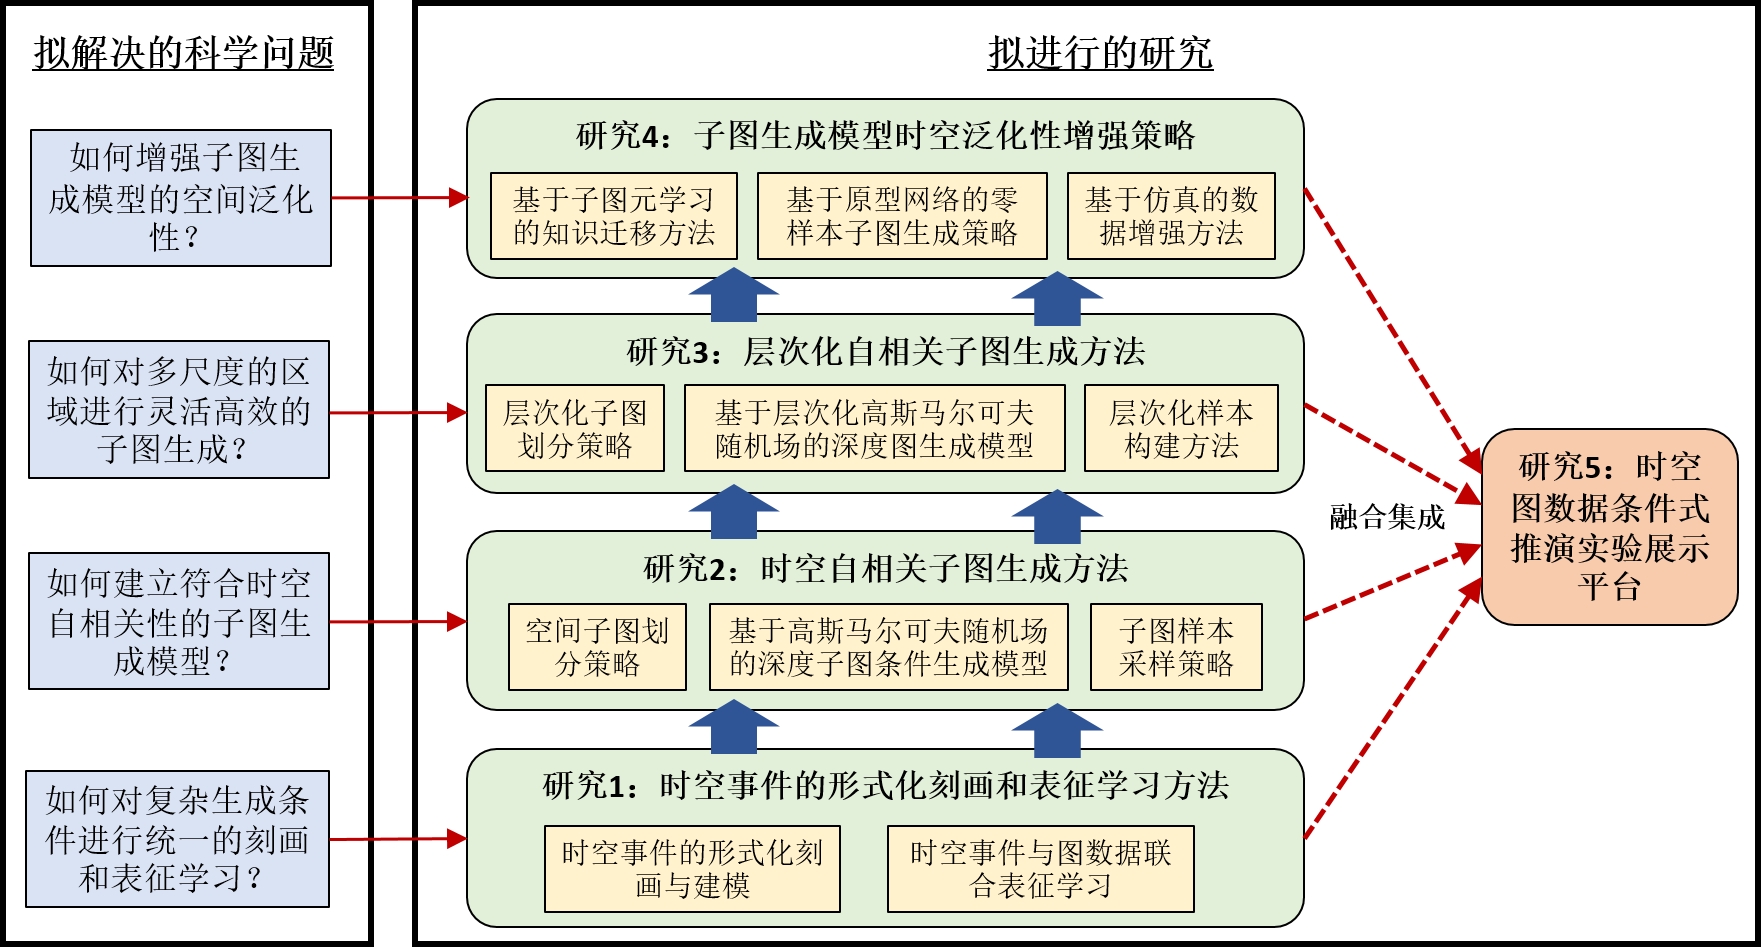
\includegraphics[width=1\linewidth]{fig/overall.png}
    \caption{本课题整体研究思路及各子问题关系}
    \label{fig:overall}
\end{figure}

\subsubsection{2.2.1 时空事件的形式化刻画与表征学习。}

我们首先对本课题中涉及的各输入变量进行形式化刻画,并给出关于时空图数据条件式推演问题的一个一般性定义。本问题的输入包括一个有向时空图$\mathcal{G}$ = $(\mathcal{V}, \mathcal{E}, \mathbf{X}, \mathbf{E})$, $\mathcal{V}$为$\mathcal{G}$中所有$N$个节点集合,$\mathcal{E} \subseteq \mathcal{V}\times \mathcal{V}$ 为所有有向边,$\mathcal{A_G}\in \mathbb{R}^{N\times N}$为图$\mathcal{G}$的邻接矩阵。每个节点$v\in \mathcal{V}$上还有其空间属性$v.o$,例如路段的形状等,用一个长度不超过$k$的二维坐标对序列$(x_1, y_1),(x_2, y_2)...(x_k, y_k)$表示。
$T$为时间区间,$T = \{1,2,3,...,t_{|T|}\}$。$\mathbf{X} \in \mathbb{R}^{N\times|T|\times d_X}$为节上非时空属性张量(例如交通流量、水流速度等), 其中$d_X$为图结点的属性维度。

%到在未来数据的概率分布,即${f_\theta}=p({\mathcal{G}_C}|\mathcal{G}, C,X_\mathcal{G})$,并通过对概率的采样生成新的数据$\hat{X}_\mathcal{G}$。

\begin{figure}
\centering
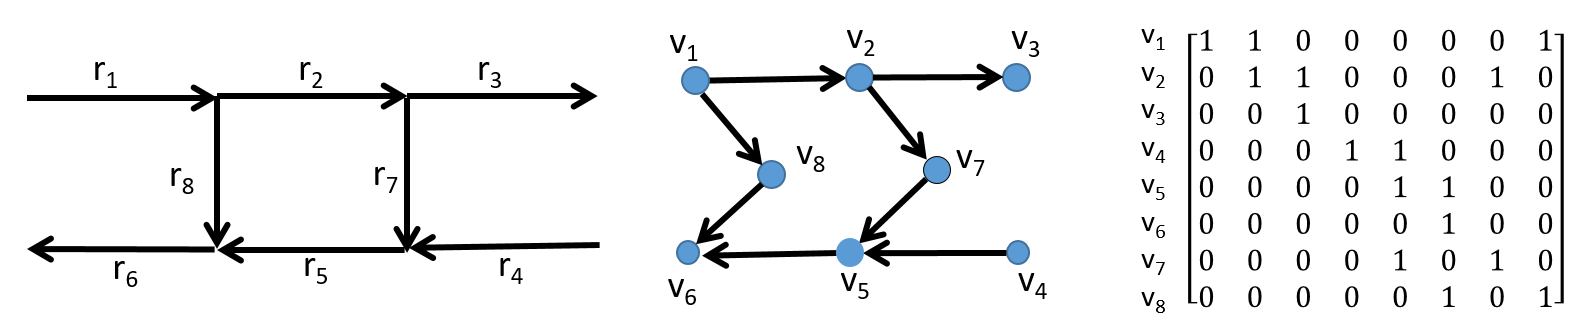
\includegraphics[width=0.95\textwidth]{fig/road_graph_1.png}    
\caption{{\kaishu 基于有向属性图的交通网络表示示例。左:路网结构;中:有向图表示,节点表示路段;右:相应的邻接矩阵。}}
\label{fig:graph-1-a}
\end{figure}

例如,在交通流量推演的问题中,可以将路网表示为一个有向图,每条路段定义为图节点,将道路之间的邻接关系定义为有向边。每个路段的信息包括空间几何属性,即$v.o$,例如形状;同时,节点还包含非时空属性$X$,例如车流量、最大车速、车道数量等。图~\ref{fig:graph-1-a}展示了时空属性图的一种表示方法,其中8个路段$r_i$可以表示为8个图节点$v_i$,并且根据邻接关系我们可以获得右侧展示的$8\times8$的邻接矩阵。在本课题中,我们假设时空图的结构固定,不随时间变化。%,并且不失一般性地,我们只考虑一维的目标变量生成问题,即只对$d_X$中的某一个维度的数据进行生成。

\textbf{问题定义:}假设推演的时间窗口长度为$l$,给定含有时空信息的事件集合$C = \{c_i\}$和时空图$\mathcal{G}$的一个子图$\mathcal{G}_g\subseteq\mathcal{G}$(包括相关的属性值),时空图数据条件式推演的目标是获取当$C$在$T$时刻发生时,$T+1$到$T+L$时间内$\mathcal{G}_g$上目标属性的分布概率,记为为$p(\mathcal{G}_g|\mathcal{G}_{g(T)}, C)$。%\xz{check}

\textbf{(1)时空事件的统一建模与形式化刻画}。首先,我们需要对事件$c$进行更明确的形式化刻画和建模。在时空图数据推演问题中,作为条件的时空事件种类繁多,例如交通事故、公共卫生管控政策、大型活动、道路建设、极端天气事件等。使用离散的事件类别标签既无法提供足够的信息来帮助时间推演,也会造成样本数据稀疏,因此需要对这些事件的时空及非时空信息进行建模和提取。然而,本问题中考虑的这些事件具有不同的时空维度。这使得对事件条件的建模和自动化信息提取存在困难。以交通事故为代表的点事件的位置信息只有一个坐标,即零维空间特征。交通管制涉及多条道路,其空间特征可理解为一维;而大型活动、道路建设等事件则影响一个区域,其空间足迹(spatial footprint)可以用二维的多边形代表。再考虑时间维度,各个事件的存在时间段各不相同,且空间足迹可能随时间有所变化,具有三维动态时空足迹。而需要进行推演的时空数据是图结构数据。这导致推演条件和推演目标数据融合困难。

另外,时空事件的非时空属性信息也不相同。一部分时空事件包含重要的非时空信息,例如大型活动的规模、人数等对交通流量影响很大的信息;极端天气事件的降水量信息也对河流水位变化推演至关重要。而另一些事件则很难获取定量的非时空属性,例如交通事故的信息往往涉及隐私,其对交通流量的影响也很难给出确定性的估计。在这种情况下,如何对事件进行统一建模则极具挑战。%目前的研究中,对时空事件的分析集中在检测(detection)和预报(forecasting)方面。在相关方法中,事件通常被提前假设具有一定的时空结构,并根据维度和类别分别研究。%例如交通事件可表示为路网上一个连通的子图、网格上的一个长方形区域、或者一个兴趣点(POI)集合。
%然而,在本问题中,事件的来源多样,时空维度不一,属性不一致。已有的表示方法不适用于本课题。

在本课题中,我们假设每个时空事件可以表示为一个多元组:$c_i = \{l^t_i, \mathbf{o^t_i}, \mathbf{a^t_i}\}$,其中$l^t_i$为事件存续的时间长度,$\mathbf{o^t_i}\in\mathbb{R}^{2\times k\times l^t_i}$为事件$i$的空间几何形状时间序列,每个时间$t$上都由不超过$k$个元素的二维坐标序列来表示。$\mathbf{a_i^t} \in \mathbb{R}^{l^t_i}$为表示事件强度的时间序列。在本问题中,为了表述的简洁性,我们仅考虑一维的量化属性来表示事件的强度。该事件强度可根据具体应用场景和事件的属性来定义。例如,在交通流量推演的应用中,造成路段无法通行的交通事故的强度可以设定为0,即对流量没有注入或消耗,而是单纯改变时空图的连通性;演唱会等大型聚集事件的强度可按照到达人数的时间分布,定义成值为负的时间序列,即从网络中吸纳的流量;相反,人群离场的大型事件则可定义为取值为正数的时间序列,表示向网络中注入的流量。相似地,在河水流速推演的应用中,降水事件的强度可表示为总降水量的时间序列,等等。图~\ref{fig:event1}给出了三种交通流量推演场景下事件的例子,其中下方的图为交通路段和事件的空间位置举例,上方的图为三个事件相应的强度序列。其中左侧图为路段$r_5$上发生的交通事故$c_1$,其强度为0且恒定不变;中间图为路段$r_3$,$r_4$,$r_7$附近发生的大型聚集活动,例如演唱会,其强度函数为负数序列;右侧图为同一地点的扩散事件,例如演唱会散场,其强度函数为正数序列。

\begin{figure}
\centering
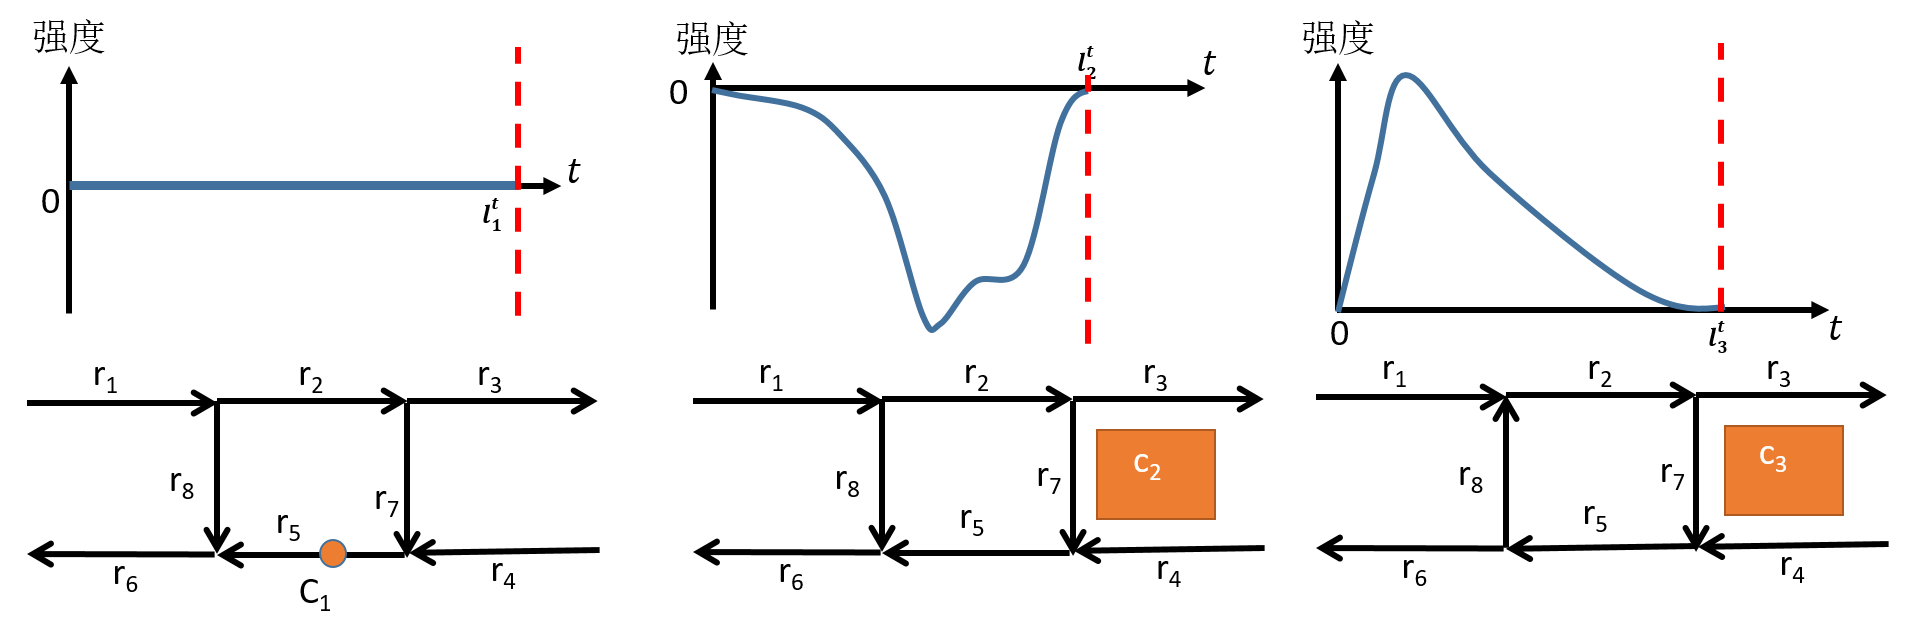
\includegraphics[width=0.95\textwidth]{fig/event-1.png}    
\caption{{\kaishu 交通流量推演场景下三种时空事件的举例。上方为相应的强度函数。}}
\label{fig:event1}
\end{figure}

本课题需要对时空事件进行双层次的建模,为后续表征学习提供信息。第一个层次是对时空数据的几何特征进行建模。如上文所述,我们用不超过$k$个二维坐标点表示每个时间片上事件的几何形状。第二个层次是对时空数据的网络拓扑信息进行建模,将事件表示为图结构的一部分来刻画其对时空图上节点的影响。我们将在研究思路部分对该层次建模进行详细叙述。%针对事件规模及其对时空图结构上数据的影响构建事件的图嵌入模型。
%最终对这两类信息进行表征学习,以得到低维的、连续的事件表征向量。

\textbf{(2)时空事件与时空图数据的联合表征学习}。时空事件的表征学习也是本课题的重要步骤之一。具体地,我们需要研究如何对事件进行信息提取,并生成一个嵌入表征向量。当需要对时空图数据进行条件生成时,可以将作为条件的事件输入特征提取编码器(由深度神经网络实现),获取相应的嵌入信息,再将嵌入信息结合需要生成地区的时空图数据来进行推演。

由于事件包含几何信息与图拓扑信息两个层次,其嵌入信息也应当由这两类嵌入信息联合得出。具体地,我们需要研究如何将事件的几何特征提取出来,并学习其对图节点上数据在欧氏距离空间上的影响。同时,我们还要提取出事件的图结构信息,并学习事件在图拓扑空间上对各个节点的影响。%例如,交通事故的影响如何通过路网结构传播从而对较远地区的产生影响。

基于上一章节中提出的事件建模与刻画方法,本课拟研究基于几何特征和图拓扑特征两个层面的事件联合表征学习框架。图~\ref{fig:embed}给出了对一个事件$c_i$进行特征提取的流程。首先,事件$c_i$的几何特征序列$o^t_i$将被提取出来,和时空图节点的几何信息(位置、形状等)一起被送入几何表征提取编码器。该编码器学习时空事件在欧式空间上(即对地理上临近的节点)影响的嵌入表示$z_{co}$。其次,事件$c_i$的图拓扑特征(基于2.2.1中的研究)将被提取出来,和时空图的拓扑信息(例如邻接矩阵)一起被提供给图表征提取编码器。该编码器学习时空事件在图拓扑空间上(例如,通过路网扩散延伸)影响的嵌入表示$z_{cg}$。最终,将事件几何时空表征$z_{co}$与事件图时空表征$z_{cg}$拼接得到事件-图联合表征$z_{c}$。

为实现上述框架,我们需要训练一个对事件进行几何信息提取的参数化编码器和一个对事件进行图拓扑信息提取的参数化编码器。本课题将具体研究如何通过深度神经网络实现这两个编码器,以及如何利用时空属性图数据进行训练来学习到这两个参数化的编码器。
\begin{figure}[t]
\centering
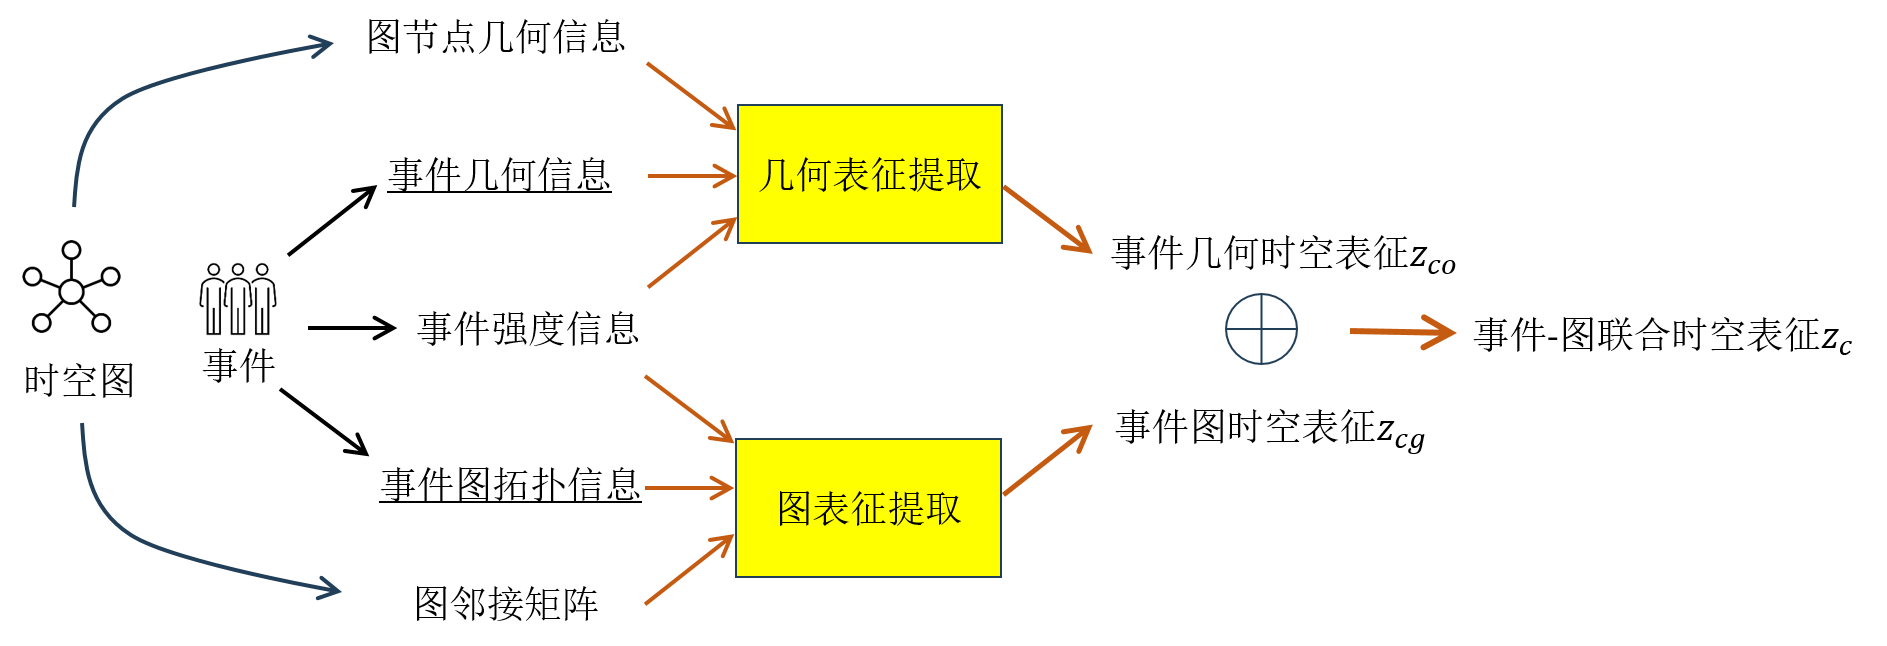
\includegraphics[width=0.99\textwidth]{fig/event_embedding-new.png}    
\caption{{\kaishu 事件-图联合表征提取的流程。}}
\label{fig:embed}
\end{figure}
%
%(1)时空事件的空间几何建模。时空事件可以表示为一个二维封闭的形状\footnote{本课题研究中暂不考虑形状嵌套、非欧几何空间形状等假设,只针对简单的封闭几何形状。},即一个经纬度坐标序列。与自然语言的表示方法相似,空间形状的坐标序列可以定义为一个二维的数值序列。%,并添加一个结束符号。需要指出的是,多边形的表示方法应该与序列起始点无关。
%对于零维的点数据,我们可以将自然地表示为一个坐标对(长度为1)。对于非闭合的线段,则可以从一端开始,将折线上的路径点表示为序列。例如,图~\cite{}中的路段集合可以表示为。$L = \{(x_1, y_1), (x_2, y_2), ...(x_n, y_n)\}$。
%
%对于普通的二维多边形的表示方法则稍显复杂。需要指出的是,多边形的表示方法应该与序列起始点无关。例如,一个由$n$个端点、$n$条边组成的多边形可以表示为:$O = \{(x_1, y_1), (x_2, y_2), ...(x_n, y_n), (x_1, y_1)\}$,也可以表示为$O = \{(x_n, y_n), (x_{n-1}, y_{n-1}), ...(x_1, y_1), (x_n, y_n)\}$。二者的表征向量应该相同。
%
% (2)时空事件的图拓扑属性进行建模。每个时空事件对临近图节点和边上的数据分布具有不同的影响。申请人提出将时空事件表示为对已有时空图结构的``编辑''操作这一新思路。具体地,我们将时空事件作为一个虚拟节点加入到已经定义的时空属性图中。根据不同类型的事件,我们可以定义三种图编辑的操作。
%
% 1)子图``删除''操作。当事件的时空范围直接涵盖一个或多个节点时,我们定义该事件为\\
% 2)子图``添加''操作。当事件的时空范围不直接与图节点重叠,但对空间上邻近的图节点产生``影响''时,可将该事件等价于在图中添加一个新的虚拟节点。根据空间范围查询可以获取该事件与哪些临近节点可能产生关联,进而添加这些节点与虚拟节点间的虚拟有向边。
% 3) 子图属性``修改''操作。
%
% 我们将输入定义为一个有向时空图结构$\mathcal{G_T} = \mathcal{G}\times T$,$\mathcal{G}$ = $(\mathcal{V}, \mathcal{E}, F, E)$, $\mathcal{V}$为$\mathcal{G}$中所有$N$个节点集合,$\mathcal{E} \subseteq \mathcal{V}\times \mathcal{V}$ 为所有有向边,$\mathcal{A_G}\in \mathbb{R}^{N\times N}$为图$\mathcal{G}$的邻接矩阵。
% $T$为时间区间,$T = \{1,2,3,...,t_m\}$
%         \item 节点属性张量$F \in \mathbb{R}^{N\times|T|\times d_V}$, $d_V$为图结点的属性维度。
%
% 时空数据的生成问题可以概括地定义为:
% \begin{itemized}
%     \item 给定:
%     \begin{enumerate}
%         \item 一个有向时空图结构$\mathcal{G}$ = $(\mathcal{V}, \mathcal{E}, F, E)$, $\mathcal{V}$为$\mathcal{G}$中所有$N$个节点集合,$\mathcal{E} \subseteq \mathcal{V}\times \mathcal{V}$ 为所有有向边,$\mathcal{A_G}\in \mathbb{R}^{N\times N}$为图$\mathcal{G}$的邻接矩阵。
%         \item 等间隔时间区间$T = \{1,2,3,...,t_m\}$
%         \item 节点属性张量$F \in \mathbb{R}^{N\times|T|\times d_V}$, $d_V$为图结点的属性维度。
%         \item 生成条件$\mathbf{C} \in \mathbb{R}^{|\mathcal{V}|\times|T|\times d_C}$,$d_V$和$d_C$分别表示图结点的属性维度和生成条件维度
%     \end{enumerate}
% %$\mathcal{F_E} \in$ $\mathbb{R}^{|\mathcal{E}|\times|T|\times d_E}$, 
%     \item 要求:
%         \begin{enumerate}
%         \item 参数化生成模型$\mathcal{F_\theta}: (z, \mathbf{C}) \rightarrow \hat{D_V}$,使得$\mathcal{F_\theta}$生成的数据$\hat{D_V}$符合真实数据在$\mathbf{C}$下的分布。
%     \end{enumerate}
% \end{itemized}
%
%
%
%
%同时,事件对周边环境具有复杂的影响,其中既有地理空间上的影响(例如公共卫生管控政策影响其覆盖地区出行需求),也有图拓扑结构上的影响(例如交通事故影响其附近路网的局部交通流量),如何对这些复杂影响进行表征学习也是实现图数据推演的重要技术基础。因此,本课题拟研究时空事件的统一化建模和表征学习。具体研究包括:
%
\subsubsection{2.2.2 自相关的时空子图生成学习策略}
时空图的生成学习面临的一个首要问题就是图的生成方式。根据1.2章节中对国内外研究现状的分析,已有的图数据生成方法,无论是一次性生成还是顺序生成,都假设算法的生成目标是一张语义、结构完整、独立的图,训练数据集中的样本已经给定,如何构建则不需要单独研究。然而,这些方式在时空图数据上都有很大不合理性。首先,本课题中研究的时空图的规模决定了整图生成并不现实。对大规模的图数据进行整图生成训练,对计算资源的要求巨大。而且,训练一次性整图生成模型将使得每个时间点上只有一个训练样本,造成训练数据的稀疏,使模型难以训练。因此,本问题中的图生成方式只能采取非整图生成的模式。另一部分已有的图生成技术采取了顺序生成的方式,即将一个图的生成任务分解为对节点或边的顺序生成,依据随机游走,广度优先序列等方法将图数据降维成一维序列。然而,此类生成方式对时空属性图也不适用。时空有向图各部分之间的空间依赖性通常是非偏序关系,每个节点、子图上的数据分布都与周围邻接的节点、子图相关。序列化生成是对邻接关系的降维,会造成结果依赖于生成顺序。同时,在规模较大的时空图上,序列生成的步骤较多,会造成误差的积累,影响生成质量。

故而,本课题采取与以上策略不同的生成策略。一种逻辑上合理可行的方法是局部子图生成,即将输入的时空图划分为若干个子图,并以这些图上的数据作为样本,学习一个对子图的生成模型。最后,当进行数据推演时,对各个子图上的数据进行生成并将结果拼接组合起来,生成出最终结果。

实现上述子图生成方式有三个关键的技术挑战。\textbf{首先,子图的定义并没有一个标准化的规则}。不同应用场景下的子图代表不同意义,其划分的物理含义也不同(例如街区、城镇、水系等)。有些场景下时空图并无明确的子图结构定义。因此,需要根据数据对子图进行合理的人为划分。%\textbf{其次,如何在已划分的子图上进行训练数据的采样是一个重要问题}。不同于已有的图生成方法,本问题的训练数据集并非已经提供好的图样本集合,而是需要从输入的时空图里进行采样来获得。根据时空事件在图中的分布,我们需要对事件周边时空区域进行有策略的采样,以保证训练样本能够准确代表子图内和子图间的数据分布依赖关系。
\textbf{其次,自相关的子图生成假设不同于现有的深度学习模型}。已有的图生成技术通常假设所有的样本图都是来自于同一个隐变量空间的独立随机样本。模型学习如何将采样自这个隐变量空间的随机隐变量映射到对应的图结构上。而在本课题中,由于时空图的特性,这一基本假设并不成立。由于所有子图都来源于同一个时空图的不同区域,临近的子图之间天然地存在时空自相关性,其数据分布特性并非是独立的。如果对其进行独立生成则会造成子图之间数据的不连续性,严重影响生成质量。\textbf{最后,自相关子图生成并没有一个标准的样本数据集可用},而是需要重新构建。

基于以上挑战,本课题将对以下三个关键问题进行深入研究,最终提出完整的基于子图生成的时空图数据生成策略。

\textbf{(1)时空子图划分策略}。
%当模型训练完毕后,对给定的目标区域进数据生成的策略也是需要研究的重要问题。在本课题中,推演任务需要生成的区域由用户给出,大小并不固定。理论上,我们可以对区域内所有大小为$N_{max}$的子图(包含有重叠的子图)进行生成并对结果进行平均。然而,这样的生成方法会带来巨大的计算开销。如何对该区域进行子图划分并进行数据生成将影响推演的计算效率和生成数据的准确性。
对子图的划分可以独立于模型训练进行。形式化地,给定一个时空图$\mathcal{G}$, %$\mathcal{G}_g\subseteq \mathcal{G}$作为生成范围,$N_{max}\leq|\mathcal{G}_g|\leq|\mathcal{G}|$,
划分策略的目的是给出$\mathcal{G}$的一个划分方案$P_{\mathcal{G}}=\{\mathcal{G}^1_P, \mathcal{G}^2_P, ..., \mathcal{G}^k_P\}$, 将$\mathcal{G}$划分为$k$个节点数为$N_{max}$的可重叠的连通子图,使得$\mathcal{G} = \bigcup_{i=1}^k\mathcal{G}^i_P$。图~\ref{fig:part_1}展示了一种在10个节点有向图上的子图划分策略,将其划分为3-节点子图,右边是其对应的超图表示。
\begin{figure}
    \centering
    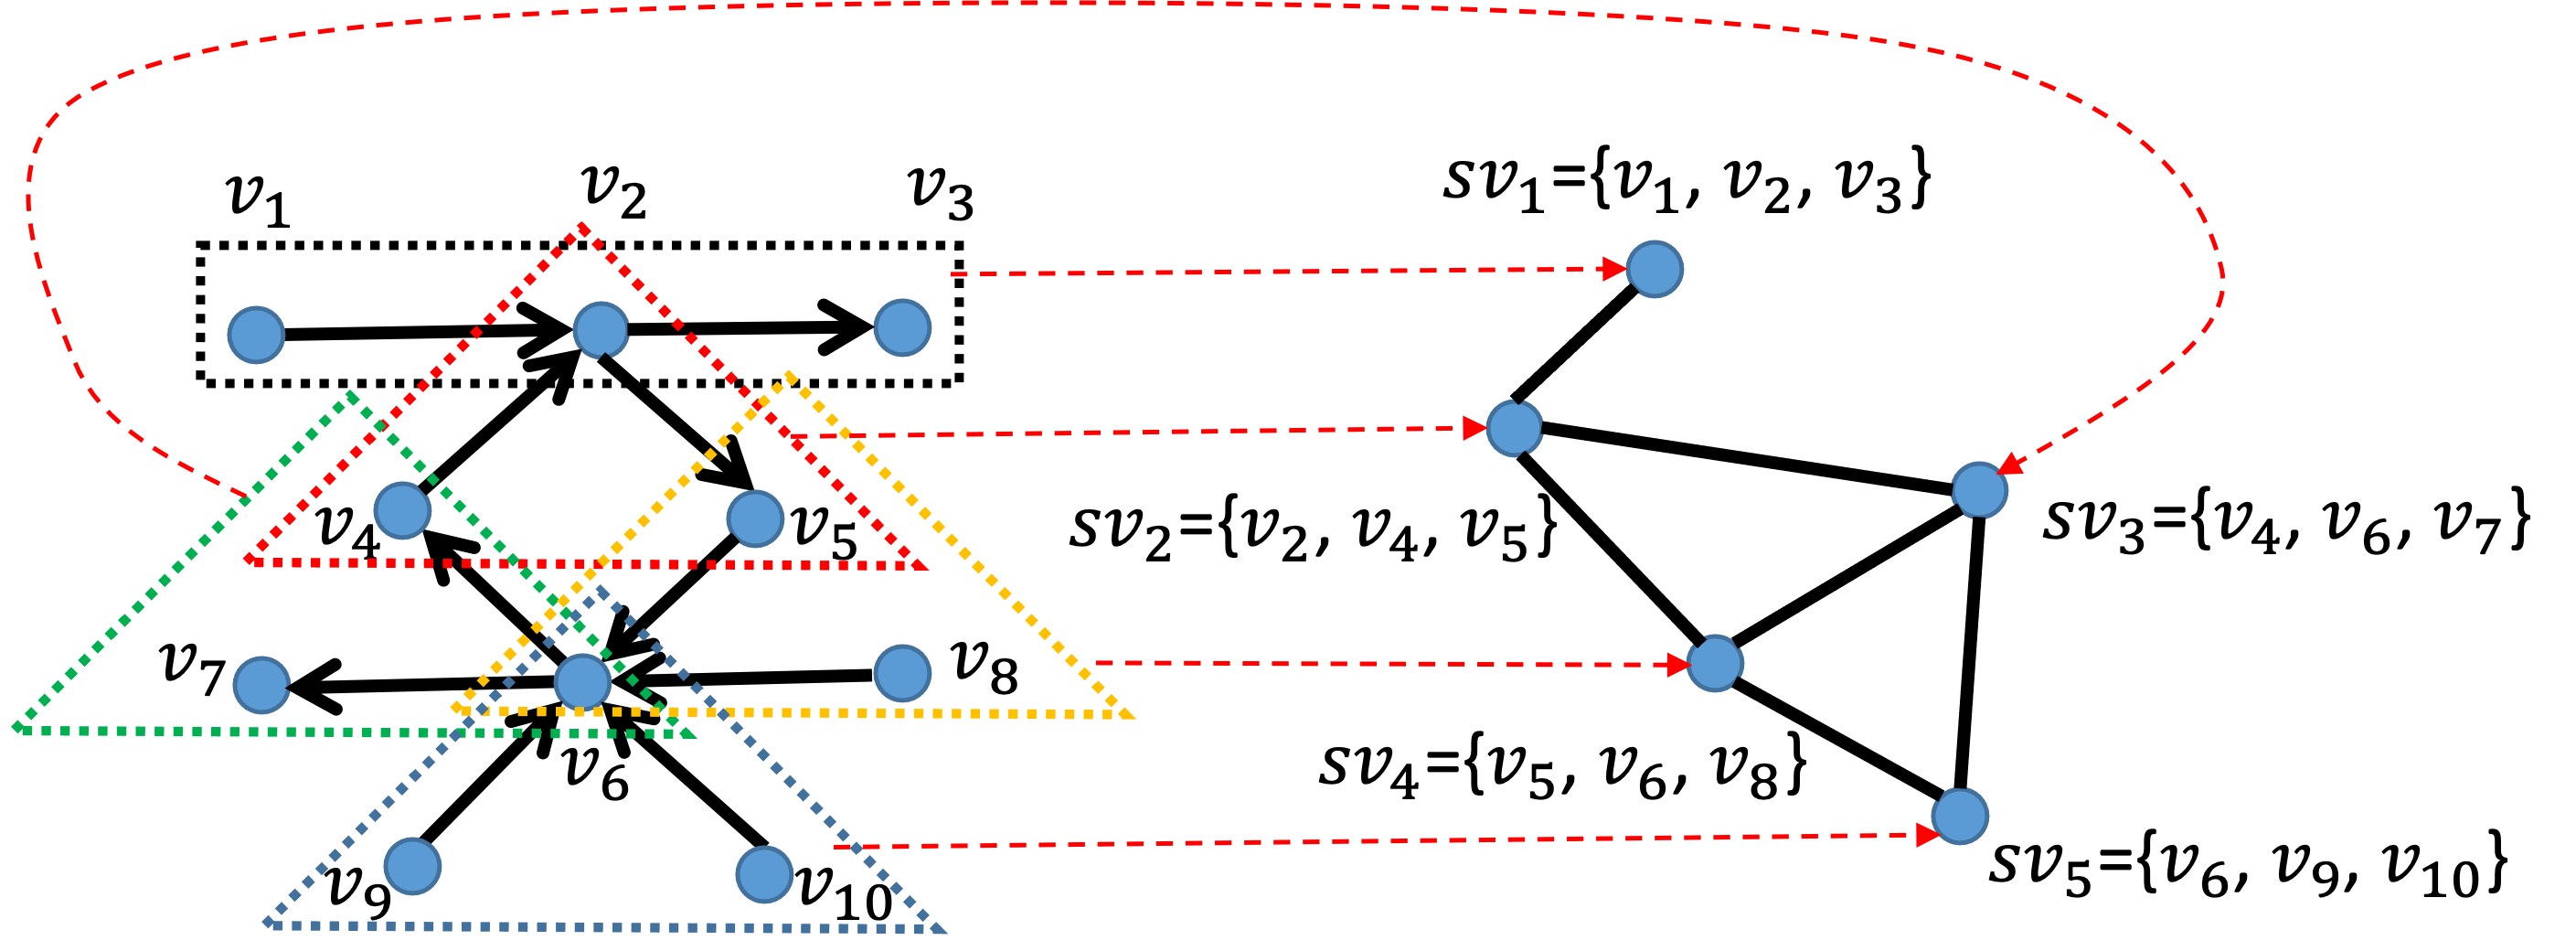
\includegraphics[width=0.8\linewidth]{fig/paritition-1_new.png}
    \caption{一种子图划分策略示例}
    \label{fig:part_1}
\end{figure}
%由于子图中需要尽可能地包含节点间的互相依赖信息,我们规定每条边$e\in \mathcal{E}$必须包含在至少一个子图内。
当划分完成后,我们可以将每个子图表示为一个超节点,并为临近或有交集的子图对应的超节点之间建立一条超边,从而将原始时空图转化成为一个无向超图。在训练阶段,算法对生成条件时空影响范围内的子图进行采样,获得训练样本。当模型训练完成之后,模型通过对$\mathcal{G}^i_P$上的数据生成完成推演任务。时空图划分需要遵循两个目标,第一是提高子图内部数据的相关性,降低不同子图间数据的相关性。这样做的目的是降低子图间的依赖关系,使得生成模型更容易生成出合理的数据分布。第二是尽量减少子图之间的重叠,减少数据的重复生成。

本问题的难点在于(1)如何定义一个合适的目标函数来评价划分的优劣程度,(2)如何设计高效的算法,基于该评价函数进行子图划分。由于需要保证子图的连通性,本问题中的子图间可以重叠。故而,该子图划分问题不同于组合优化中常见的图划分或者节点覆盖问题。同时,由于需要考虑节点属性的历史相关性,所以单纯基于图结构的划分方法也不适用,需要设计一个新的聚类算法来解决该问题。\textbf{本课题将对划分方法进行具体研究}。

% \textbf{(2)基于空间图采样的学习样本生成策略}。

% 针对每一个时空事件,我们需要在其影响的时空范围内对数据进行采样,从输入的时空图中选取若干个子图,收集事件前后的子图数据并组成一对时空图作为训练样本来训练模型。这里一个关键的问题是用怎样的策略来选择对哪些子图进行采样来构建训练样本。例如,可以采用等概率采样的方法,对每个事件附近一定时空范围内的子图进行等概率采样。显然,这种策略无法帮助模型学习到临近子图数据上的时空依赖性。相反地,子图采样需要尽可能地将相关性大的子图样本采集到训练集中帮助模型的训练。本课题计划采用循环更新采样概率的方法对子图进行重要性采样(importance sampling),并针对图结构数据使用自相关性度量函数来指导采样概率的更新,使得采样过程能够既收集到各个子图内部数据分布信息,又能够采集到足够多的临近子图样本,为后续自相关的子图生成模型训练奠定基础。

\textbf{(2)基于自相关性隐变量空间的子图生成模型}。
生成模型的设计是本课题的核心。在对子图进行划分后,我们需要设计对子图数据进行生成式学习的模型以及相应的算法。常见的生成模型包括图变分自编码器(G-VAE),条件对抗生成网络(cGAN),降噪扩散随机模型(denoising diffusion probabilistic model)等。其核心思想是学习一个解码器$g_\theta$将一个随机噪声向量$z$映射到实际数据上。针对$z$如何获取,模型采用的方法各不相同,例如GraphVAE通过一个编码器函数$f(G)$计算出$z$变量的分布参数$\mu$和$\sigma$来拟合隐变量先验分布$p(z)$,再用解码器将采样的$z$映射回数据空间。基于GAN的模型则没有编码器,而是由用户给出或通过一个推断网络计算出$z$的取值并由解码器映射回数据空间,依靠一个判别器来进行反馈。而diffusion model则是学习如何通过加噪声的方法将编码后的数据样本映射到一个简单的隐变量分布,例如标准正态分布上,再由其逆过程即减噪过程完成向数据空间的映射。

本课题的一个核心思想是假设$\mathcal{G}$上每一个子图的数据分布由一个自相关的空间随机过程$\Phi$生成\footnote{本课题中,子图上数据的时序自相关性由隐变量$z$控制,通过与历史数据和事件条件隐变量$z_c$共同解码来直接生成自相关的时间序列,故隐变量自相关模型中仅考虑空间的自相关性。}。所有子图样本对应的隐变量$z_1, z_2, ... z_M$的联合分布由$\Phi_S$给出,而非一个独立随机同分布的隐变量$z$,即$\mathbf{z}\sim\Phi$。%形式化地,$p(z^1_S, z^2_S, ... z^M_S)\sim \Phi_S(\mathbf{h}^1_S, \mathbf{h}^2_S, ... \mathbf{h}^M_S)$,其中$\mathbf{h}^1_S,\mathbf{h}^2_S ... \mathbf{h}^M_S$为所有子图的空间位置表征嵌入向量。当考虑事件$C$发生的条件时,上述概率可修改为$p(z^1_S, z^2_S, ... z^M_S|\mathccal{C})\sim \Phi_S(\mathbf{h}^1_S, \mathbf{h}^2_S, ... \mathbf{h}^M_S|%\mathbf{h}^1_c,\mathbf{h}^2_c,...,\mathbf{h}^w_c z^t_g)$, $z^t_g$为事件的联合表征向量(已在2.2.2章节中讨论)。
模型设计的核心目的是设计一个深度神经网络来完成子图样本和$\Phi$分布空间的互相映射。通过选取合适的随机过程$\Phi$的参数化表达来进行采样,最终完成对具有相关性子图的生成。具体地,本课题计划将子图隐变量定义为一个高斯马尔科夫随机场(GMRF),即符合马尔科夫独立性的多维高斯分布,由均值向量$\mathcbf{\mu}$和精度矩阵(即协方差矩阵的逆矩阵)$\mathbf{Q}$来刻画。马尔可夫独立性指每个图节点上的隐变量只依赖于其邻居节点的隐变量,而和其他节点上的隐变量无关。通常,GMRF需要满足无向图结构。基于之前阐述的子图划分的思路,我们将子图空间变换为无向超图,通过将子图隐变量定义在新的超节点上使问题符合这些条件。%同时,近年来的相关研究结果表明,GMRF的求解可以通过深度学习模型训练获得。
%本课题将基于图变分自编码器GraphVAE的架构,设计相应的编码器函数对GMRF分布进行拟合,以及解码器函数来将采样后的隐变量映射回图数据空间。同时,本课题还将对具体的理论进行分析,验证其统计上的合理性。
\textbf{本课题将对如何设计、实现这一自相关性子图生成模型进行深入研究}。

\textbf{(3)自相关子图样本构建和采样策略。}不同于整图生成问题中,图样本均为已经准备好的独立数据样本,本问题中的训练子图样本需要从整个时空图上提取并构建成训练样本。由于自相关的子图生成需要对子图间的依赖关系进行学习,常见的独立样本采样方法不适用于本问题,需要研究新的采样策略来帮助模型学习重要知识。同时,由于事件条件的稀疏性,我们需要将事件与子图匹配并选取有价值的样本送入模型继续进行训练。\textbf{本课题将对如何高效进行模型训练和数据生成进行具体研究}。

% \textbf{(1)基于空间图采样的学习样本生成策略}。

%相应地,有两种较为合理的生成方式。第一种是局部生成,
 %在这种局部生成模式下,第一个需要解决的问题是如何构建子图训练数据。针对每一个时空事件,我们需要在其影响的时空范围内对数据进行采样,从输入的时空图中选取若干个大小固定的子图,收集事件前后的子图数据并组成一对时空图作为训练样本来训练模型。这里一个关键的问题是用怎样的策略来选择对哪些子图进行采样来构建训练样本。例如,可以采用等概率采样的方法,对每个事件附近一定时空范围内的子图进行等概率采样。显然,这种策略无法帮助模型学习到临近子图数据上的时空依赖性。相反地,子图采样需要尽可能地将相关性大的子图样本采集到训练集中帮助模型的训练。本课题计划采用循环更新采样概率的方法对子图进行重要性采样(importance sampling),并针对图结构数据使用自相关性度量函数来指导采样概率的更新,使得采样过程能够既收集到各个子图内部数据分布信息,又能够采集到足够多的临近子图样本,为后续自相关的子图生成模型训练奠定基础。

\subsubsection{2.2.3 层次化自相关子图生成学习方法}

%当时空推演任务的生成区域较大,包含的子图较多时,对2.2.3中提出的高斯马尔科夫随机场进行采样面临计算开销大的挑战。
很多时空图都具有层次化结构,例如交通网络中,不同城市、地区、街道、社区之间的交通流量构成了路网结构的不同层次;河流水网中,支流向干流汇入也构成一个层次化结构。针对具有层次结构的时空图,我们也可以用层次化的子图生成方式来进行推演。层次化生成是指对时空图进行多层次的子图划分,逐层将子图聚合成上一层图中的超节点(super-node),得到一系列不同尺度的超图(super-graph)。在进行数据生成时,则根据层次的顺序逐渐对需要生成的区域进行更细粒度的生成。层次化生成的优点是能够提供多尺度的数据生成,尤其在局部尺度范围数据生成时具有更好的效率。下面介绍本研究项的各个具体任务。%但是该任务需要学习不同层次图结构之间的生成方法,故而具有与2.2.3中的子图生成方法具有不同的挑战。

\textbf{(1)时空图的层次化划分方法:} 给定一个时空图结构$\mathcal{G}$,我们可以定义一个层次化划分结构$\mathcal{H}:\{\mathcal{G}^1,\mathcal{G}^2,...,\mathcal{G}^L \}$,其中$L$为划分的层数,$\mathcal{G}^i$为第$i$层的图结构,$\mathcal{G}^L = \mathcal{G}$。$\mathcal{G}^i$的每个节点对应$\mathcal{G}^{i+1}$的一个子图,即超节点。$\mathcal{G}^i$中的每条边$\mathcal{E}^i_{u,v}$表示节点$u^i$与$v^i$之间的连通关系。%,即$\mathcal{G}_{i+1}$中两个子图之间的总体连通关系。
每个层次图$\mathcal{G}^i$的节点属性可表示为该节点对应的区域中属性的一个整体统计值(例如总交通流量,平均车速度等)。层次化生成需要训练一个生成模型,从上至下沿着$\mathcal{H}$的层次,顺序地对$\mathcal{G}^i$上的数据进行生成,最终完成对$\mathcal{G}$上数据的生成任务。相应地,本课题首先需要研究如何建立层次化的子图划分。我们限定每个子图(即超节点)大小不超过$N_{max}$,通过自底向上的层次化聚类得到一个在给定的时空图$G$上的划分方案$\mathcal{H}$。章节2.2.3中研究的子图划分问题可以看成是层次化子图划分的第一步,即从$\mathcal{G}^L$到$\mathcal{G}^{L-1}$的划分。基于2.2.3中提出的划分办法,$\mathcal{G}^{L-1}$层以及更高的层级中的子图均为无向图。%由于图连通性的要求,每一层的子图之间有可能会出现重叠。我们定义两个$\mathcal{G}^i$的超节点$u^i$与$v^i$之间有一条无向边$\mathcal{E}^i_{u,v}$,当且仅当$u^i$与$v^i$在$\mathcal{G}^{i+1}$上对应的子图有交集。
图~\ref{fig:part-2}给出了一种层次化子图划分的方案,其中$L=3$,$N_{max} = 3$。

与2.2.2中探讨的问题类似,本问题中,我们的目的是尽量将相似度高的第$i$层子图节点划分进同一个子图,从而使其属于第$i-1$层的同一个超节点。子图相似性的度量需要考虑三个方面,即历史数据分布的相关性、图结构的连通性以及地理空间的临近性。同时,类似于2.2.2中阐述的划分原则,由于图连通性的要求,每一层的子图之间有可能会出现重叠,但要尽量减少子图之间的重叠以减少对数据的重复生成和时空关系的复杂依赖结构。\textbf{本课题将对层次化子图划分的方法进行详细研究}。

\begin{figure}
\centering
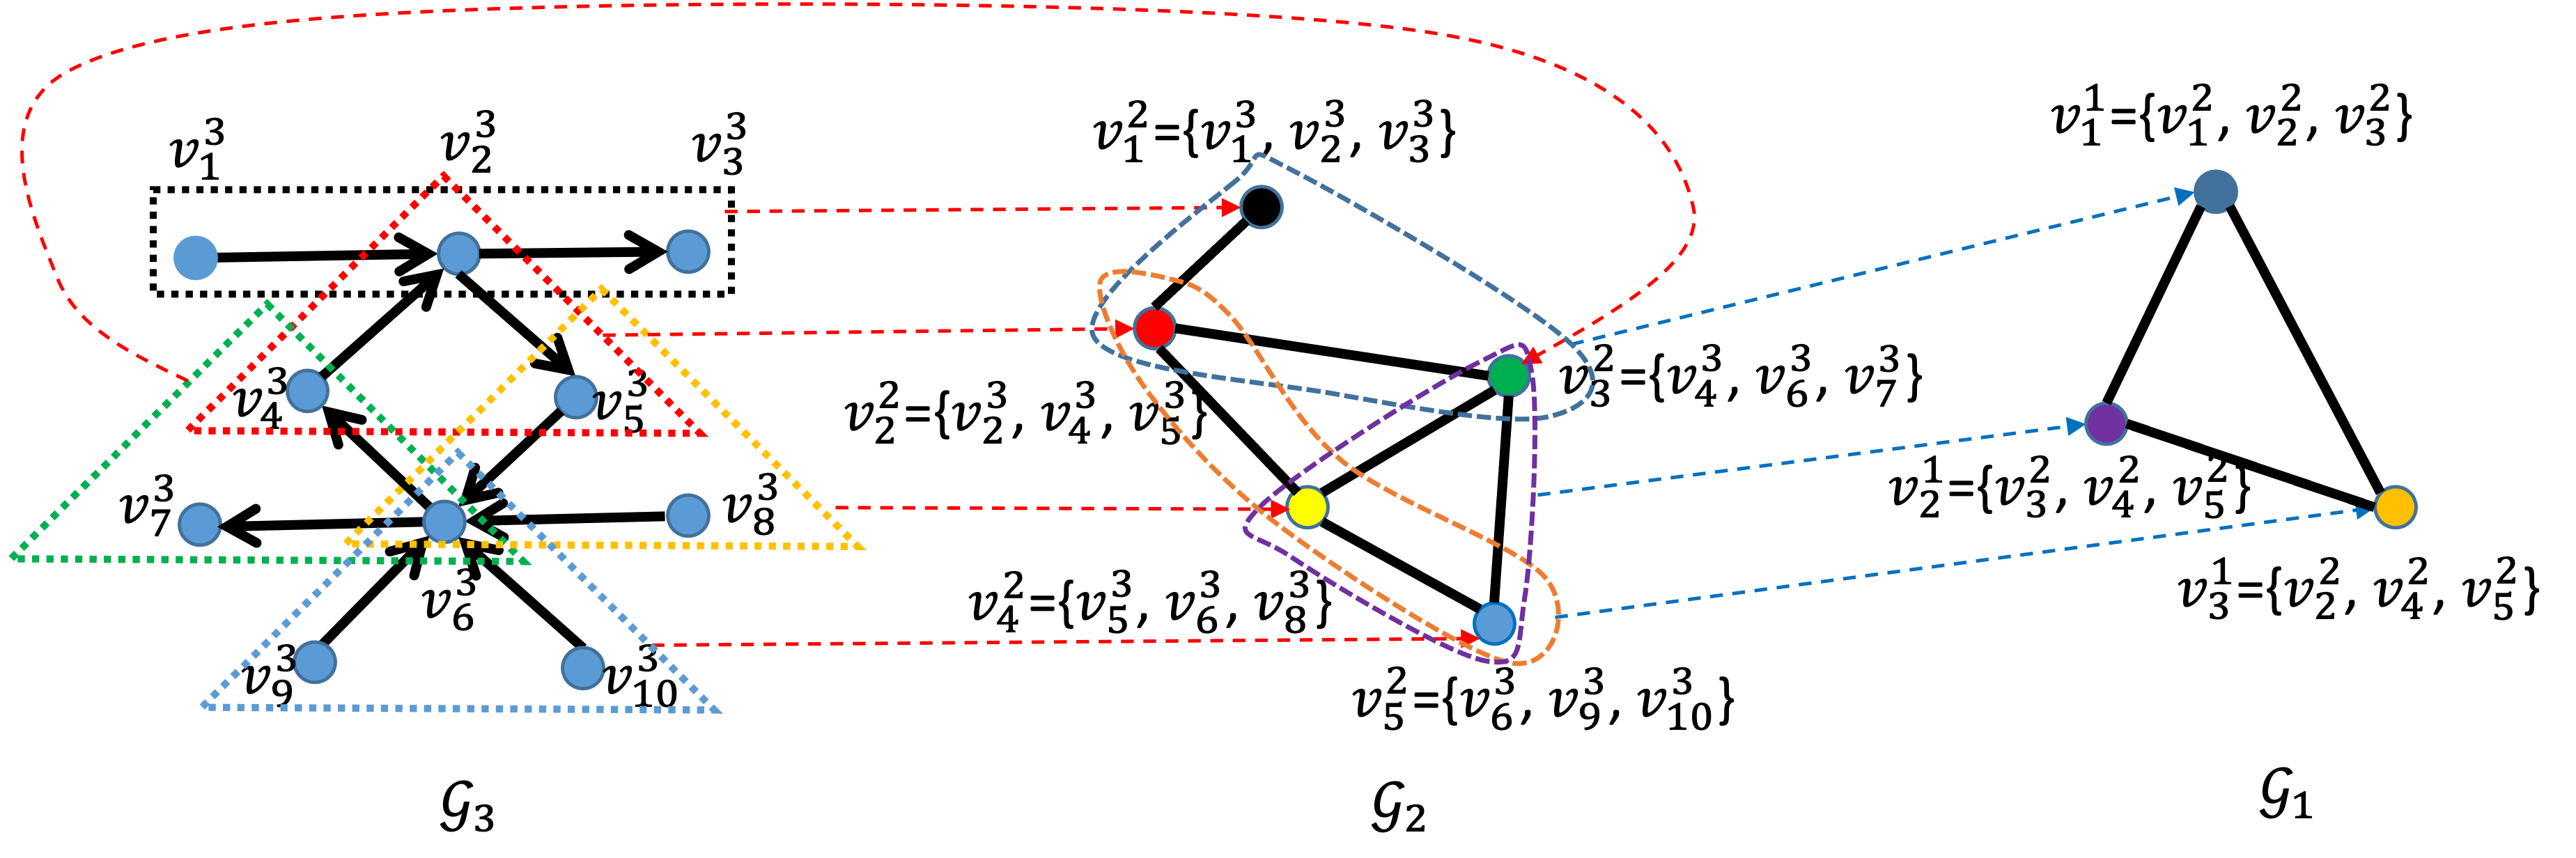
\includegraphics[width=0.99\textwidth]{fig/paritition-2_new.png}    
\caption{{\kaishu 一种层次化子图划分方案的举例}}
\label{fig:part-2}
\end{figure}


\textbf{(2)时空子图的层次化生成学习模型与算法:}在建立了层次化划分方案后,我们需要研究如何学习一个层次化的时空图数据生成模型。%生成一个完整时空图的概率为$p(\mathcal{G} = \mathcal{G}_L)$,即最底层图的生成概率。
在这一子问题中,本课题拟扩展2.2.2中提出的基于高斯马尔科夫随机场(GMRF)的子图生成模型,将不同层次的子图数据分布映射到一个层次化的高斯马尔科夫随机场上来解决生成问题。%层次化高斯马尔科夫随机场(Hierarchical Gaussian Markov Random Field)是对高斯马尔科夫随机场的扩展,其不但刻画同层节点间的自相关性,还刻画临近层级节点间的依赖性。
下面简单介绍本问题中使用的层次化马尔可夫随机场的概念、假设、以及具体的问题描述。

首先,在本问题中,我们对自相关性假设进行调整,将第$i$层的子图相关性结构分割为多个独立的维度更低的GMRF。具体地,第$i$层子图的隐变量$z^i$的分布将由其所属的第$i-1$层超子图结构上定义的$N_{max}$维GMRF分布来决定,而非整个第$i-1$层超图上的GMRF。不同超子图之间的相关性则由更上层超子图上的GMRF来体现。例如,图~\ref{fig:part-2}中第二层超图$\mathcal{G}_2$上的子图$\{v^2_1, v^2_2, v^2_3\}$(蓝色虚线)上可定义一个3维GMRF。在第三层图$\mathcal{G}_3$上对应的三个子图$\{v^3_1, v^3_2, v^3_3\}$(黑色虚线),$\{v^3_2, v^3_4, v^3_5\}$(红色虚线),$\{v^3_4, v^3_6, v^3_7\}$(绿色虚线)的隐变量即服从这个3维GMRF。这样我们可以将局部数据生成的问题分解为多个更低维度的子问题,针对需要推演的区域进行数据生成,避免对整体GMRF的采样,以提高计算效率。

其次,我们需要对不同层次子图之间的相关性进行建模。理论上,每一层图数据的分布也同时依赖于其之前所有层的图结构,即$p(\mathcal{G}^i|\mathcal{G}^{i-1}, \mathcal{G}^{i-2},...,\mathcal{G}^{1})$。根据类似的层次化数据生成模型的常见做法,我们假设每个第$i$层的超子图$\mathcal{G}^i_j$上数据的分布概率仅依赖其父层超子图$\mathcal{G}^{i-1}_k$,而与其祖先层的图数据无关。我们称之为层间条件独立性假设。%即$p(\mathcal{G}_i|\mathcal{G}_{i-1}, \mathcal{G}_{i-2},...,\mathcal{G}_{1}) = p(\mathcal{G}_i|\mathcal{G}_{i-1})$。
基于这一假设,我们可以将2.2.2中提出的基于GMRF隐变量分布的模型架构进行扩展。和之前一样,每个超图上隐变量$z$服从标准GMRF分布,由均值向量$\bf{\mu}$和精度矩阵${Q}$来控制。在之前的GMRF定义中,我们指定一个参数已知的GMRF作为先验概率$p(z)$,并训练GraphVAE模型的编码器将输入映射到这个分布上。在层次化建模的假设下,第$i$层每个超图的$\mu$和$Q$的取值不再给定,而是根据上一层超图的数据来生成,即
\begin{equation}
    p(z^i) = \Phi(\mathbf{\mu}(\mathbf{\theta}), Q^{-1}(\mathbf{\theta})), \mathbf{\theta} = f(\mathcal{G}^{i-1})
\end{equation}
其中$f$为对上层超图进行编码的函数,用来获取超参数$\mathbf{\theta}$以便生成第$i-1$层每个子图中的$\mu$向量和$Q$矩阵。当生成每个超子图数据时,需要先获取其父层超子图上的数据,并生成相应的$\mu$和$Q$,继而对该超子图及其兄弟超子图(同属于一个父超子图的本层超子图)同时进行自相关的生成。

以上建模方式的优点在于,每个子图的生成仅仅依赖于其直系祖先超子图。根据层间条件独立性假设,我们可以对整个层次图进行层次化生成,并只针对需要推演的局部子图进行生成。例如,在图~\ref{fig:part-2}中,如果仅需要对$\mathcal{G}^3$中的$v^3_1, v^3_2, v^3_4$节点进行数据生成,则只需要先对第2层超子图$\{v^2_1, v^2_2, v^2_3\}$进行生成,再对$\{v^3_1, v^3_2, v^3_3\}$,$\{v^3_2, v^3_4, v^3_5\}$,$\{v^3_4, v^3_6, v^3_7\}$三个第3层子图进行生成即可,避免了对所有第3层子图的生成。\textbf{本课题将具体设计该层次化生成模型的架构,给出更为详细的理论基础,并提出训练算法}。

%在贝叶斯统计学习的相关研究中,GMRF的精度矩阵$Q$通常被假设服从一个威沙特分布(Whisher Distribution),由。相应地,我们修改GraphVAE的结构,通过

%由于前述的分析,生成一个完整的大规模时空图通常是不必要的,我们关注如何生成一个给定位置的第$L$层子图$\mathcal{G}^*_L\subseteq{\mathcal{G}_L}$。层次化生成的核心思想是,每个子图的数据分布只依赖于包含这个子图的上一层子图。由于每个子图可能被多个上一层子图覆盖,我们定义$\mathcal{G}^*_{i}$为第$i$层图中所有覆盖子图$\mathcal{G}^*_L$的子图集合。基于上述独立性的假设,每个子图的生成概率仅依赖于其之前层对应的超子图的生成概率。推广上述层间图的独立性假设,我们有$\mathcal{G}^*_L$的生成概率为$p(\mathcal{G}^*_L) = p(\mathcal{G}^*_L|\mathcal{G}^*_{L-1})\times p(\mathcal{G}^*_{L-1}|\mathcal{G}^*_{L-2})\times ... \times p(\mathcal{G}^*_2|\mathcal{G}^*_{1})\times p(\mathcal{G}^*_1)  = \prod_{i=2}^L p(\mathcal{G}^*_i|\mathcal{G}^*_{i-1})\times{p(\mathcal{G}^*_1)}$。由于第1层只有一个子图,即$\mathcal{G}_1$,故$p(\mathcal{G}^*_1)=p(\mathcal{G}_1)$。我们可以得出如下公式:
%\begin{equation}
% p(\mathcal{G}^*_L) =  \prod_{i=2}^L p(\mathcal{G}^*_i|\mathcal{G}^*_{i-1})\times{p(\mathcal{G}_1)}。
% \label{eq1}
% \end{equation}

% 将事件条件$C$考虑进来,则有如下公式\begin{equation}
% p(\mathcal{G}^*_L|C) = \prod_{i=2}^L p(\mathcal{G}^*_i|\mathcal{G}^*_{i-1}, C)\times p(\mathcal{G}_1|C)
% \label{eq2}
% \end{equation}

% 由此,该问题的核心是如何求解公式~\ref{eq2}中的两个条件概率,即给定事件条件下通过第$i-1$层子图来生成第$i$层子图集合$\mathcal{G}^*_i$的条件概率,以及最上层图$\mathcal{G}_1$在事件条件下的概率分布。本课题将对相应的模型和算法进行具体研究。
%$p(\mathcal{G}^*_L) = \int_z p(z_i)\times p(\mathcal{G}^*_L|z_i) dz$
%我们需要学习如何对一个第$L$层的子图$\mathcal{G}_L^j$进行数据生成。

%其次,本问题中的生成样本的构建是一个新的、复杂的问题。由于地理学第一定律和时空自相关性的约束,取自同一个时空图结构里的子图样本非独立样本。地理距离和拓扑距离越近的子图样本,其数据分布的相关性则越高。同时,由于时空数据的动态性,子图相关性强度难以具体量化描述。基于独立随机样本的图生成策略无法解决本课题中的生成学习需求。故而,本课题需要研究新的基于子图生成的时空图数据生成学习策略。
\textbf{(3)时空子图的层次化采样和训练策略:}对上述层次化生成模型进行训练时,我们还需要解决如何构建层次化子图训练样本的问题,以及如何对数据进行采样的问题。这里子图的构建和采样方法与2.2.2章节中的子图样本构建的方法相比有重要的区别。层次化生成中除了考虑每个子图与事件匹配,以及临近子图之间的共同采样方法外,还需要考虑如何对子图的父层、祖先层上的相关子图样本进行构建和采样,帮助模型学习到相关的层次化关联性信息。%例如,对事件$c$的影响范围内进行数据采样时,如果选中某个第$L$层子图$\mathcal{G}^*_L$,则需要同时对包含$\mathcal{G}^*_L$的所有层次的子图集合进行同步采样来帮助模型的学习。本课题将具体研究相应的采样算法和训练集构建的方法。
%同时,我们也需要考虑非兄弟但相邻的超子图间的相关性如何保证,以及在数据生成过程中,对属于不同子图重叠部分的重复生成问题。
\textbf{本课题将对层次化的采样的具体方法进行深入研究,并探讨高效的模型训练策略}。
%
%根据上述的层次化生成方式,每个子图的数据分布只依赖于其祖先层中包含该子图的
%例如,对图~\ref{fig:part-2}中第3层的子图$\{v_1, v_2, v_3\}$进行生成时,也需要考虑到与其重叠的子图$\{v_2, v_3, v_4\}$,以及其父层子图$\{v_1, v_2, v_3\}$的相关性问题。
%
%层次化采样的一个重要问题是如何针对每个事件条件的时空范围,选定合适的采样的尺度和层级。具体地,当一个事件发生时,我们需要对其影响范围内的不同层级的子图进行采样。
\subsubsection{2.2.4 子图生成模型空间泛化性增强策略}
%\textbf{首先},时空属性子图除了节点之间的拓扑关系,还包含重要的时空信息,包括位置坐标、几何形状信息等。以交通路网为例,如果用节点表示每个路段,用边表示两个路段是否邻接,则节点上的时空信息还包括用折线(Polyline)来表示的路段几何形状。此类信息对时空属性图上的数据生成非常重要,在对子图进行表征提取的时候,必须要考虑进去。\textbf{其次},时空事件例如工程建设、交通事故、交通管制等具有不同的时空范围、影响区域和类别属性。如果以离散标签的形式嵌入到生成条件中,则会造成数据样本稀疏,泛化性差。故而,需要对时空事件进行统一化建模,使其可以表示为连续的嵌入向量,从而在时空上具有更好的泛化性。\textbf{最后},如何将这两类表征向量进行时空对齐和匹配来作为生成条件,使得两者的时空关系能够被捕捉到。

本课题要解决的另一重要科学问题是如何增强子图生成模型的时空泛化性。根据地理学第二定律,变量间关系在时间和空间上的分布并不恒定,而是随时空环境而变化,即非同分布。这一规律也违反了目前经典的图数据生成模型对样本间同分布的假设。一个全局模型通常无法在所有时空位置上取得同样的表现。在异质性较强的时空图上,模型的泛化性有可能较差。例如,通过市中心商业区交通数据训练的生成模型,在对郊区工业区进行生成时可能会产生较大的误差,需要一个更准确的本地化模型。在本课题中,2.2.3章节介绍的层次化生成思路可以在一定程度上通过对不同区域训练不同的高斯马尔科夫随机场参数来解决这个问题,但是对事件样本稀疏的区域进行训练仍然是一个较大的挑战。在极端情况下,当某些区域没有事件样本时,模型无法学习到事件对时空图数据的影响。这造成了模型无法在这些地区进行准确推演。

针对这个重要且有挑战性的问题,本课题拟研究如何用元学习的策略通过不同区域之间的知识迁移来帮助事件稀疏地区学习到可用的子图生成模型。同时,针对无事件样本的情况,本课题还将探索如何用原型学习的方法增强模型泛化性,以及用基于仿真数据增强方法来帮助模型更好训练。下面详细介绍这几个拟研究的子问题。

\textbf{(1)基于子图元生成学习的知识迁移方法}。
%其次,由于事件在时间和空间上的稀疏性,很多需要推演的区域并没有足够的历史事件对模型进行训练,或没有发生过需要推演的事件类别。如何克服异质性挑战,增强模型的时空泛化性是一个重要课题。
%针对这个挑战,本课题提出两种解决思路。第一种是基于时空迁移学习的方法训练具有良好空间泛化性的模型。第二种是通过基于物理模型和基于代理人模拟的数据增强方法。
%
%常见的针对时空异质性的机器学习方法主要包括(1)以时空元学习为代表的知识迁移方法,(2)原型模型学习(prototype learning)等少样本学习策略,和(3)基于时空划分的时空集成学习。以上三种策略在时空图数据生成上均尚未被研究过。这三类方法各有优劣,提供了不同的技术选择。本课题拟对这三种技术路线分别进行研究,并设计相应的针对时空异质性的时空子图条件生成方法。
针对子图的时空异质性挑战,本课题拟研究时空图上的子图元生成方法来训练局部子图的生成模型。%另外,本课题拟研究基于代理人仿真的数据增强方法来增加训练集的空间覆盖度,帮助模型提高训练效果。
%
元学习(meta-learning)是一类迁移学习方法的总称。给定一系列具有关联性但不相同的任务$\mathcal{T}_i\in \mathcal{T}$,例如对包含不同种类动物组合的图片进行分类,元学习的目的是通过知识迁移学习,利用在部分训练任务上学习的知识,对没有见过的、样本较少的新测试任务进行快速适应和推断。元学习假设每个任务$\mathcal{T}_i$包含一个支持样本集(Support Set)$\mathcal{S}_i$和一个查询样本集(Query Set)${Q_i}$任务集合,所有任务$\mathcal{T}$服从一个特定分布,通过训练一个元模型$M_\theta$来学习这个任务分布的通用知识从而实现不同任务之间的模型迁移。在训练中通过采样不同的任务组合,我们可以用每个任务的支持集$\mathcal{S}_i$更新每个任务对应的具体模型$M_{\theta_i}$的参数$\theta_i$,并用这些任务的查询集来更新元模型$M_{\theta}$的参数$\theta$。经过上述训练步骤的多次迭代,得到一个具有良好泛化能力的元模型。每个任务的专用模型$M_{\theta_i}$可以由元模型$M_\theta$在对应任务的查询集上进行适应性优化后得到。

%时空元学习方法在非图结构的时空数据生成学习上已经被应用。例如,申请人团队前期工作中研究了基于时空元学习的跨城市栅格数据生成方法。通过学习一个元模型并将其微调后应用在不同的城市中,该方法可以成功地生成地理上具有异质性的移动数据分布热力图。
元学习是解决子图异质性挑战的一种有效合理的方法。通过训练一个具有良好时空泛化性的元子图生成模型和一个对元模型进行适应性微调的策略,我们可以通过少量训练样本获得针对时空图局部的本地化模型。目前的图数据上元学习方法主要针对不同的图分类任务间进行知识迁移(例如有环图、链式图、星型图等不同结构的标签预测)。然而,\textbf{在具有异质性的同一个时空图中进行不同局部之间的元生成学习,尚无已发表的成熟技术}。因此,本问题需要设计新的元学习算法来解决。

实现时空子图元生成学习需要解决\underline{两个独特的新问题}:(1)如何定义大小合适的生成任务。一个生成任务可能包括多个不同的子图,即子图群。一方面,为了减少本地模型的数量,降低模型训练的复杂度,我们希望尽量减少任务数量。另一方面,为了提高模型在各个任务上的表现,我们还希望将异质性较强的区域划分成不同的任务,单独训练不同模型来提高生成效果。如何对这两个冲突的目标进行平衡是一个挑战。由于时空异质性的结构通常难以准确、定量地刻画和描述,所以对空间进行预先划分并单独训练多个模型的方法并不可行。(2)如何根据空间分布对任务进行有策略地采样来充分让元模型获取可泛化的知识。这里,我们希望尽量采集到具有异质性的任务(例如空间上分散的子图生成任务)来增强元模型的泛化性,而避免过度采样同质化的任务。如何在模型训练中根据子图的时空属性和分布做到这一点,是一个新的技术挑战。\textbf{本课题将对这两个核心问题进行研究,并探索一种自适应任务划分的子图元学习方法和任务采样和模型训练方法}。

\textbf{(2)基于原型网络的少样本模型训练方法。}
另一种增强泛化性的方法是原型学习(Prototype Learning)。元型学习是一种少样本学习策略。通过训练,模型学习一系列的具有典型性的输入样本的特征,称之为原型(prototypes)。同时,模型学习如何度量一个输入样本与这些原型之间的相似度。当一类新样本被送入模型,模型可以通过比对输入样本和各原型之间的相似度来判断新任务与原有任务之间的相似度,并利用少量样本进行微调后建立输入输出之间的新关系。原型学习的基本假设是不同类别输入之间具有隐含的相似性,故而可以通过对其他类别输入输出关系的``借鉴''来进行模型推断。目前对原型学习方法的研究主要集中在分类问题上,尚无成熟的针对子图生成问题的原型学习方法。%\xz{check here}

\textbf{(3)基于场景仿真的数据增强方法。}除了采用机器学习方法外,本课题还将针对城市交通流量条件式推演这一具体场景进行数据增强来添加有效的训练样本。通过与交通领域的专家进行合作,本课题将针对典型交通事件影响下的交通流量进行基于代理人的模型仿真,来收集更多数据,以填补数据稀疏区域的样本空白。同时,新数据还可以用来交叉验证模型生成的推演结果的合理性。
%由于时空异质性的空间结构很难量化描述,所以具体应该对哪个局部进行任务采样是一个复杂问题。本课题中,我们需要训练一个全局的参数化子图生成模型$f_{\mathcal{\theta}}$,和一个本地化的模型$f^*_{\theta_g}(\mathcal{G}_g)$,利用少量$G_g$子图内的样本对$f_{\mathcal{\theta}}$进行微调来获得$f^*_{\theta_g}$。具体地,我们将研究如何对时空图$G$进行采样来构建训练数据的支持集和查询集。同时,本课题将研究相应的元学习训练算法和本地模型适应性优化方法。

%
%\textbf{(2)基于隐变量空间插值的局部生成方法}。根据2.2.3章节提出的基于自相关隐变量空间的生成框架,控制子图生成的隐变量$z_g\sim p(z_g)$在时空上的分布具有自相关性。然而,在没有样本的时空区域,其隐变量分布的估计是一个挑战。
\subsubsection{2.2.5 算法集成融合实验平台建设}
本课题将整合上述研究内容,并将相关的算法、模型、数据集整合到一个时空图数据条件式推演的实验和展示系统中,为项目提供一个技术验证平台,也为后续研究和跨学科合作提供支持。同时也将集成上述场景仿真系统进行数据增强,为算法提供支持。

%\subsubsection{2.2.5 算法融合集成与平台研发}
%如前文所述,需要数据生成的子图大小在实际应用中并不确定,这使得模型训练具有挑战性。一个通行的方法是对整个时空图进行划分,将每个大小固定(节点数可记为$N$)的子图作为训练样本和生成单元。在对$G_s$进行数据生成时,先对$G_s$中包含的每个划分好的单元进行生成,再将生成结果拼接起来。然而,现有的生成模型通常假设生成样本服从独立随机同分布(i.i.d)假设,从而造成生成的单元子图之间没有空间自相关性,数据分布失真。目前尚无相关研究针对这一问题提出有效解决方法。%模型能够学习到具有自相关性的隐变量$z_g~~p(z|g, X, c)$, $g\subseteq G_s$。
%本课题将针对这一关键技术难题展开研究,提出基于超图马尔科夫随机场的解决方案,帮助模型学习到一个能描述所有单元子图隐变量分布的、自相关的联合概率分布,即马尔科夫随机场模型。数据生成时,通过对该随机场上进行局部采样,我们可以获得生成模型所需的噪声变量$z$,进而利用解码器生成相关数据(在x.x.x中详述)。

%本问题中另一个技术挑战是时空数据的异质性问题。如x.x.x中所述,时空数据,尤其是大尺度的时空数据通常具有较强的异质性,例如城市路网数据生成中,市中心繁忙商业区和市郊高速公路上交通流量的数据分布并不相同;在同类事件条件下,例如大型商业活动,不同地区对应的交通流量变化也不相同。这导致现有的时空图数据生成模型无法。




\\
% 1. 如何对时空属性图进行形式化刻画
% 2. 如何对时空事件进行建模和表征学习,并与时空属性图进行融合?\\
% 3. 如何训练符合时空自相关性分布的子图生成模型\\
% 4. 如何学习到时空可迁移的子图生成模型?
% 5. 如何对时空图数据进行采样和数据生成?



\subsection{2.3 拟解决的关键问题}

%本项目的{\bfseries 研究目标}是获得申请面上项目的\LaTeX 模版。
根据前面的分析,本课题需要解决的关键问题包括:

(1)复杂时空事件与时空属性图的联合表征学习问题。如何对包含不同时空维度和属性的时空事件进行建模并在时空图这个参考系下进行表征学习,以充分提取事件对时空图上数据的影响,是本课题研究的基础,也是拟解决的第一个关键问题。

(2)自相关时空子图的生成学习问题。针对目前生成模型中广泛采用的独立随机同分布隐变量空间假设,本课题提出在时空数据挖掘上更具合理性的自相关隐变量假设。这是对现有图生成式学习技术的创新和完善。在这一假设下,如何设计并实现基于高斯马尔科夫随机场的自相关子图生成方法,包括相关的模型架构、采样、训练和推断策略等,是本课题的核心,也是拟解决的第二个关键问题。

(3)多尺度自相关子图生成学习问题。基于高斯马尔可夫随机场的子图生成方法通常需要对所有子图进行生成,即单一尺度。在实际推演任务中,常出现局部推演的问题,即只需要对小规模子图进行生成。如何设计基于自相关子图生成模型的多尺度数据生成方法时一个关键问题。本课题提出层次化的自相关子图生成推演策略来满足不同时空尺度的数据生成需求,拟对相应的理论、模型设计、算法等方面展开研究。这是本课题拟解决的第三个关键问题。

(4)子图生成模型时空泛化性的增强问题。本课题中,由于时空异质性的存在,时空属性图中不同局部的数据分布差异可能较大,造成一个全局模型无法再各个子图上适用。同时,由于时空事件样本稀疏,导致模型在少有事件数据的局部难以达到好的效果。能否通过知识迁移、原型学习等方法克服异质性挑战,提高模型的时空泛化性,关系到本课题的研究是否能形成一个完整、有效、可用的时空图数据推演技术闭环,也是本课题要解决的第四个的关键问题。

%本项目拟解决的{\bfseries 关键问题}包括:

% \begin{itemize}
% \item 中文的处理。
% \item 参考文献\cite{John1997,Smith1900,Piter1992}的样式。
% \item 官方word模版中蓝色的获得。
% \end{itemize}

%\newpage
\vspace{10pt}
{\sihao \color{MsBlue} \kaishu 3.{\bfseries 拟采取的研究方案及可行性分析} (包括研究方法、技术路线、实验手段、关键技术等说明);}

本课题拟采取概念化建模和形式化刻画、理论分析推导、模型架构设计和实现、算法设计、分部实验验证和总体实验验证相结合的方法进行研究,并以开展跨学科合作的方式促进研究成果的检验、应用和落地。针对复杂时空事件和时空属性图的形式化建模问题,提出基于时空几何属性和图拓扑属性的双层建模方法,并设计基于几何表征提取和图表征提取的时空事件表征学习方法;针对自相关时空子图生成的策略,将其转化为一个无向图上的基于高斯马尔可夫随机场隐变量分布的贝叶斯学习问题,提出深度学习模型架构设计、训练算法上的解决办法;针多尺度时空图数据生成问题,提出了层次化的生成方法、模型和相关算法;针对子图生成模型的时空泛化性如何增强的问题,设计基于时空元学习和时空原型网络的采样方法、算法步骤以及相应的深度学习模型,并采取基于仿真的数据增强方法。最终,将研究成果集成到课题的整体验证和展示平台上进行实验验证和成果展示。  
\subsection{3.1 研究方法和技术路线}
\subsubsection{3.1.1 时空事件的形式化建模与表征学习}
\textbf{(1)时空事件的形式化建模}。首先,本项目需要对时空事件的几何特征和图拓扑特征进行双层次的形式化刻画和建模。如章节2.2.1中给出的定义,每个时空事件可表示为三元组$c_i = \{\tau_i, \mathbf{o}_i, \mathbf{a}_i\}$,其中$\tau_i$是时间影响力保持的长度,例如交通事故从发生到解决的时间。$\mathbf{a}_i$为事件强度函数的时间序列,例如聚集事件发生时,从交通网络流入到事件区域的交通流量。$\mathbf{o}_i$为事件的几何特征时间序列,其中每个时间片上的事件几何特征$o_i(t)$由一个长度为$k$的二维坐标序列构成。例如,一个长方形区域可以表示为首尾相同的闭环序列, $\{(lat_1, lng_1)$, $(lat_{2}, lng_{2})$, $(lat_3, lng_3)$, $(lat_4, lng_4)$, $(lat_1, lng_1)\}$,不足$k$位的位置可用占位符填充。由于时空事件的范围可能发生变化,我们将事件的时空几何特征表示为一个$k\times \tau_i$的张量\footnote{本课题中,我们只考虑简单几何形状的事件足迹,不考虑有洞或不连通等复杂形状。}。
\begin{figure}[h!]
    \centering
    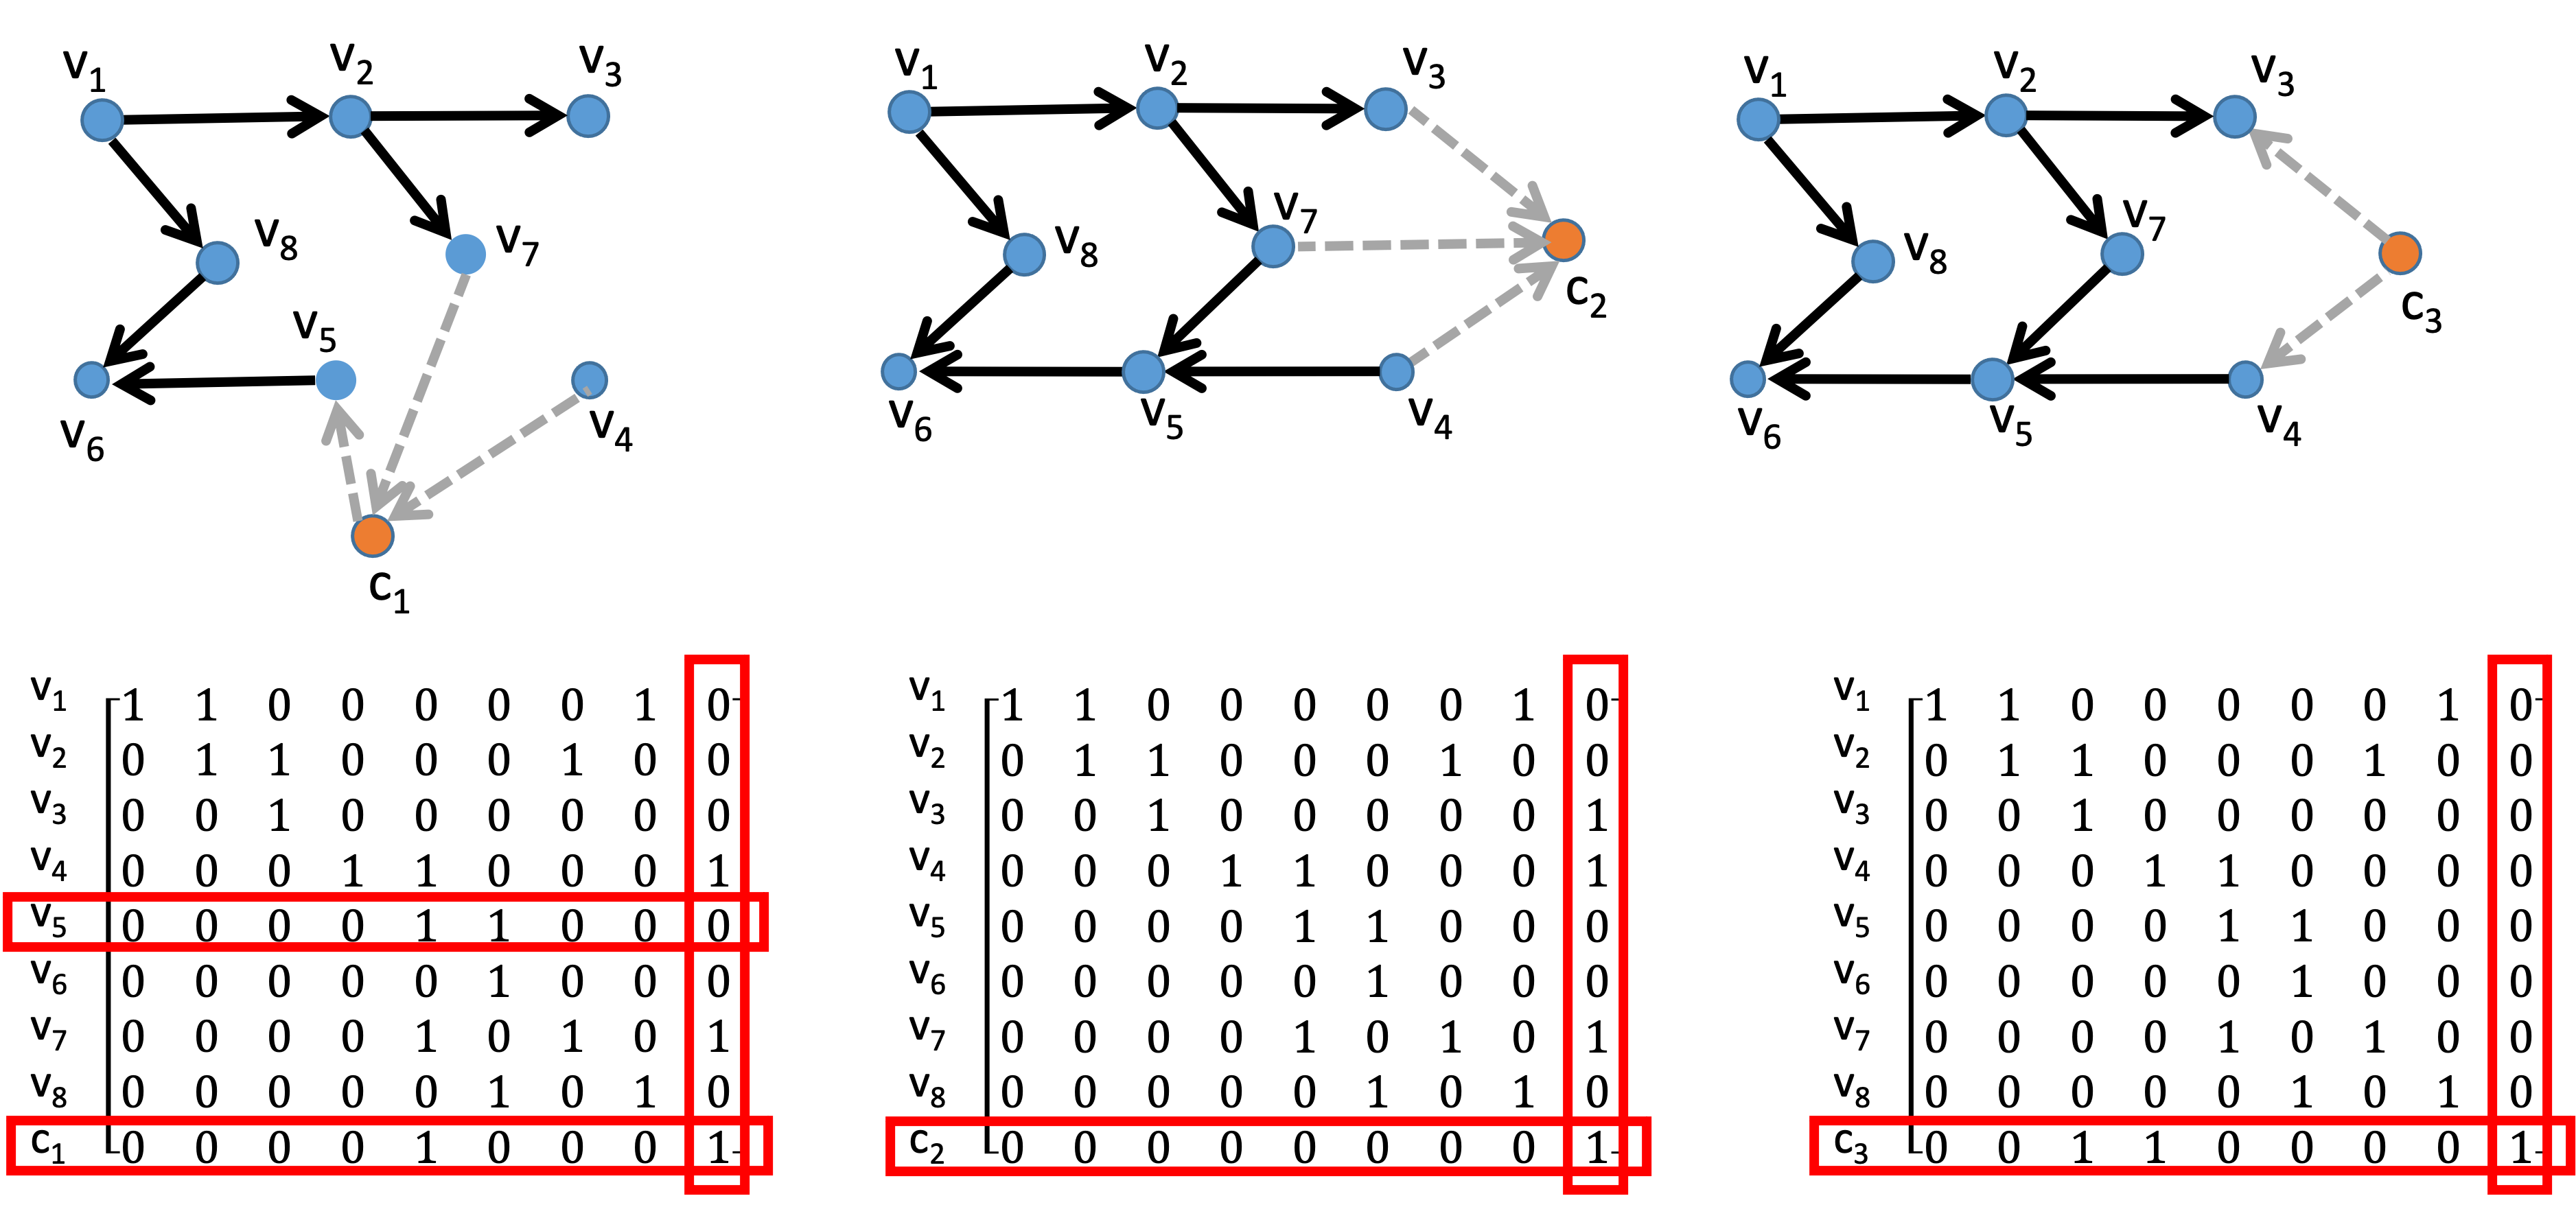
\includegraphics[width=1\linewidth]{fig/event_graph.png}
    \caption{三种时空事件的时空图虚拟节点表示方法}
    \label{fig:event_graph}
\end{figure}

其次,我们需要将时空事件在时空图的结构中进行表示和融合,以便于后续对其进行表征学习。本课题的思路是将时空事件表示为时空图上的虚拟节点,将事件与原有图节点的直接关系表示为虚拟边,将时空事件表示为对原有时空图的一种``编辑''。图~\ref{fig:event_graph}给出了三个具体的示例。其中图~\ref{fig:event_graph}(左)的例子表示在路段$r_5$上发生交通事故,即时空图表示中的节点$v_5$。该事件可以被表示为一个新的虚拟节点$c_1$。由于该事件发生在节点$v_5$上,故而$v_5$原有的入边将被修改为经过$c_1$后再指向$v_5$,而其出边不受影响。原有边$v_7\rightarrow v_5$和$v_4\rightarrow v_5$将被移除。这一操作会修改时空图的邻接矩阵,包括新增一行一列以及修改原有的一列(图~\ref{fig:event_graph}左下)。图~\ref{fig:event_graph}
(中)所示例的是发生在$v_3$,$v_7$和$v_4$附近的大型演唱会(聚集事件)。假设根据事件具体信息,所有的交通流量会经过这三个节点流入事件所在区域。相对应地,事件被表示为图中的一个虚拟节点$c_2$。同时,新建三条虚拟有向边$v_3\rightarrow c_2$,$v_7\rightarrow c_2$,$v_4\rightarrow c_2$来刻画交通流向的变化。类似地,图~\ref{fig:event_graph}(右)所示例的是同一位置演唱会结束之后散场的事件。假设由于交通管制,只有$v_3$和$v_4$可以退场,新的图结构则包括两条从$c_3$发出的有向边,分别指向$v_3$和$v_4$。

通过以上形式化定义和建模,每个时空事件的图结构信息将表示为一个对原时空图进行编辑的操作。该操作将图邻接矩阵的维度从$N$变为$N+1$,同时修改原图中的一些数值。用户给出的时空事件条件可以依据该模型进行信息提取,表示为一个新的邻接矩阵。%形式化地,每个事件$c$的图结构信息可表示为$\Delta_c(\mathcal{G}_T)$,事件发生后新的时空图结构则为$ \mathcal{G}_T\bigcup\Delta_c(\mathcal{G}_T)$。当有多个事件同时发生时,整个事件集合$C$对应的新的图结构信息可表示为$\mathcal{G}_C = (\bigcup_{c\in C}\Delta_c(\mathcal{G}_T))\bigcup\mathcal{G}_T$。
以上时空事件的图结构建模可以应用在除交通推演以外的其他应用场景下,例如河水流速流量推演、地区间人口流动推演等。本课题将在研究中具体实现并验证以上形式化定义思路在其他应用场景下的结果。%我们将在下一章节介绍如何对事件和图结构进行联合表征学习的技术路线。

\textbf{(2) 时空事件的几何-图联合表征学习。}
时空事件的表征学习是为了提取事件的隐含信息,刻画其对时空图节点上属性的影响。事件的影响力不仅取决于事件的本身信息,也取决于事件发生周围的时空图节点的空间属性,例如路段、河流段的位置和形状等。在2.2.1种给出的问题形式化定义中,我们将事件$c$与时空子图$\mathcal{G}_g$共同作为生成条件。因此,表征学习阶段,我们将对事件与时空子图数据进行\textbf{联合表征学习},直接提取事件对每个图节点的影响力程度作为生成条件的嵌入向量$z_g$。

时空事件的表征学习包括两个层次,第一个层次是空间几何表征学习,第二个层次是图拓扑表征学习。这两个层次分别提取时空事件在欧氏几何空间和图拓扑空间上的影响力特征。这里我们需要对欧氏几何空间影响力进行提取是因为在一些应用场景中,事件的影响力并非单纯在图拓扑结构上传播,例如降水量对周围河流的影响同样可以沿地面传播。依据图~\ref{fig:embed}中给出的框架,我们需要学习一个几何信息提取编码器和一个图信息提取编码器,分别提取出不同的影响力信息,再将其结合给出事件和子图之间的联合嵌入向量。

\textbf{首先,我们描述几何信息编码器的设计思路}。本课题对事件的几何影响力进行一种结构化的表征提取。具体地,事件对周围图节点的几何空间影响力可以用任意二维空间的核函数来刻画。不失一般性地,我们用一个高斯核函数来举例。我们定义以$s_0$为中心点,以$\sigma$为带宽(bandwidth)的高斯核函数为:
\begin{equation}
    G_{s_0}(s) = \frac{1}{2\pi\sigma^2}e^{-\frac{(d(s,s_0))^2}{2\sigma^2}}
\end{equation}
这里,我们假设该核函数在各个方向的带宽相同,即无方向性。$\sigma$是一个可以定义的参数,$d(s,s_0)$表示$G$影响范围内的某个点$s$距离核函数中心点$s_0 = (lng_0, lat_0)$的欧式距离。我们假设事件在欧氏空间的影响力可以用一组不超过$m$个具有不同$\sigma$和$s_0$参数的高斯核函数来拟合。为了保证这些高斯核函数的合理性,我们根据事件形状坐标的取值范围对$s_0$进行归一化处理,保证所有的$s_0$都在事件范围内,或事件形状的边界框(bounding box)内。这里,核函数的形式可以进行其他选择。本课题将对其效果进行评估。
\begin{figure}
    \centering
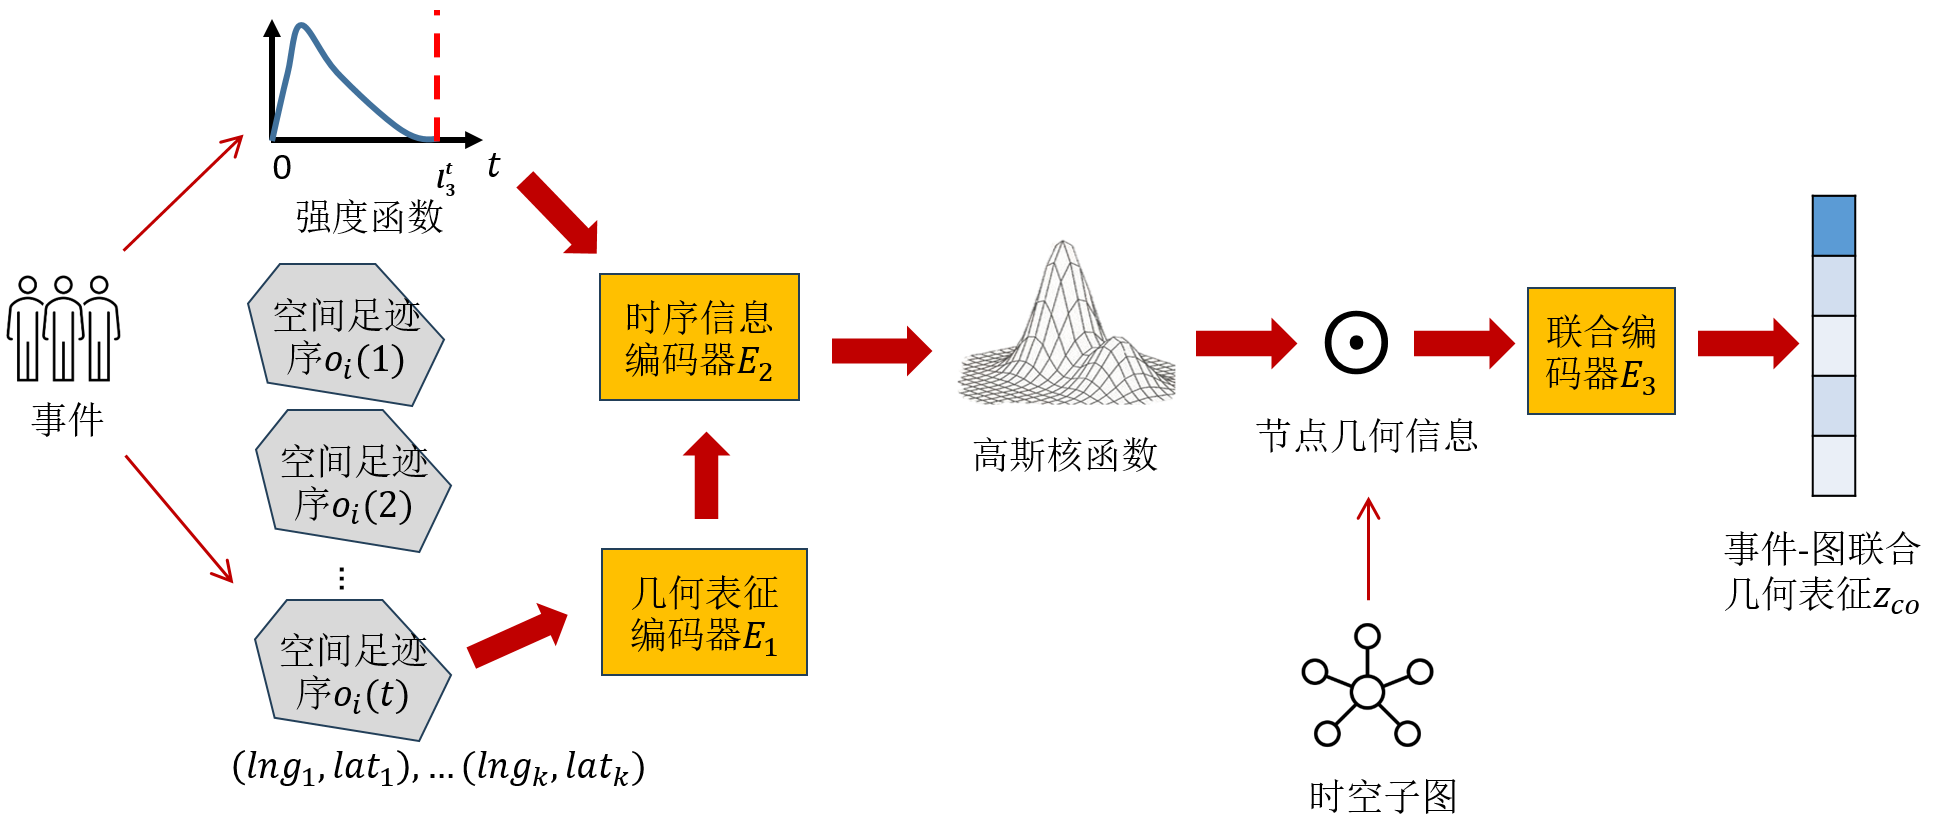
\includegraphics[width=0.99\linewidth]{fig/geo-embed.png}
    \caption{事件-图几何表征提取过程示例}
    \label{fig:geom_encode}
\end{figure}
我们可以将事件几何坐标序列和事件强度函数作为输入送入几何表征编码器$E_1$和时序信息编码器$E_2$,得到一个$3\times m$向量作为事件的几何表征向量。事件几何形状的坐标点序列表征学习需要满足起始点不变性,即从不同顶点开始的输入序列不影响结果。一种相关研究中提出的方法是采用一维卷积神经网络加上循环填充(circular padding)来作为几何属性的编码器。最后,将编码的几何形状时间序列和时间强度学列送入LSTM或Transformer等序列编码器,生成事件的表征向量,即高斯分布参数。图~\ref{fig:geom_encode}给出了一种实现策略的例子。

事件的影响力也取决于事件发生周围的时空图节点的空间属性,例如路段、河流段的位置和形状等。具体地,我们提取子图$\mathcal{G}_g$内所有节点的空间几何信息$v.o$(由$k$组二维坐标序列表示),计算每个坐标点受到$m$个核函数影响力的总和,再计算每个节点受到的平均影响力。%由于不同地区的影响力衰减程度不同,我们为每一个坐标点定义一个参数$w$。
具体的影响力评估函数如下:
\begin{equation}
    F(c, v) = \frac{1}{k}\Sigma^k_{i=1}\Sigma_{j=1}^m G_j(lng_i, lat_i)
\end{equation}
最后,每个节点上的影响力值$F(c, v)$经过一个联合编码器$E_3$转换为事件-图几何表征向量$z_{co}$,$E_3$可由全连接神经网络实现。

下面,我们介绍第二个编码器,即\textbf{图表征提取编码器的设计思路}。这一过程的目的是提取事件沿图拓扑结构对节点产生的影响力。%不同于常见的图节点嵌入方法,这里我们只关心事件对,所以节点间的影响关系是从事件节点到普通节点。
具体地,如图~\ref{fig:embed-bfs}所示,假设该影响力可以用以$c$节点为出发点的定向游走函数来表示。游走函数的设计有多种选择,例如基于深度优先或广度优先的随机游走等。这里我们可以采用广度优先游走结构,即定义一个以$c$为根节点,深度为$l_c$的广度优先搜索树,并定义每一步广度优先游走的影响力函数为$\Gamma(c,i)\in\mathbb{R}^{d_X}$,$i$为游走的步数。我们针对$c$节点的入边和出边两个方向分别定义不同的广度优先影响力函数,即正向的$\Gamma^+$和反向的$\Gamma^-$函数,这两个函数可以看作是学习到的图卷积核。$\Gamma(c,i)$为一个$d_X$维的参数向量。由于事件影响力随着举例衰减,我们定义每个参数为上一步影响力的衰减系数。$\Gamma(c,i,j) \in (0,1]$, $\Gamma(c,0, j)=1$。

为了获得$\Gamma$函数的参数,我们利用拓扑表征编码器$E_4$对事件编辑过的子图$G_c$进行图嵌入,再将结果送入拓扑时序编码器$E_5$,与强度函数经过联合编码后输出。其中$E_4$可以用图卷积神经网络实现,而$E_5$可以采用和$E_2$相似结构。经过联合编码得到两个$\Gamma$函数的所有参数。获得这些参数之后,我们将两个函数作为图卷积核,对输入的子图数据$\mathcal{G}_g$进行图卷积操作,获得每个图节点上对应的影响力嵌入,最后通过联合编码器$E_6$得到事件-图联合拓扑表征向量$z_{cg}$。最后,将$z_{co}$与$z_{cg}$拼接即可获得事件-图联合表征向量$z_c$。
\begin{equation}
z_{cg} = E_6((\prod_{j=1}^{i}\Gamma(c,j)) \odot \mathcal{G}_g.\mathbf{X})
\end{equation}
%每个节点上的属性值根据距离$c$的步数与影响力函数对应值相乘,得到对事件每个图节点的``影响力''评估。我们通过训练图表征提取编码器来获得$\Gamma^+$和$\Gamma^-$的参数。
\begin{figure}
    \centering
    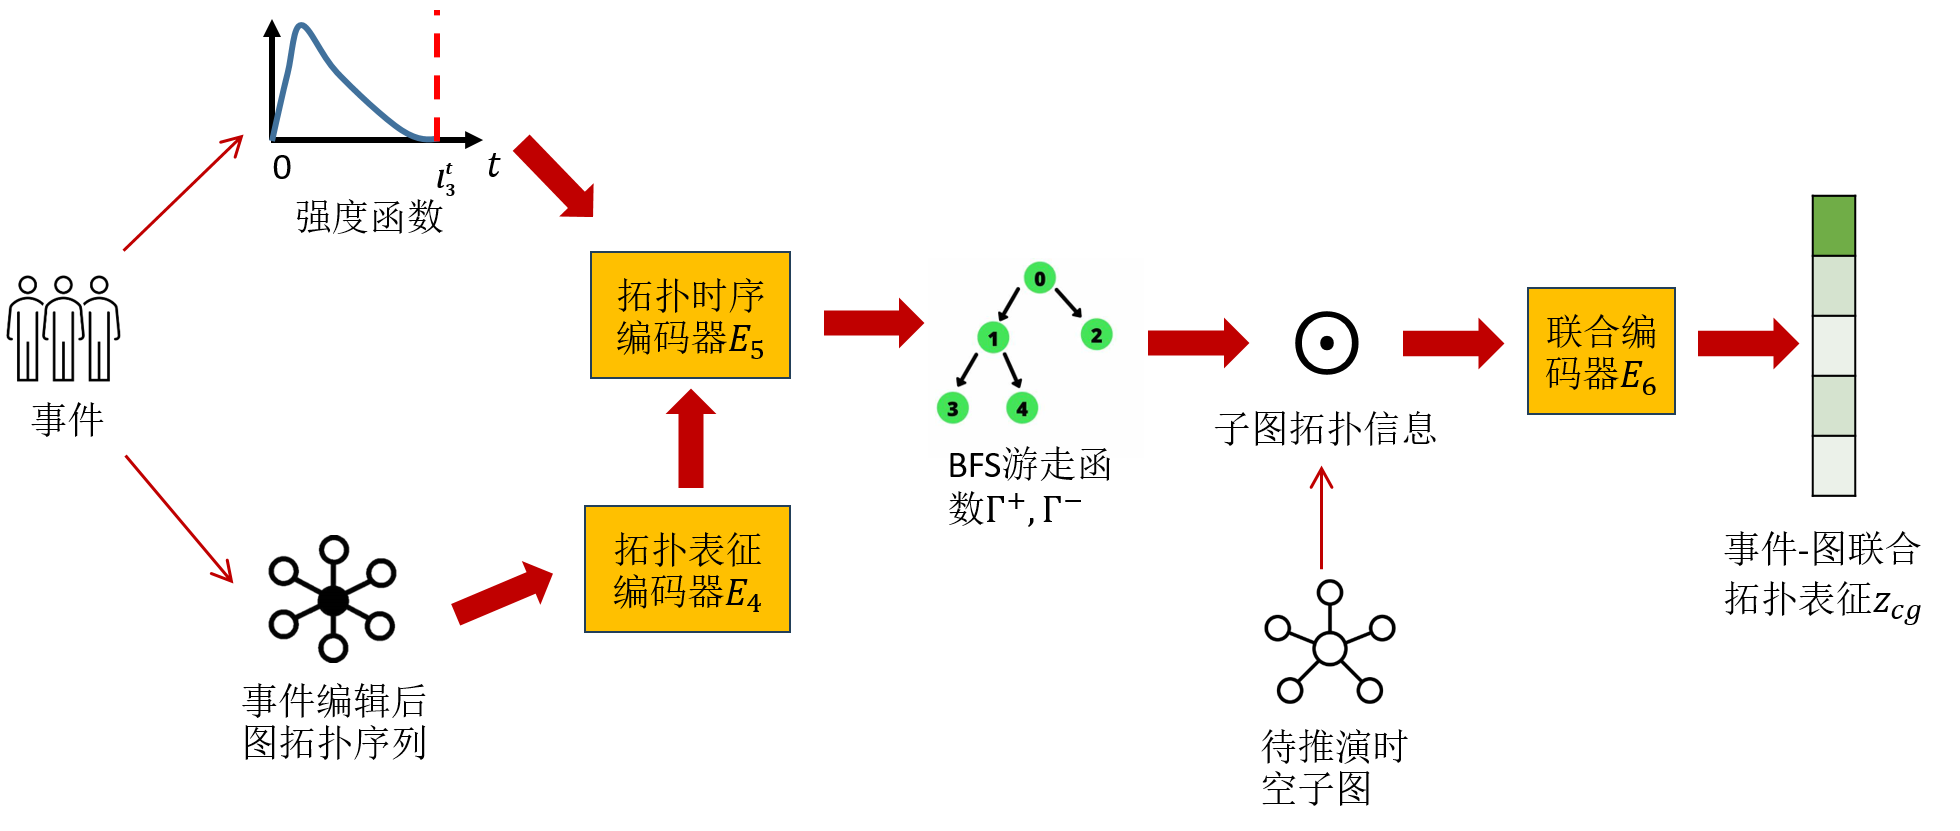
\includegraphics[width=1\linewidth]{fig/topo-embed.png}
    \caption{事件-图联合拓扑表征提取流程示例}
    \label{fig:embed-bfs}
\end{figure}
最后,我们介绍如何对以上\textbf{两组编码器模块进行联合训练}。这里我们可以通过一个编码器-解码器结构对表征学习网络进行单独的与训练,获得其参数;也可以将上述网络接入子图生成网络,进行端到端的训练。一个简答的与训练思路是利用嵌入向量$z_g = z_{co}||z_{cg}$通过一个参数化解码器$D$直接对目标属性$\mathcal{X}\in \mathbf{X}$在$\mathcal{G}_g$上进行预测,通过均方误差(MSE)等损失函数对模型参数机型训练:
%对事件信息和事件发生前的时空图$\mathcal{G}^*_T$进行联合编码,然后再对其进行解码来对事件发生后的时空图数据进行拟合。具体地,针对一个输入事件$c$和一个子图$\mathcal{G}^*_T$,我们将几何信息编码器的输出$z^t_{co}$和图信息编码器输出$z^t_{cg}$拼接作为总编码信息$z^t_c$。再将$\mathcal{G}^*_T$上的事件前数据$X_T$与$z^t_c$送入解码器进行联合解码,应用同样的高斯核函数和广度优先树卷积核来生成出事件后的新数据$\tilde{X}$。最后通过真实的事件后数据$X$与$\tilde{X}$来定义损失函数。
%图~\ref{fig:event-overall}给出了这一过程的示例。其
\begin{equation}
    \mathcal{L} = \Sum\frac{1}{|\mathcal{G}_g|\times L}||\mathcal{X} - \tilde{\mathcal{X}}||_2
\end{equation}
%上述思路仅提供了对事件表征进行学习的一种预训练方案。我们也可以将上述表征学习的编码器网络和后续的图生成模型连接,进行联合训练。具体的几何与图卷积核函数的选择,以及深度学习网络结构的设计需要本项目进行深入研究。
这里我们没有对数据分布进行学习,也没有对自相关性、异质性等问题进行解决,故而不能直接得到本问题的输出。但是可以作为一种预训练方法来获取生成条件的嵌入向量。本课题将对以上过程种的具体算法步骤、编码器结构设计以及训练方法等方面进行具体研究。
% \begin{figure}
%     \centering
%     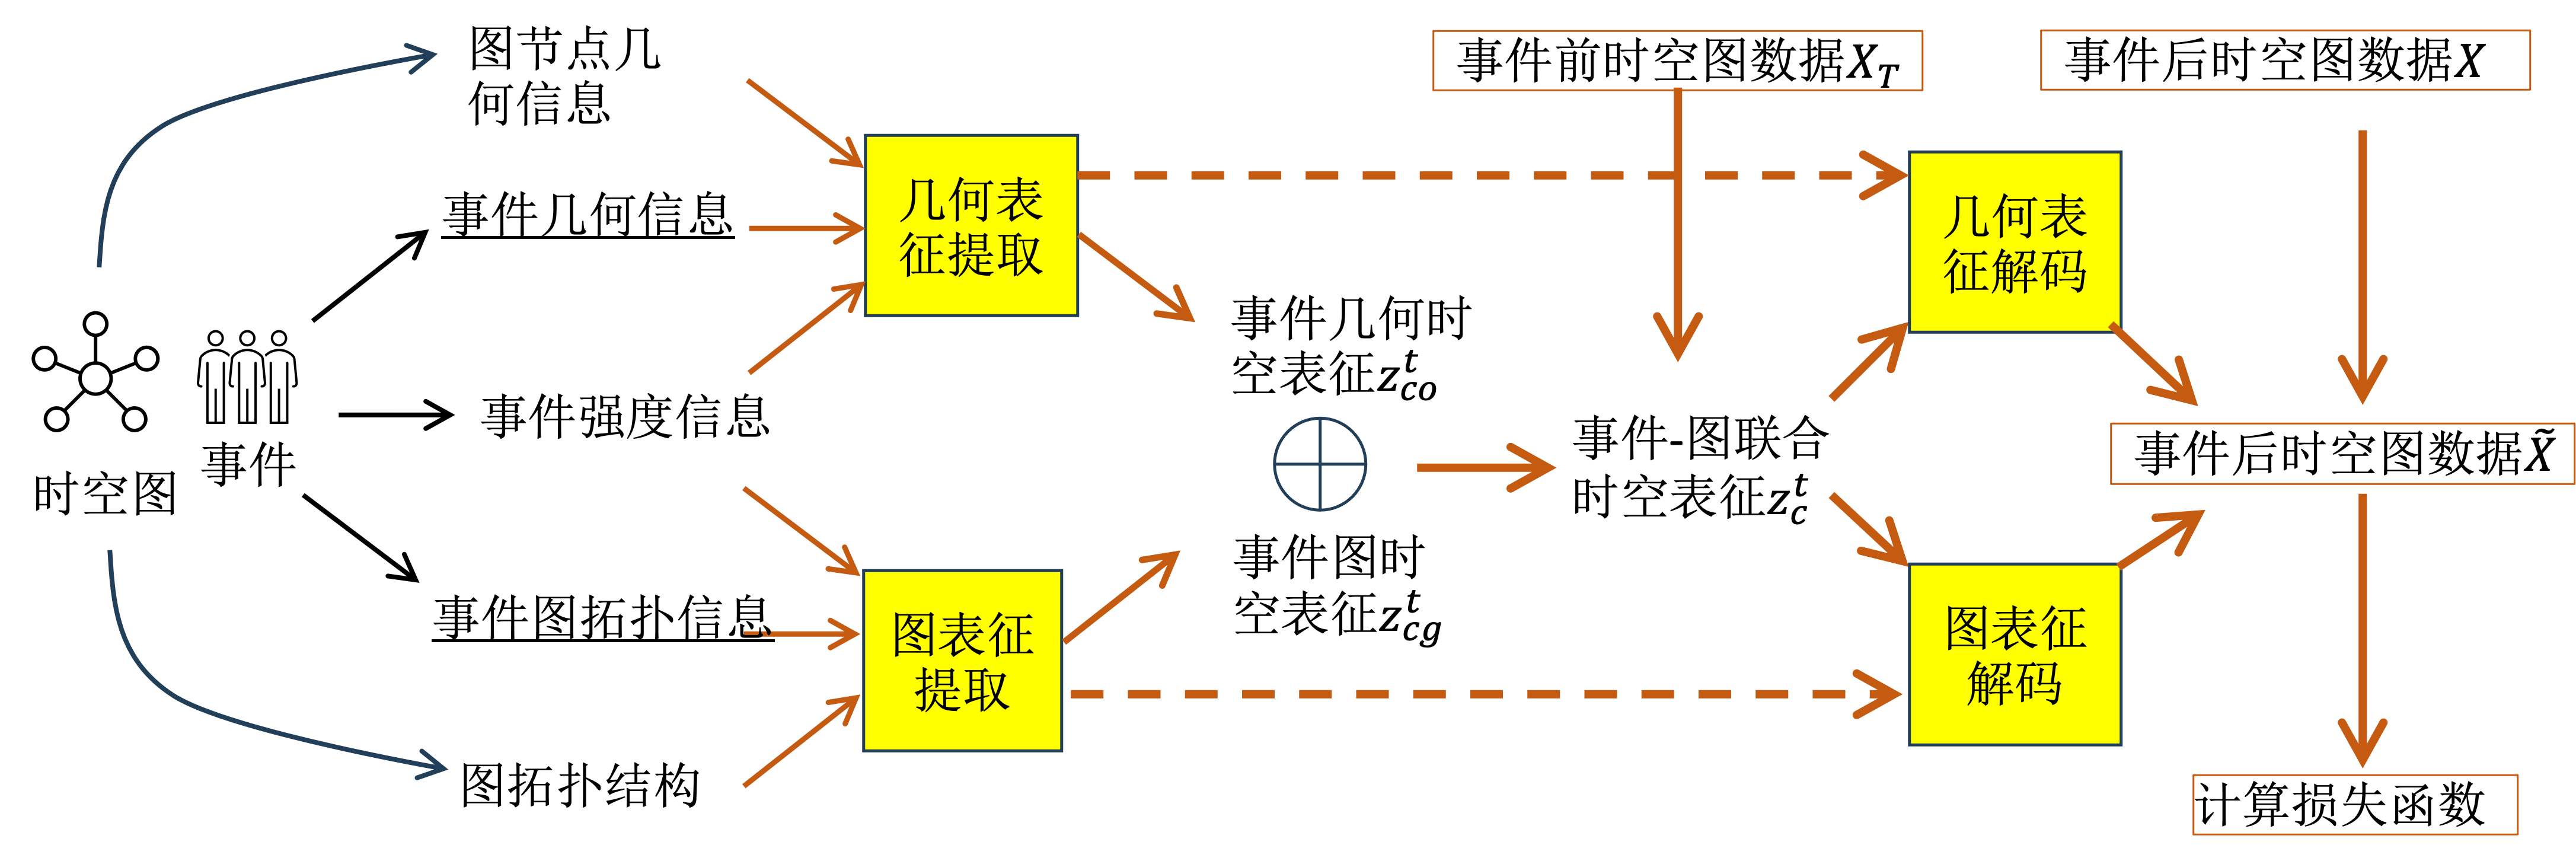
\includegraphics[width=0.99\linewidth]{fig/event_encode_overall.png}
%     \caption{时空事件的几何-图联合表征学习框架}
%     \label{fig:event-overall}
% \end{figure}

\subsubsection{3.1.2 基于自相关隐变量空间的时空子图生成}
\textbf{(1)相关性子图划分:}如前文所述,为了实现自相关的子图生成,本课题先对输入的时空图进行子图划分。子图划分的目的是构建基本的数据生成单元,目标是将具有数据相关性的节点划入同一子图,从而提高模型训练的效率。由于子图结构没有``正确''样本来进行学习,所以我们无法通过训练一个图嵌入模型来进行聚类或者划分。这里,我们设计一种可行的启发式搜索方法进行划分。具体地,每次随机选择一个开始节点,通过广度优先搜索的方法评估每个候选节点,并选取对目前子图``贡献''最大的节点,重复这一步骤直到达到子图最大节点数。

这一步骤的核心是定义一个函数来评估每个节点对当前子图的贡献度。这里我们需要考虑两个因素:(1)提图中节点数据的相关性,(2)减少图结构的重叠性。根据这两个原则,我们可以定义一个类似于如下的混合评价函数:
\begin{equation}
    \Lambda(\mathcal{G}_i, v) = \lambda_1 \min  \{Corr(X_v, X_{u,u\in\mathcal{G}_i})\}-\lambda_2 I(v\in \mathcal{G}_j,j\ne i)
\end{equation}
其中$\matchal{G}_i$为一个目前待扩张的子图,$Corr$为历史数据的相关性,例如Pearson相关性系数等,可由每个节点的历史数据时间序列计算得出。第一项计算每个新节点$v$与已有节点之间最小的数据相关性。这里也可以用加权平均的方法,计算$v$与$\mathcal{G}_i$中所有已有节点的相关系数并根据二者的图拓扑距离进行加权平均,距离越远则权重越小。
第二项中,$I()$为计数函数,表示节点$v$已经被包含在其他子图中的次数。通过$\lambda_1$和$\lambda_2$可以对两部分权重进行调整。为了减少起始节点选择对结果造成的影响,我们可以选取多个随机的起始节点,并轮流进行节点添加。由于节点间的相关性系数可以根据历史数据提前计算,故而以上子图划分可以通过预存储部分结果的方法提高计算效率。本课题将深入研究划分算法的具体步骤和提高划分计算效率的技术。

\textbf{(2)基于自相关隐变量的子图生成学习模型}。本课题的核心是研究如何建立一个基于高斯马尔科夫随机场的自相关性子图生成模型。首先我们介绍高斯马尔科夫随机场的基本模型和概念。给定一个无向图结构$G(V, E)$,$\mathbf{X}$是节点$V$上的一个随机变量,即$\mathbf{x} = ({x}_v)_{v\in V}$。变量$\mathbf{X}$在满足马尔科夫属性时,可称为一个马尔科夫随机场。马尔科夫属性指每个节点上变量${x}_v$的分布只与其相邻节点上的变量${x}_u$相关,而与其他节点上的变量独立。形式化地,$p({x}_v|{x}_{u, u\ne v}) = p({x}_v|{x}_{u, u\in N(v)})$,$N(v)$为节点$v$在图$G$中的直接邻居节点集合。
%当每个节点存在隐变量$\mathbf{Z}$,且每个节点的数据分布概率仅受到本节点上隐变量$\mathbf{Z}$的影响时,我们可以定义该马尔科夫随机场为一个隐变量马尔科夫随机场。
当每个节点的变量$\mathbf{x}$符合高斯分布的时候,该随机场即定义为高斯马尔科夫随机场(GMRF),即$\mathbf{x}\sim\mathcal{N}(\boldsymbol{\mu}, {Q}^{-1})$,其中${Q}^{-1}=\Sigma$为不同节点上$x$的协方差矩阵,而${Q}$为相应的精度矩阵。基于前述马尔科夫假设,当节点$u$和$v$不为邻居时,${Q}^{-1}_{uv} = 0$。而所有变量$X$的联合概率密度函数为:
\begin{equation}
    p(\mathbf{x}) = \frac{1}{(2\pi)^{n/2} |Q|^{1/2}} \exp\left(-\frac{1}{2} (\mathbf{x} - \boldsymbol{\mu})^T Q (\mathbf{x} - \boldsymbol{\mu}) \right)
    \label{eq:7}
\end{equation}
其中$|.|$为计算行列式操作。

在本问题中,我们将划分好的子图表示为超节点,将子图间的关系表示为一个无向超图$\mathcal{G}^s$。同时,我们可以定义$\mathcal{G}^s$上的邻接矩阵。例如,一种简单的方法是当两个$\mathcal{G}$上的有向子图有交集时,则这两个子图对应的超节点成为超图$\mathcal{G}^s$中的邻居节点。假设$z_g$为子图$\mathcal{G}_g$上数据分布对应的隐变量,我们可以将所有子图数据对应的隐变量$z$表示为一个高斯马尔科夫随机场(GMRF)。

这里我们合理地假设两个有向子图之间的关联性由他们共同相交的子图传递,而这两个子图之间的数据分布相互独立。这样我们可以利用高斯马尔科夫随机场的模型来对超图$\mathcal{G}^s$建模。具体地,我们将子图隐变量的联合先验分布选择为一个零均值的高斯马尔可夫随机场。在给定的生成条件嵌入$z_{gc}$下(3.1.1中已介绍),所有子图$\mathcal{G}_g\subseteq\mathcal{G}$的对应隐变量$z_g$的联合分布可表述为:
\begin{equation}
{z_{g}}|{z_{cg}}\sim\mathcal{N}(\mathbf{0}, {Q}^{-1})
\end{equation}

其中,当子图$i$和$j$对应的超节点不为邻居时(即子图$i$和$j$不重叠时),${Q}^{-1}(i,j) = 0$。$Q_{ii} = \frac{1}{\sigma(z_i)}$。需要说明的是,同经典的VAE模型一样,我们这里假设$z$的所有维度相互独立,且都服从同一个GMRF分布,故而可以用同一组参数表示。

%求得的高斯马尔科夫随机场进行采样来获得隐变量$z_{g}$,(3)如何对$z_{g}$解码进而生成相应的图数据。
%得到GMRF的参数化刻画之后,我们可以利用Mean-Field近似,Gibbs采样等多种方法对GMRF进行采样

%求解整个$\Tilde{Q}$在计算上具有很大挑战性。在本课题中,局部子图生成不需要获得整个$\Tilde{Q}$值。

\textbf{本课题拟设计一个基于变分自编码器(VAE)思路的联合训练架构实现端到端的自相关子图生成}。VAE架构的优点是可以自然地采用贝叶斯学习的方式定义变量间的生成关系,获得统计上合理的数据分布,同时相较于GAN模型更易于训练,而比Diffusion模型生成时的计算效率更高。经典的图变分自编码器(GraphVAE)包括一个参数化编码器$q_\phi(z|x)$,来近似$z$的后验概率分布,将输入的图数据映射到$z$的分布空间上。同时训练参数化的解码器$p_\theta(x|z)$,即数据$x$的似然值。$p(z)$为隐变量的先验概率,通常都假设为一个独立随机的标准高斯分布。解码器则对采样的$z$进行解码生成具体的图数据。当进行条件生成时,条件变量$c$可以被加入到编码器中作为输入。由于本问题不涉及邻接矩阵的生成或边属性的生成,所以解码器的重建损失函数只有一项,即节点属性的后验概率。加入生成条件$c$后,VAE模型的训练都可以通过对最大化经验最小下界ELBO(Evidence Lower Bound)来进行:
\begin{equation}
    \mathcal{L} = \mathbb{E}_{\phi(z|x,c)}[\log p_\theta(x|z,c)]-KL[q_\phi(z|x,c)||p(z|c)]
\end{equation}
其中KL散度函数计算拟合的后验概率$q_\phi(z|x,c)$与先验概率$p(z|c)$的相似度。在常见的基于VAE的模型中,$p(z|c)$经常被设定为服从一个标准高斯的先验分布。

\underline{在自相关性隐变量假设下},我们需要将先验概率$p(z|c)$替换为上述定义的高斯马尔科夫随机场(GMRF)。当均值$\mu=\mathbf{0}$时,公式~\ref{eq:7}可简化为:
\begin{equation}
    p(z|c) = \frac{1}{(2\pi)^{n/2} |Q|^{1/2}} \exp\left(-\frac{1}{2} \mathbf{z}^T Q \mathbf{z} \right)
        \label{eq:pz}
\end{equation}
$Q$为需要指定的参数。除了修改先验分布$p(z|c)$,编码器$q_\Phi(z|x,c)$也需要根据数据拟合出后验概率的参数,即向量$\mathbb{\mu}$和$Q$矩阵。而$p_\theta$则需要根据拟合出的GMRF进行采样来计算似然值。另外,KL散度的计算也相应改变。我们需要计算两个GMRF,$p$和$q$之间的KL散度,其中$p$的均值为$\mathbf{0}$。具体计算方法如下:
\begin{equation}
    {KL}(q || p) = \frac{1}{2} \left( \text{tr}(Q_p Q_q^{-1}) - \log \frac{|Q_p|}{|Q_q|} - n + \boldsymbol{\mu}_q^T Q_q \boldsymbol{\mu}_q \right)
    \label{eq:kl}
\end{equation}
其中tr()为方阵的迹,即对角线元素之和;$n$为变量$Z$的维度,即GMRF节点数;|.|为求行列式运算。$\boldsymbol{\mu}_q$和$Q_q$分别为后验概率分布(即编码器$q_{\phi}$)给出的估计均值向量和精度矩阵。$Q_p$为模型指定的先验GMRF的精度矩阵,为常数。最终,我们给出新的模型GMRF-cVAE的损失函数为:
\begin{equation}
    \mathcal{L} = \mathbb{E}_{\phi(z_g|\mathcal{G}_g,z_{cg})}[\log p_\theta(\mathcal{G}_g|z_g,z_{cg})]-KL[q_\phi(z_g|\mathcal{G}_g,z_{cg})||p(z_g|z_{cg})]
    \label{eq:gmrf_loss}
\end{equation}
其中$\mathcal{G}_g$为待生成的子图数据,$z_g$和$z_{cg}$分别为子图$\mathcal{G}_g$的隐变量和事件$c$的表征向量。
基于一般VAE的通行的假设,我们可以进一步对参数进行简化。假设对所有子图,$z_g|z_{cg}$的分布都具有相同的均值$\mu$和标准差$\sigma$,则编码器需要拟合的参数变为一个标量$\mu$,一个标量$\sigma$($Q_{ii}$倒数值),以及所有用来描述超节点间相关性的变量$Q_{ij}$值。相比于传统GraphVAE或一般VAE,只有最后一项是我们需要拟合的额外分布参数。

对模型训练时,我们训练编码器$q_\phi$根据输入的生成条件和输入的事件后观测数据来拟合出${\mu}$,$\sigma$两个全局参数,和所有$Q_{ij}$值。通过这些参数,我们对GMRF进行采样,获得一个$\mathbf{z_g|z_{cg}}$的样本。再通过样本的解码用$p_\theta$生成图$\mathcal{G}_g$的数据。

因此,\textbf{本问题的核心}转变为(1)如何设计先验概率$p(z_g|z_{cg})$,即如何设计$Q_p$矩阵来反映子图的时空自相关约束,(2)如何设计新的VAE模型结构对子图数据进行编码,使其能够拟合上述三组参数。(3)如何对拟合出的GRMF进行高效采样来降低计算开销。

\underline{对于$Q$矩阵的设计}:精度矩阵元素$Q_{ij}$的取值取决于超节点(即子图)间的空间依赖关系。一种可行的方案是对超图
$\mathcal{G}^s$求取拉普拉斯矩阵并将其作为$Q$矩阵。这种方法是直接根据图的邻接关系来定义。%图~\ref{}给出了一种$Q$矩阵取值的例子。
\textbf{本课题将针对这些选择进行深入研究并设计合理的$Q$矩阵}。
\begin{figure}
    \centering
    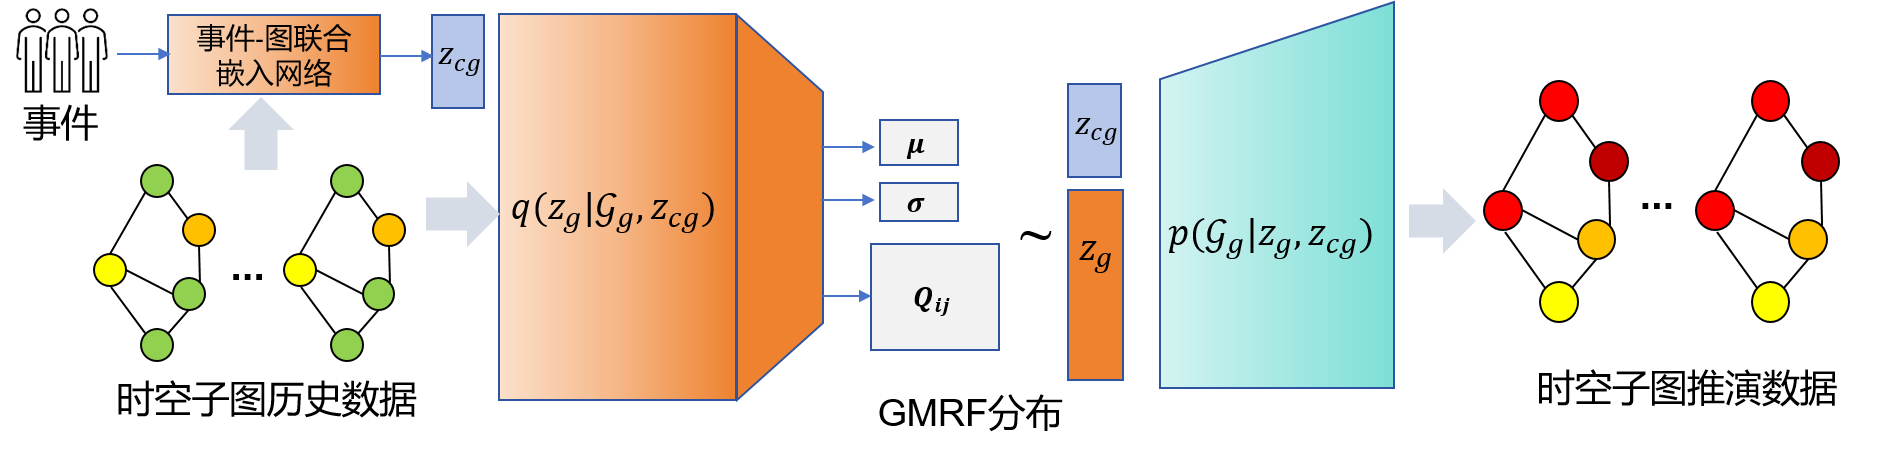
\includegraphics[width=1\linewidth]{fig/gmrf-vae.png}
    \caption{本研究中提出的基于GMRF的子图生成模型结构示意图}
    \label{fig:gmrf_vae}
\end{figure}

\underline{对于模型设计},图~\ref{fig:gmrf_vae}给出了拟研究的基于GMRF的子图生成模型架构概念图。我们首先设计一个双层时空图卷积网络编码器来实现对每个子图及其邻接子图嵌入学习。对于$\mu$和$\sigma$两个参数,我们使用与传统GraphVAE相同的策略,应用时空图卷积网络(ST-GCN、T-GCN)等模块对所有子图样本进行全局训练,拟合出这两个参数。对于$Q_{ij}$参数,我们提取每个子图$G_g$及其所有邻居子图$\mathcal{N}(G_g)$,通过对这个子图群应用时空图卷积操作对每个矩阵行$Q_i$进行预测。由于$Q$是角对称矩阵,我们只需对一半的参数进行拟合即可。因为$Q$是稀疏矩阵,每个子图的邻居子图数量有限,故参数规模在可控范围内。\textbf{本课题将对模型结构的具体设计进行深入研究}。

%由于子图构成的超图是无向图,$Q$矩阵是对角线对称矩阵,所以编码器只需要对每行数据进行近似。我们使用
\underline{对于GMRF采样方法},常用的采样方法是对稀疏的正定矩阵$Q$进行Cholesky分解得到$Q=LL^T$,$L$是下三角矩阵。我们先生成$N$个标准高斯分布样本$\mathbf{Z}\sim\mathcal{N}(0, \mathbf{I})$,$N$为超图中总节点数。然后利用$L\times Z$将$Z$变换为符合自相关性的采样值,从而获得$z_g$及其他子图的隐变量采样值。为了保证分解的可行性,我们需要保证$Q$的正定性。同时,为保证求解过程中变量的可微性,我们需要对Cholesky分解的实现步骤进行研究,保证其能够通过反向传播训练。\textbf{本课题将对以上模型设计中的具体问题进行研究,并研究以上方法的实际效率以及可能的改进提高策略}。

\textbf{(3)模型训练样本构建和采样策略。}由于本问题中,训练样本需要和事件匹配,故我们需要为上述的模型设计一个训练数据集构建的方法。首先,对每一个子图,我们搜索其周边距离$d$以内的每一个事件,根据事件发生的时间,提取子图上相应数据,和子图结合生成条件联合嵌入$z_{cg}$。同时,提取事件发生后图上数据作为目标变量的样本。对于周边没有事件发生的的子图,则采取两种办法:1)增大搜索范围,找到距离该子图最近的事件,并构建训练集,2)直接使用无事件的历史数据作为生成条件获取嵌入表征,即只用该子图上的历史数据作为条件获得$z_{cg}$。在模型训练时,我们需要对训练样本进行采样并送入模型。在对\underline{全局变量$\mu$和$\sigma$的训练}中,我们只需要对部分子图进行采样即可。采样策略应注重地理分布的均衡性。本课题拟设计一个重要性采样(importance sampling)方法,对每个子图给出一个采样概率。每轮采样过后,被选中的子图周边子图的采样概率将被下调,而其他地区的采样概率上升。同时,如果一个子图附近没有事件可以匹配,则该地区样本对全局模型的贡献较小,故而可以对其采样概率下调。我们可以基于该子图和其最近事件的距离来设计采样概率的动态调整策略。\textbf{本课题将对这一采样算法进行具体设计和研究}。

在对\underline{每个子图的变量$Q_{ij}$的训练中},我们需要子图和其邻居配对的样本来训练对每个$Q_{ij}$值的拟合。故而,我们需要对每个子图和其邻居进行采样。我们采取类似的策略,即如果一个子图的某个邻居子图已被采样,则下调它在下一轮采样中被选中的概率,保证每个邻居子图都提供足够的样本来进行训练。同时,\textbf{本课题还将研究样本复用方法},即基于已经在全局采样中被选中的样本,通过样本缓存等方式避免反复采样,以提高模型的训练效率。

%最后,我们通过设计解码器$p$来将采样到的隐变量映射回图数据空间。这里我们采用和GraphVAE类似的结构,将事件条件的嵌入表征向量$z_c$和子图采样隐变量$z_g$作为输入送进图解码器,得到对事件条件下图数据预测值$\Tilde{X_g}$。

%%如何对没有样本地区进行估计和采样??
%以上模型架构的训练中,涉及到前述的对GMRF进行采样,以及对KL散度的计算开销较大。本课题拟对如何高效地进行这些计算进行深入研究。

%在对模型进行训练时,由于整个时空图规模较大,所以编码器不能对整个$Q$进行拟合。由于$Q$是稀疏矩阵,我们可以将它分割为独立单元,并单独训练。

% 其次,我们将上述编码器和解码器作为预训练模型,将DGMRF网络接入,对整个模型进行再训练来获得DGMRF的参数。图~\ref{}给出了这一设计的示意图。训练时,我们给编码器提供的样本包括每个子图及其邻接子图,即超图上的邻接节点。我们通过编码器获得每个子图的隐变量$z_g$。然后,对生成超子图上的自相关隐变量分布$z_{sg}$,并将超子图结构输入深度高斯马尔科夫随机场神经网络,将其变换为标准独立高斯分布。由于$Q$矩阵的稀疏性,我们通过局部采样的方法,获得矩阵$D$和$A$的局部参数,并对神经网络进行局部参数更新,进而对$Q$矩阵的每个局部进行估计。

% 在进行数据生成的时候,我们使用Gibb采样或Mean-Field近似的方法,对所学习到的局部高斯马尔科夫随机场进行采样,获得每个超子图中节点对应的自相关隐变量采样$z_g$。最终将$z_g$输入训练的解码器中,生成出最终的数据分布。

% 近年来,Siden和Oskarsson等人先后提出了利用深度学习来求解高斯马尔科夫随机场的方法。定义对高斯马尔科夫随机场变量$z$的变换,我们可以将高斯马尔科夫随机场$z$转变为一个符合独立随机标准高斯分布的新的隐变量$\omega$:
% \begin{equation}
% \omega=g(z)=Gz+b,\omega\sim\mathcal{N}(\mathbf{0}, I)
% \end{equation}
% 同时我们有${Q} = G^TG$。将函数$g$的操作分解为一个操作序列$g_0, g_1, g_2, ... g_L$,$g_0\circ g_1\circ g_{2}\circ...\circ g_L(z) = \omega$。这一变换过程可以由一个图神经网络来实现,即深度高斯马尔科夫网络(DGMRF)。其求解过程类似于生成模型中的去噪扩散概率模型的思想。具体地,我们可以定义一个基于信息传递的图神经网络,每一层网络$l$对应操作函数$g_l$。网络中图节点$i$对应的输出为${h}^{(l)}_i$。每个图神经网络层可以定义为:
% \begin{equation}
%     h_i^{(l)} = b_l+\alpha_l d^{\gamma_l}_ih_i^{l-1} +\beta_l d_i^{\gamma_l-1}\Sigma_{j\in n(i)}w_{i,j}h^{(l-1)}_j
% \end{equation}
% \begin{equation}
%         G^{(l)} = \alpha_lD^{\gamma_l}+\beta_lD^{\gamma_l-1}A
% \end{equation}
% 其中$\alpha_l$,$\beta_l$,$b_l$和$\gamma_l$是可训练参数,$n(i)$表示节点$i$的邻居节点,$w_{i,j}$表示节点$i$和$j$之间无向边的权重,$A$为图邻接矩阵,$D$为节点度对角矩阵。通过训练神经网络,获得$Q$矩阵的估计值$\Tilde{Q}$。
%我们除了求解高斯马尔科夫随机场外,还需要学习如何将采样的隐变量映射回图数据上。基于这一需求,我们提一个新的解决思路,即跳过对GMRF进行采样的步骤,直接学习一个从子图数据到

\subsubsection{3.1.3 时空子图的层次化生成学习模型与算法}
在3.1.2中介绍的生成模型中,为了对一个子图上的数据进行生成,我们需要对所有子图的隐变量进行一次采样。这造成了生成方式的不灵活。当进行大尺度的模型生成时,这种方法时较为合理的。但是当我们只需要对一个小的局部子图进行生成时,该策略则代价较高。基于这个观察,我们提出利用层次化生成的策略进行子图生成。具体研究思路如下:

\textbf{(1)层次化的子图结构划分。}对时空图$\mathcal{G}$的层次化划分可以看作是一个多阶段的层次化聚类过程。类似于之前的划分方法,我们可以设计一个迭代过程,在每一层完成子图划分之后,在其形成的超图上再进行下一轮的子图划分,最终完成所有的层级上的划分。这里,层次化子图划分过程与一次划分的主要区别是(1)图属性和事件嵌入表征的重新计算,(2)超图邻接关系的确定。

\textbf{首先},我们需要定义并计算每个超图节点上的属性值。根据2.2.3中的介绍,我们可以对底层属性图上数据进行多轮聚集,例如计算总交通流量、总水流量,或平均车速等参数,获得相应上层子图的属性。这一过程相当于对高分辨率子图进行池化获得低分辨率子图。同时,我们还需要解决时空事件如何对不同层次子图上进行嵌入表达的问题。3.1.1中介绍的事件-子图联合嵌入是在底层时空图上学习到的。如果对每层子图都进行一次嵌入学习,则会造成样本过少,模型复杂的问题。这里我们同样采取池化的思路。第一步,对所有$\mathcal{G}$上同一时间发生的事件,我们使用3.1.1章节中介绍的几何特征编码器和图拓扑编码器对它们逐个进行编码,提取出所有事件对应的高斯核函数与BFS游走核函数。第二步,我们用每一个核函数在原始时空图$\mathcal{G}$上进行卷积操作并获得每个节点受到所有事件的总影响力表征值。之后,我们通过上面对属性聚集时相同的层次化池化的方法,对每一个超节点所覆盖的$\mathcal{G}$上节点的影响力表征进行层次化聚集,最后得到每个超子图上$N_{max}$维的影响力表征向量。进一步通过对其降维(例如使用图~\ref{fig:geom_encode}和图~\ref{fig:embed-bfs}中已训练的联合编码器$E_3$,$E_6$)获得最终每个不同层超子图的条件表征向量$z_{cg}$。

\textbf{其次},我们需要为每一层超图定义邻接关系。在层次化划分的模式下,每一层超图的邻接矩阵可以用不同方式定义。例如,在第一层划分时,我们可以定义具有重叠节点的子图为相邻子图,以此来保证子图的连通性。在更高层级的划分中,由于时空图已经变为无向图,所以我们可以采取其他方式,例如,可以定义“被一条或多条超边连接的两个子图为邻居子图”。进行灵活定义的目的时为了保证每层超图的连通性。这是因为,如果出现了非连通节点,则无法保证所有原图上的子图在同一个层次上进行生成,会对模型训练带来困难。针对不同超图邻接矩阵的定义方式,本课题将对划分的具体算法和评估函数进行详细研究。

\textbf{(2)层次化子图生成模型的设计。} 当层次化子图划分完成后,我们需要建立一个对每层子图进行生成的模型。具体地,我们借鉴层次化变分自编码器NVAE的架构模式。NVAE是一种层次化VAE的设计,用来对图片数据进行层次化生成。相比于本问题,NVAE或类似相关技术没有对空间自相关性隐变量的生成部分,也没有对图数据结构或生成条件进行处理。首先,我们仍然使用公式~\ref{eq:gmrf_loss}中定义的损失函数形式,为每一层的子图训练一个独立的编码器和解码器,其中$l$为超图的层数。
\begin{equation}
\begin{split}
    \mathcal{L}_{l,l\in 1:L} = \mathbb{E}_{{\phi_l}(z^l_g|\mathcal{G}^l_g,z^l_{cg})
    }&[\log p_{\theta_l}(\mathcal{G}^l_g|z^l_g,z^l_{cg},\mathcal{G}^{(l-1)}_g)]\\ &-KL[q_{\phi_l}(z_g|\mathcal{G}^l_g,z^l_{cg},\mathcal{G}^{(l-1)}_g))||p(z^l_g|z^l_{cg}, \mathcal{G}^{(l-1)}_g))]
\end{split}
    \label{eq:hgmrf_loss}
\end{equation}
上式中,$p_{\theta_l}$和$q_{\phi_l}$分别为第$l$层模型的解码器和编码器,$z^l_{cg}$为第$l$层超子图上的生成条件表征向量,$z^l_g$为第$l$层超子图的表征向量。由于我们假设层次间条件独立性,即每个子图的隐变量分布除了服从高斯马尔可夫随机场外,还依赖于上层父超图数据的分布,故每一个条件概率项的输入均添加了$\mathcal{G}^{(l-1)}_g$,即每个超子图的父层子图上的数据。

由于进行了层次化划分,每个超子图大小被限定为$N_{max}$。假设第$l$层有$N(l)$个大小为$N_{max}$的超子图,每个第$l$层超子图$\mathcal{G}^{l}_{g(k)}}$的节点对应着第$l+1$层$N_{max}$个超子图的隐变量$\mathbf{z}^{l+1}_{g(k)}$。
我们可以合理地假设,该隐变量服从一个本地化的GMRF分布:$\mathbf{z}^{l+1}_{g(k)}\sim\mathcal{N}(\boldsymbol{0},Q^l_{(k)})$。根据与3.1.2中相同的假设,同一超子图的GMRF分布可以由一个均值标量$\mu^l_k$,一个标准差标量$\sigma^l_k$和一个精度矩阵$Q^l_k$描述。因此,我们一共需要训练$\sum_{l=1}^LN(l)$个不同的$p_\theta$和$q_\phi$模型来对每一个不同的GMRF进行刻画。显然,这是一策略需要的不同模型过多,且造成训练的困难。

为了提高训练效率,简化模型结构,我们采取\underline{拓扑特征工程}和\underline{参数复用}相结合的办法。针对每一个超图层,我们只训练一个GMRF参数推断网络,即编码器$p^l_\theta$,和一个子图重构网络,即解码器$q^l_\phi$。同时,为了能够对不同子图的GMRF参数进行推断,我们对每个子图提取拓扑位置的嵌入向量。一种简单的方法是对第$l$层超图进行谱图分析,获得其标准化的拉普拉斯矩阵,并对前$w$个最小特征值对应的特征向量进行提取,获得每个节点的$w$维拓扑表征,再对其求和或平均值,获得每个超子图的拓扑位置表征向量$e^l_{(k)}\in\mathbb{R}^w$。另一种方法则是对第$l$层超图进行子图嵌入学习,通过训练一个额外的位置编码器$f^l_\psi$获得对每一个超子图$\mathcal{G}^l_{g(k)}$的嵌入表征向量$e^l_{(k)}$。在获得子图位置编码后,我们将子图位置编码作为额外参数输入到编码器$p^l_\theta$和解码器$q^l_\phi$中,帮助这两个神经网络学习到本地化的参数生成方法。%在对$Q$矩阵生成的时候,则是将子图群的表征向量都提供给编码器。
针对每个超子图拟合出来的GMRF分布,我们按照3.1.2中提出的基于Cholesky分解的方法对其进行采样。由于维度的减小,对每个GMRF采样的速度更快。我们计算第$l$层每个GMRF的KL散度并用其平均值来计算损失函数,最终完成对损失函数$\mathcal{L}_l$的评估。

为了能够对模型进行端到端的训练,我们将所有层级的模型整合联通,形成一个完整的层次化模型架构。每一层采样的结果被直接送入下一层的输入,而不是直接解码生成数据。我们仅在第$L$层训练一个解码器,对数据进行解码,生成最终的时空子图。这样,我们可以将公式\ref{eq:hgmrf_loss}改写为:
\begin{equation}
\begin{split}
    \mathcal{L} = \mathbb{E}_{{\phi}(z^l_g|z^l_g,z^l_{cg})}&[\log p_{\theta}(\mathcal{G}^L_g|z^L_g,z^L_{cg},z^{(L-1)}_g)]-KL[q_{\phi_1}(z^1_g|z^1_{cg},\mathcal{G}^1_g))||p_1(z^1_g|z^1_{cg}))]\\ &-\sum_{l=2}^L\sum_{j=1}^{|\mathcal{G}^{l-1}_g|}KL[q_{\phi_l}(z^l_{g(j)}|\mathcal{G}^l_{g(j)},z^l_{cg(j)},z^{(l-1)}_{g(j)}))||p_{(l,j)}(z^l_{g(j)}|z^l_{cg(j)}, z^{(l-1)}_{g(j)}))]
\end{split}
\end{equation}
上式中,$\mathcal{G}^{l}_g$为待生成子图$\mathcal{G}^{L}_g$在第$l$层的祖先超子图。第一项$p_\theta$为解码器函数,将最底层采样到的隐变量解码成最终的数据。第二项$q_{\phi_1}$是最顶层图的编码器,将最宏观的数据分布在事件条件下映射到GMRF上。最后一项$q_{\phi_l}$是第2到第$L$层的编码器,将每一层的数据和上一层提供的隐变量值共同编码,预测出相应GMRF的参数并采样获得本层的隐变量取值。我们计算所有层、所有子图上隐变量分布的总KL散度来评估各GMRF拟合的效果,从而帮助模型训练。当进行数据生成时,我们从上到下对先验GMRF进行采样,最后获得最底层的一组数据值。由于模型的总层数为$O(\log_{N_{max}}N)$,对于节点数较大的时空网络,层次化生成模型仍然可以保持合理的模型参数规模。图~\ref{fig:gmrf-hvae}给出了本问题中拟构建的层次化子图生成模型的结构设想图。
\begin{figure}
    \centering
    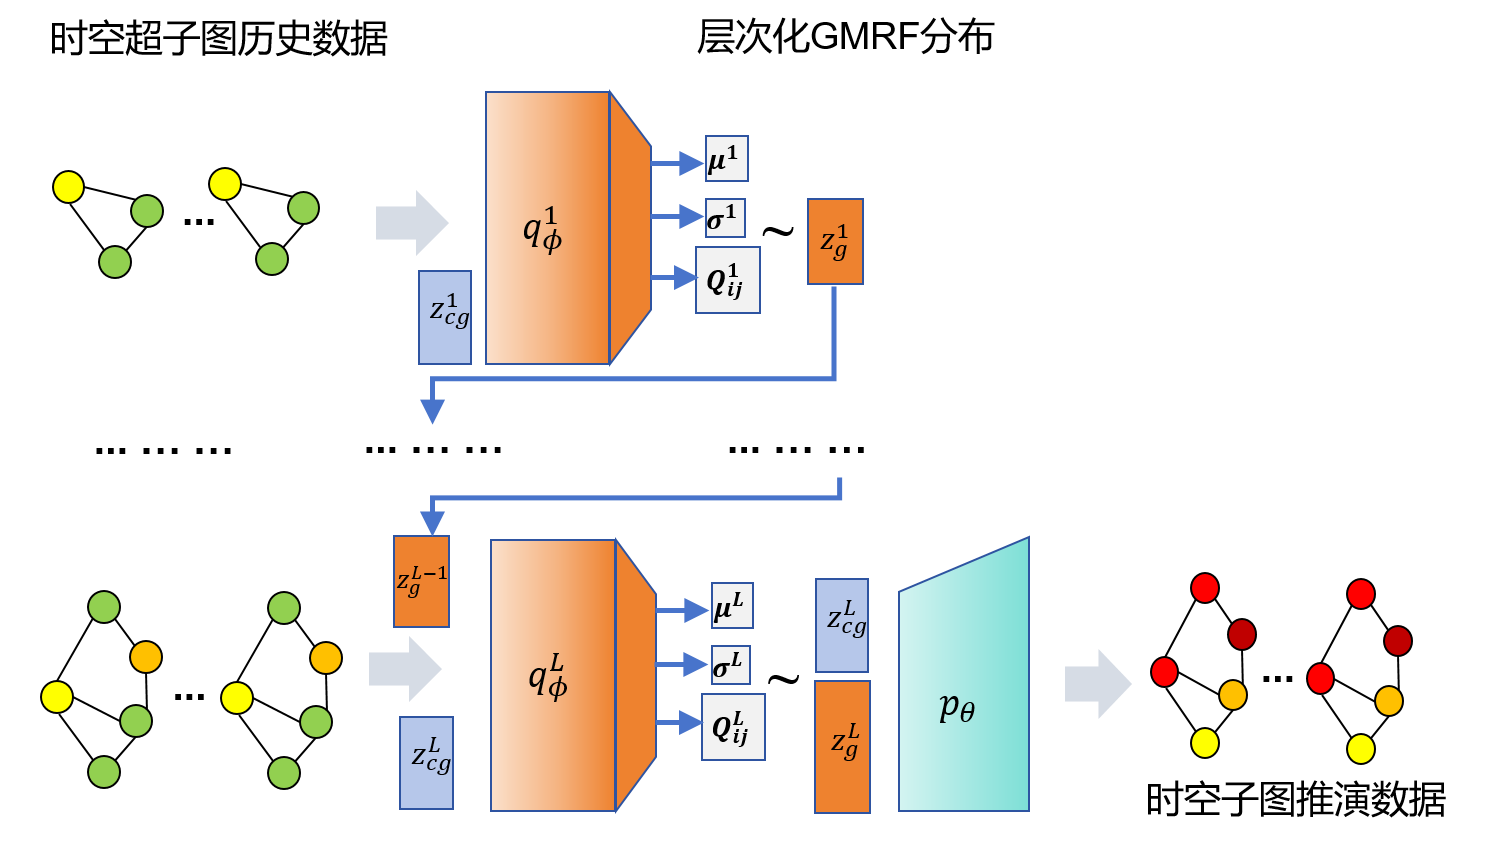
\includegraphics[width=1\linewidth]{fig/gmrf-hvae.png}
    \caption{本研究提出的高斯马尔可夫随机场层次化子图生成模型结构示意图}
    \label{fig:gmrf-hvae}
\end{figure}
%对于不同层之间的模型,我们则采取参数复用的方法。由于不同层的模型间具有全序关系,我们可以自顶向下地对模型进行训练,并利用上层模型的参数来初始化下层模型,以达到快速收敛的目标。根据层次化划分的原则,

本课题将就以上模型设计中的具体实现以及模块的具体技术选择进行研究,分析其性能,并设计合理的训练方法。

\textbf{(3)层次化样本构建和采样策略。}基于上述模型架构,我们需要对训练样本进行构建,并设计训练中的样本采样策略。和3.1.2中的基本步骤一致,我们选取每个子图$\mathcal{G}^{L}_g$,并将其周围的事件与其配对,获取联合嵌入表征。当一个子图被选中进入训练流程时,我们需要对一个三维空间上的样本进行多步骤构建来配合对其的训练。图~\ref{fig:xxx}给出了这一采样过程的示意图。

\underline{首先},每个子图的周边子图需要被选入,来帮助学习本层子图之间的空间相关性。我们将$\mathcal{G}^{L}_g$的邻居子图进行采样,并采取3.1.2中介绍的重要性采样等方法提高样本分布的多样性。\underline{其次},$\mathcal{G}^{L}_g$的父超子图$\mathcal{G}^{L-1}_g$需要被选入,来获取上一层数据的分布信息并训练相应的编码器。由于$\mathcal{G}^{L-1}_g$的隐变量估计需要其邻居子图的信息,我们需要对$\mathcal{G}^{L-1}_g$周边的邻居子图也进行采样。\underline{最后},我们重复上述步骤,递归地对更高层$\mathcal{G}^{L}_g$的祖先超子图及其邻居超子图进行采样,获取相应的数据,直至采样到最高层的宏观子图。以上步骤完成了对一个子图$\mathcal{G}^{L}_g$及其相关联的所有层次的超子图的训练样本构建。本课题拟对具体的样本生成和采样算法进行设计,并分析其复杂度和统计合理性。

\subsubsection{3.1.4 基于知识迁移的时空泛化性增强策略}
针对时空事件和样本的稀疏性,本课题拟提出两种应对方案,即基于子图元学习的知识迁移方法,和基于子图原型网络的生成方法。具体研究思路详述如下。

\textbf{(1)基于子图元学习的知识迁移方法}。  
由于时空异质性和样本稀疏性的原因,一个全局的子图生成模型在部分地区可能会具有较大的误差。我们利用元学习的思路,训练一个全局元生成模型$M_\theta$,并学习一个适应性优化的策略,针对数据样本较少的子图,通过对模型$M_\theta$进行适应性优化来获得一个更准确的本地化的模型。以模型无关的元学习(Model-Agnostic Meta-Learning, MAML)方法为例,我们介绍元学习的基本步骤。给定一系列的学习任务$\mathcal{T}_i\in \mathcal{T}$,每个任务包括一个查询集$Q$和一个支持集$S$,其中$Q$和$S$均包含标记过的学习样本。首先,初始化一个元模型$M_\theta$。从任务集合中采样出一批任务$\mathcal{T}_1, \mathcal{T}_2, ... \mathcal{T}_k \in \mathcal{T}$。针对每一个任务$\mathcal{T}_i$,复制当前的元模型$M_\theta$作为初始模型,并在此基础上继续用支持集$S_i$训练针对该任务的模型$M_{\theta_i}$进行一次参数更新(例如梯度下降法)。当所有任务的模型$M_{\theta_i}$更新完毕之后,利用每个任务的查询集$Q_i$对所有任务模型$M_{\theta_i}$进行一次测试,利用所有模型的总损失,对元模型$M_\theta$进行一次参数更新。重复以上包括采样和训练在内的步骤若干次,直到模型收敛为止。这样,我们得到一个具有良好任务泛化性的元模型$M_\theta$。当一个新的任务出现时,我们可以用少量标记过的数据样本对$M_\theta$进行快速适应性优化,得到针对新任务的有效模型。

在本课题中,给定一个预训练或初始化好的子图生成模型$M_\theta$,我们的目的是通过元学习的训练提高$M_\theta$的空间泛化性。按照上述MAML方法的框架,一个简单的思路是将每个子图上的生成定义为一个任务,将数据按不同事件段分割成查询集和支持集。基于元学习的策略,我们可以为每一个子图学习一个本地模型$M_{\theta_i}$。然而,由于每个子图上的数据量不同,部分任务的训练会较为困难,也会导致全局元模型的参数被样本多的地区影响。

针对这个障碍,本课题提出对子图进行动态聚类的思路,将其划分为子图群。其目的是将环境类似,条件生成模式和规律接近的子图放入一个任务中,以达到较好的泛化性。根据3.1.3中子图划分方式的思路,每个子图对应一个超图结构$G^S$上的超节点,每个子图群则对应超图上的一个子图$G^S_i$,即我们相当于在之前得到的超图结构$G^S$上进行一次新的超子图划分。这里的划分思路与之前的子图划分有所不同。首先,每个划分出的超子图$G^S_i$均不重叠,即每个原图中的子图$G_g$只属于一个子图群。其次,每个超子图的大小不固定。最后,划分的依据不再是子图内数据的相关性,而是在生成模型$M_\theta$在各个子图上表现的均一性。

图群划分是一个具有挑战性的任务。由于划分效果的评价指标依赖于生成模型的最终表现,我们难以设计一个最优算法对子图群进行提前划分。故而,本课题提出将划分和元学习融为一体,形成一个闭环,通过元学习的模型误差来进行超子图的划分。具体思路如下:

(1)首先建立$P$个空的超子图。然后通过随机采样的方式在$G^S$上选取$P$个初始超节点。通过对每个超节点对应的子图进行数据采样,形成$P$个子图数据生成任务$\mathcal{T}_1, ... \mathcal{T}_P$。

(2)然后,利用当前元模型$M_\theta$对这$P$个任务的具体模型进行初始化,并利用其支持集数据对$P$个本地模型进行参数更新。

(3)不同于MAML算法,这里我们进行一次超子图扩展,从$P$个超子图中随机选出$m$个,$\mathcal{T}_1, ... \mathcal{T}_m$。针对每个被选中的超子图$\mathcal{T}_i$,我们从$\mathcal{T}_i$周边邻接且未分配的超节点中选取一个加入$\mathcal{T}_i$。选取的方法是用$\mathcal{T}_i$的本地模型$M_{\theta_i}$对每个待选超节点上的支持集数据进行一次生成,并选取损失函数值最小的一个节点加入。

(4)然后,我们再对本地模型进行一次更新,用所有目前在超子图内的节点的支持集进行采样后更新一次本地模型参数。最后,当所有本地模型完成这次更新后,我们用每个超子图内所有节点的查询集进行一次生成,并利用其总损失函数更新全局模型。

(5)我们重复步骤(2)-(4),对现有的超子图再次进行随机挑选并扩展,直到达到最大步数或者全局模型收敛到指定误差范围。最终我们获得$P$个超子图划分,以及一个元模型。

当有新的子图数据生成任务时,如果目标子图有查询集数据,我们可以使用子图所在的子图群模型,加上样本数据进行微调得到新的模型。如果目标子图没有查询集数据,则我们可直接使用其所在图群的生成模型进行数据生成。图~\ref{fig:}给出了以上过程的示意图。

上述学习过程的一个关键问题是如何从$P$个任务中选出$m$个进行扩展,并保证每个任务都被选中过。这里我们可以采用动态重要性采样(importance sampling)的方法,动态调整每个子图的被选概率。例如,当一个任务刚刚扩展过之后,可以将其被选中概率降低;如果一个任务扩展后的整体损失函数值增大,则表明该任务内的时空异质性开始增大,我们同样可以将其被选中的概率降低。相对地,尚未被选中的任务和内部异质性较低的任务则会获得更大的概率。

另外,如何高效地进行上述模型训练也是一个需要深入研究的问题。本课题拟对以上两个重要问题进行进一步研究,设计合理有效的任务选取策略和计算上高效的元模型训练算法。

\textbf{(2)基于原型网络的零样本子图生成策略}。在一些时空图数据生成场景中,局部地区可能没有任何可供训练的时空事件。例如,在一个从未举办过大型活动的区域推演举办大型演唱会时的交通流量。根据之前阐述的采样方法,当一个子图附近没有任何事件的时候,我们可以将该地区的数据与距离较远的事件配对作为训练样本。这种情况下,由于事件对该地区几乎没有影响,所以相当于一个无条件生成的样本。这导致模型难以学到时空事件对其的真正影响。

零样本学习也是机器学习当中一个重要的研究方向。其中一类零样或少样本学习方法称为原型学习(prototype learning),即学习一系列具有代表性的输入样本的特征(称为原型,prototype)。当一个新的没有任何训练样本的任务来到时,可以将输入的测试样本与学习到的原型特征进行比对,并根据相似性来选取原型特征对应的模型输出来完成对新任务的预测或生成。为了阐述具体研究策略,我们先简单介绍一种原型网络的实现架构。图~\ref{fig:proto-graph}给出了一种深度原型网络的结构。样本经过输入,首先经过一个编码器进行特征提取。之后,提取过的特征向量通过原型层(Prototype Layer)。原型层中的每个节点代表一个参数化可训练的原型特征,表示为一个向量。输入样本的特征向量与每个原型进行相似度计算,得到相似分数向量。最后,该相似分数向量通过一个全连接层,最终产生输出(例如分类或回归的预测值)。设计原型网络需要攻克两个技术难点:(1)如何设计输入样本与原型之间的多维相似性度量,以及(2)如何对网络进行训练来学习到多样化、具有代表性的原型,避免其高度同质化。现有的原型网络学习方法在图片分类、语音识别、自然语言分析等领域有较广泛的应用,但在时空数据上的应用极少。时空数据尤其是图数据的相似度度量以及训练方法与以上几类应用相比具有独特性,因而无法直接应用已有的原型网络模型进行训练。
\begin{figure}
    \centering
    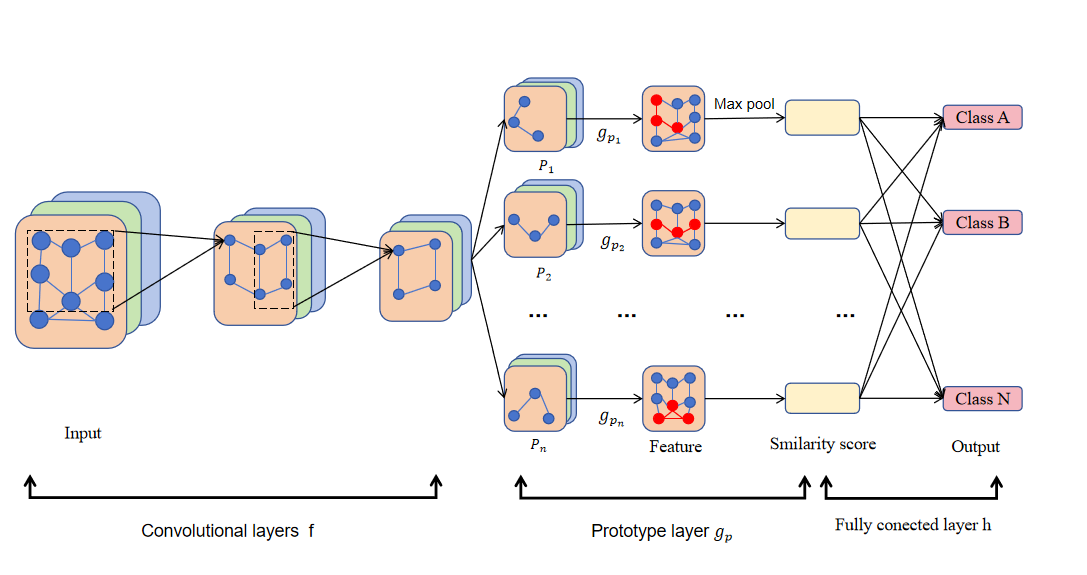
\includegraphics[width=0.9\linewidth]{fig/proto-graph-new.png}
    \caption{图结构分类问题上的一种原型网络结构实现}
    \label{fig:proto-graph}
\end{figure}
在本课题中,我们利用原型网络学习的方法,对子图生成模型进行增强。这一设计的动机是将输入信息与模型学习到的信息相匹配。例如,当一个街区的路段上需要进行交通事故条件下流量推演的时候,模型可能会倾向于选择类似路网结构的原型、同样包含与交通事故信息类似的原型、以及交通数据分布和输入街区类似的原型来拟合出相应的输出。具体地,每一个输入样本为一个时空子图$、\mathcal{G}_g$及其历史数据${X}_{gT}$以及周边的事件$c$的嵌入向量$z_c$。%我们希望通过原型网络给出一个隐变量值$z$,对相应的事件后子图数据$X$进行生成。对应的输出为事件$c$发生后的图数据序列$X_g$。我们有一个已经训练过的生成模型$M$,例如3.1.3中介绍的自相关的子图生成模型。
首先,我们设计一个编码器对数据进行信息提取,包括时空图数据信息、时空节点几何信息、事件信息三类。%其中时空事件信息依照3.1.2中介绍的嵌入方法,已经表示为长度$(3\times m+2\times L)\times T$的向量,包括几何影响力嵌入($m$个高斯核函数在$T$个时间步的位置、带宽和2个$L$步广度优先游走的影响力函数)。
我们用时空图卷积操作来对数据$X_{gT}$进行嵌入,得到表征向量$e_1$来表示当前子图的历史数据信息和图结构;用图卷积和位置编码的方法对每个节点的几何属性进行嵌入得到表征$e_2$;再加上之前获得的事件表征$z_c$。将三个表征向量拼接,我们得到了一个$d_p$维的向量:
\begin{equation}
    e = e_1 || e_2 || z_c \in \mathbb{R}^{d_p}
\end{equation}
网络的下一层是原型层,每个原型$p_i$是长度为$d_p$的可学习参数化向量。原型向量的数量是一个可以调整的超参数。定义一个相似度函数$sim(): \mathbb{R}^{d_p} \times \mathbb{R}^{d_p} \rightarrow \mathbb{R} \in [0,1]$,我们可以计算$e$与每个原型$p_i$之间的相似度$sim(e, p_i)$,得到$d_p$维的相似度向量$S$。最后,将相似度向量通过一个全连接网络,产生输出变量值。

该原型网络模块可以嵌入到3.1.3章节中介绍的基于高斯马尔可夫随机场的生成模型中,作为编码器,训练模型对精度矩阵$Q$的生成。当时空图局部缺乏事件样本时,我们可以通过原型网络拟合出$Q$矩阵的相应列,帮助模型学习到如何更精准地拟合GMRF分布。%;该模块也可以直接对隐变量$z$进行输出,从而直接获得对$X$的预测值。这种方法相当于直接对$X$进行预测,将使结果失去统计的随机性和多样性。

设计这个模型需要解决上述的两个重要问题,即相似度度量和训练方法。针对第一个问题,常见的相似度度量包括欧氏距离和余弦相似度。由于本课题中设计的嵌入向量具有明确的时空含义,这两种相似度的度量无法完全刻画输入样本与原型之间在时空上的相似程度。相应地,我们提出一种新的时空相似度度量,即


针对第二个问题,即训练策略问题,我们添加相关的损失函数项来引导模型学习到差异化较大的原型。这也是相关方法常用的训练策略。具体地,我们为损失函数添加一个多样性(diversity)项,来增加不同的原型之间的差异:
\begin{equation}
    \mathcal{L}_{Div} = \sigma(\min_{i\ne j} -sim(p_i, p_j)),
\end{equation}
其中$sim()$为相似度度量函数,$\sigma$为Sigmoid函数,将取值范围归一化到0到1之间。该项值随着原型之间差异增大而减小,即降低损失函数值。故而鼓励模型学习到差异性大的原型。

%除此之外,我们还需要引导模型学习到地理位置分散的原型。这是因为如果原型都来自于同一个区域,则
最终,总的损失函数由公式~\ref{eq:proto_loss}给出。其中$\mathcal{L}_M$为原始模型$M$的损失函数,例如公式~\ref{eq:gmrf_loss}给出的GraphVAE损失函数。$\lambda$为超参数。
\begin{equation}
    \mathcal{L} = \mathcal{L}_M + \lambda_1\mathcal{L}_{Div}
    \label{eq:proto_loss}
\end{equation}

本课题将对如何具体实现原型网络,以及如何将其与前文介绍的基于GRMF的子图生成模型进行融合进行深入研究。同时将考察不同相似性度量对模型效能的影响。

\textbf{基于代理人模型仿真的数据增强:}除了用机器学习的方法训练模型增加迁移性,我们还可以通过仿真的方式对数据进行增强。例如,在路网交通流量推演的应用场景中,我们可以使用常见的交通模拟器例如Sumo\footnote{https://eclipse.dev/sumo/}对城市交通事件进行仿真,并获得相应的车流量数据统计值。在相关的研究中,申请人团队曾多次应用仿真模型对时空事件挖掘、交通流量预测等问题进行数据增强。%\footnote{Vahedian et al. A traffic flow approach to early detection of gathering events: Comprehensive results. ACM Transactions on Intelligent Systems and Technology (TIST) 8.6 (2017): 1-24.}。
例如,通过获取轨迹数据等辅助信息,我们可以对大型事件前后交通进行分析,并获得出发地、目的地、出发时间、到达时间等参数随时间的变化的分布。图~\ref{fig:event-simu}给出了申请人前期工作中~\footnote{\footnotesize Vahedian et al. A traffic flow approach to early detection of gathering events: Comprehensive results. ACM Transactions on Intelligent Systems and Technology (TIST) 8.6 (2017): 1-24.}由出租车轨迹数据分析获得的一场大型演唱会开始前所有出租车的到达时间分布图。根据类似分析获得的参数,我们可以对其他类似事件的交通流量进行仿真,获得符合交通规律的事件条件下路网车流量、车流速度等信息。同时,研究团队计划和交通领域的相关专家合作(目前已开展),利用交通领域的专业知识进行数据增强方法的合作研究。这些方法可以为本课题提出的数据驱动的推演方法提供验证和补充,促进技术完善并落地。
\begin{figure}
    \centering
    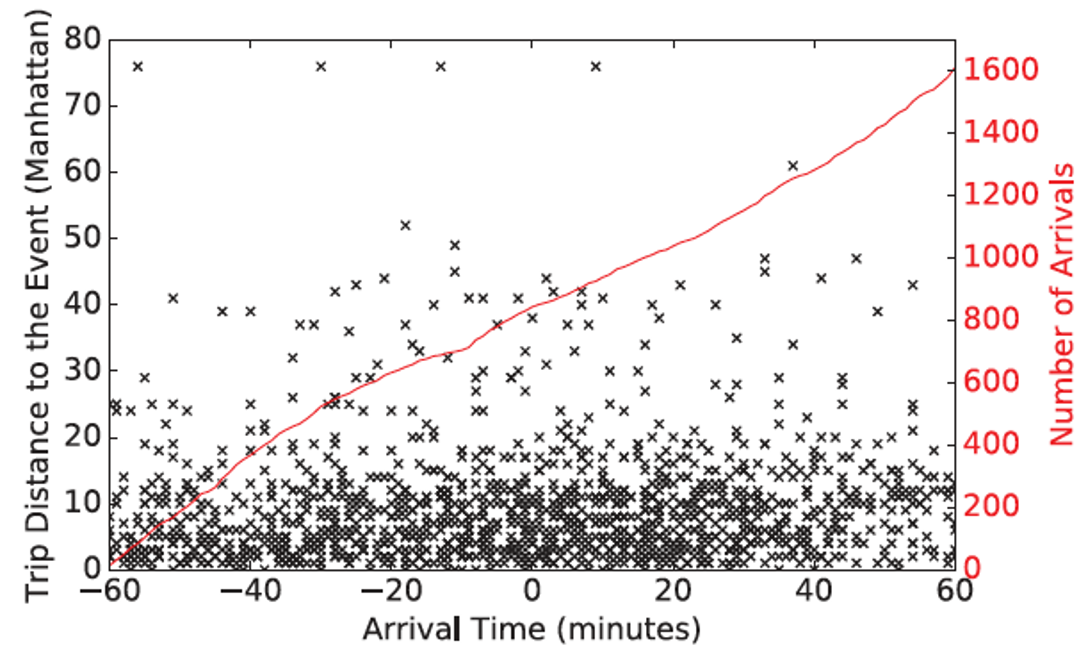
\includegraphics[width=0.5\linewidth]{fig/event_simu.png}
    \caption{某城市聚集事件中出租车到达时间与距离关系分析}
    \label{fig:event-simu}
\end{figure}

\subsection{3.2 可行性分析}
本课题围绕``多维度事件条件下自相关子图生成式推演技术''这一具有重要应用价值的时空数据挖掘问题进行研究。所提出的子问题均针对如何解决这一总体问题的具体挑战。首先,通过时空事件的多层次建模和表征学习,将时空上维度各异、语义上内容多样的时空事件进行归一化的特征提取,为设计相关的生成式学习技术扫清了障碍。其次,通过提出子图生成这一新的方式,克服了现有图数据生成中一次性生成或顺序生成方式的难以训练、误差积累等缺点,并提出了相应的子图样本生成策略。针对子图生成中的样本时空自相关性,本课题创新性地提出了基于高斯马尔科夫随机场隐变量空间的子图生成策略。该技术将高斯马尔可夫随机场和深度图生成模型结合,提供了一种对时空自相关性的显式学习方法,有效地支持了课题提出的子图生成策略。针对样本的时空异质性挑战,本课题进而提出了基于时空子图元学习的策略来提高模型的知识迁移能力。通过动态地划分子图群,将全局模型适应性优化到整个时空图的不同局部,进一步支持了时空图推演的生成质量。最后,针对时空事件样本的稀疏性,提出了基于时空原型网络的零样本学习方法以及基于仿真的数据增强策略,进一步提高了子图生成模型的时空泛化性。本课题还将搭建事件条件下的子图生成式推演实验和展示系统,将上述技术有机地结合起来。因此,本课题的研究问题清晰,各部分之间逻辑清晰且互成体系,总体研究策略和路线是明确的、合理的。

针对本课题提出的创新技术,申请人及主要研究者团队前期进行了相关的研究,并积累了充分的经验和成果,为本课题的研究奠定了基础。具体包括:

(1)在时空数据的生成式学习上,研究团队在交通数据上提出了一系列的基础生成模型,例如基于GAN模型的交通流量数据生成学习方法,通过时空划分对局部张量进行条件生成。相关成果发表在KDD,WWW,ICLR,ICDM,SDM等重要数据挖掘和机器学习会议中。其中STORM-GAN是一种基于栅格数据的条件生成网络,将疫情防控措施作为生成条件,对多城市的人口移动模式进行生成式学习。图~\ref{fig:storm-gan-net}和图~\ref{fig:storm-gan}展示了STORM-GAN的架构,及其在美国休斯顿数据上的生成的结果(多次生成样本的平均值)与相关基线工作的对比。该工作入选ICDM'22最佳论文候选。本课题将在相关研究的基础上,融合相关模型的设计思想,对子图生成技术进行研究。
\begin{figure}
    \centering
    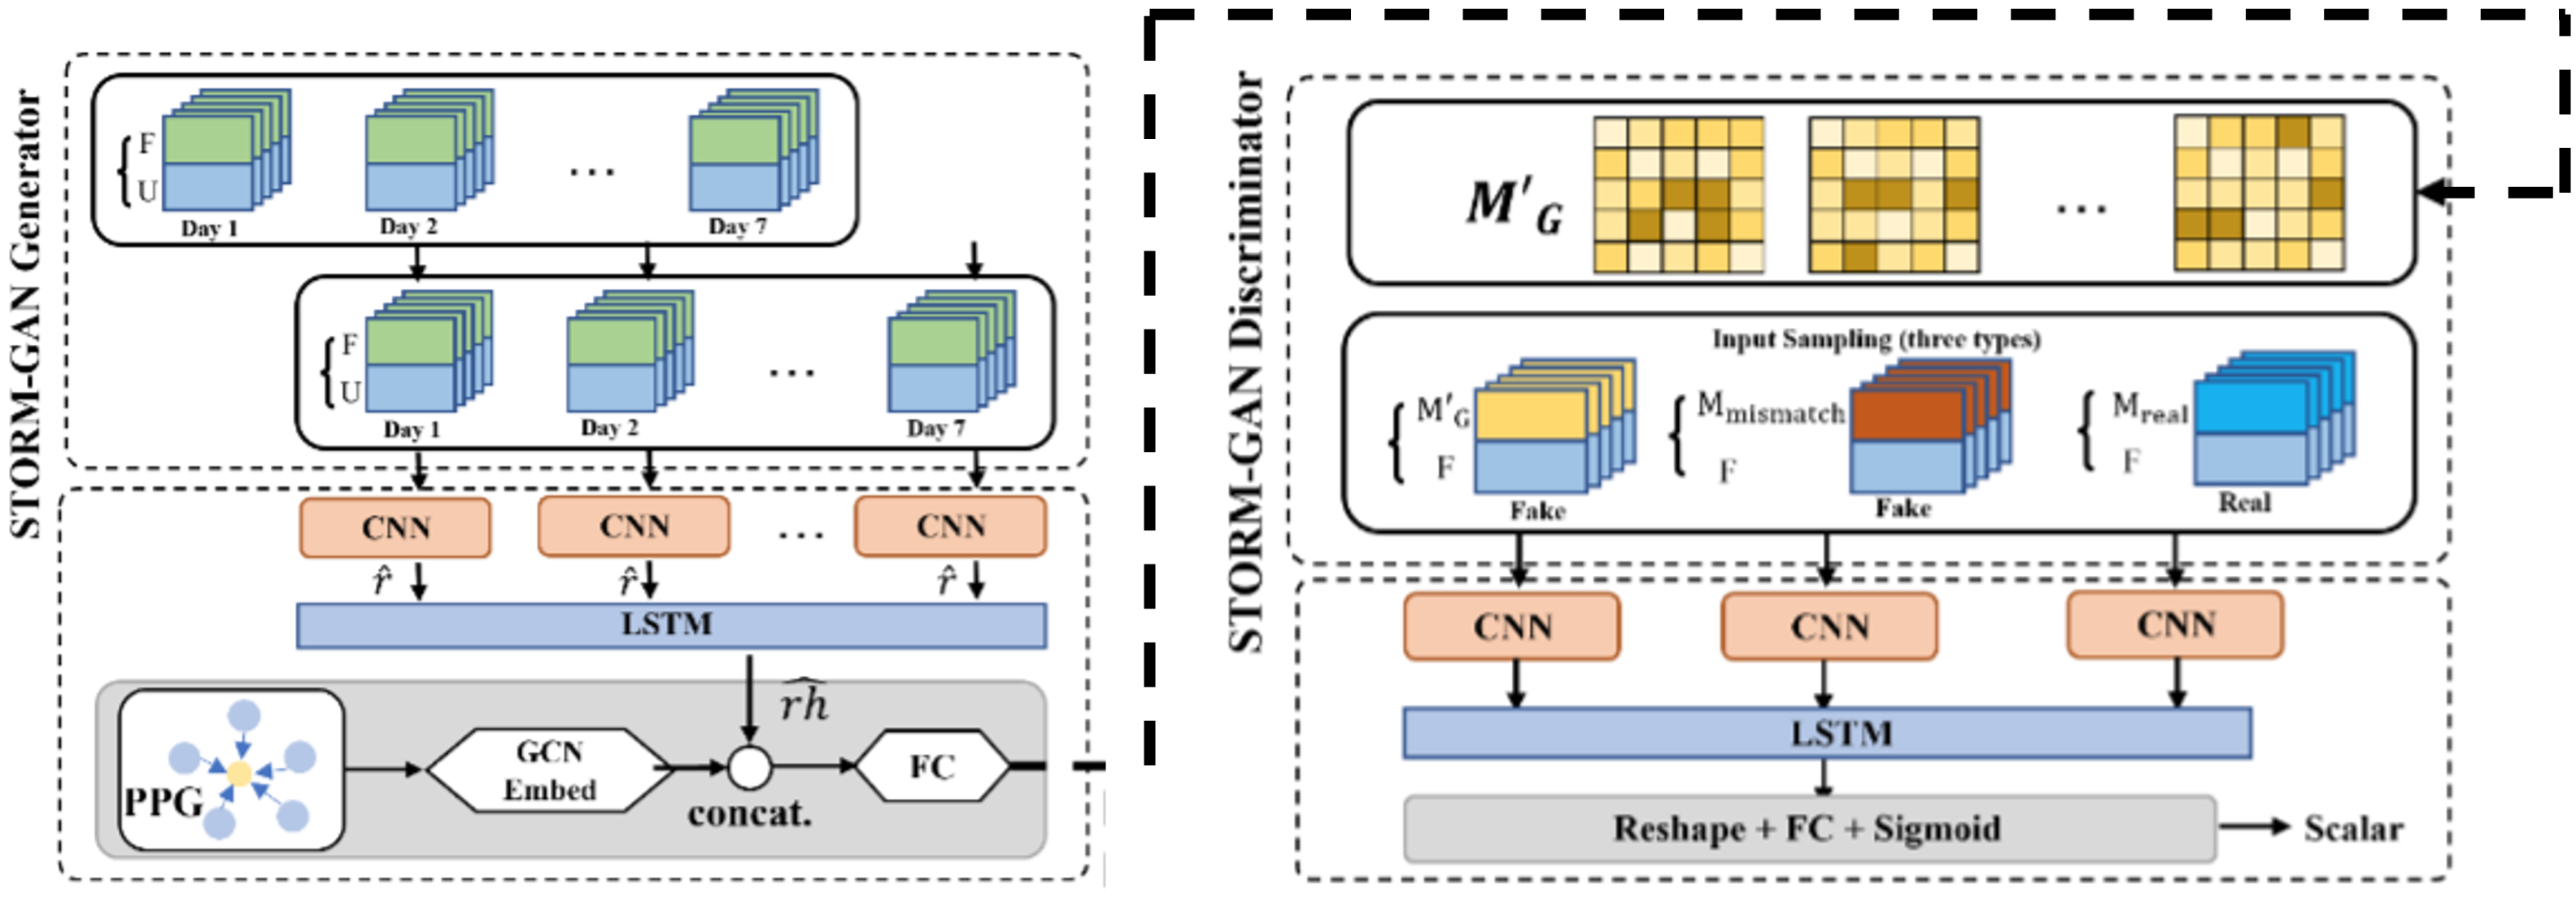
\includegraphics[width=0.9\linewidth]{fig/storm-gan-network.png}
    \caption{STOMR-GAN生成网络结构}
    \label{fig:storm-gan-net}
\end{figure}
\begin{figure}[h]
    \centering
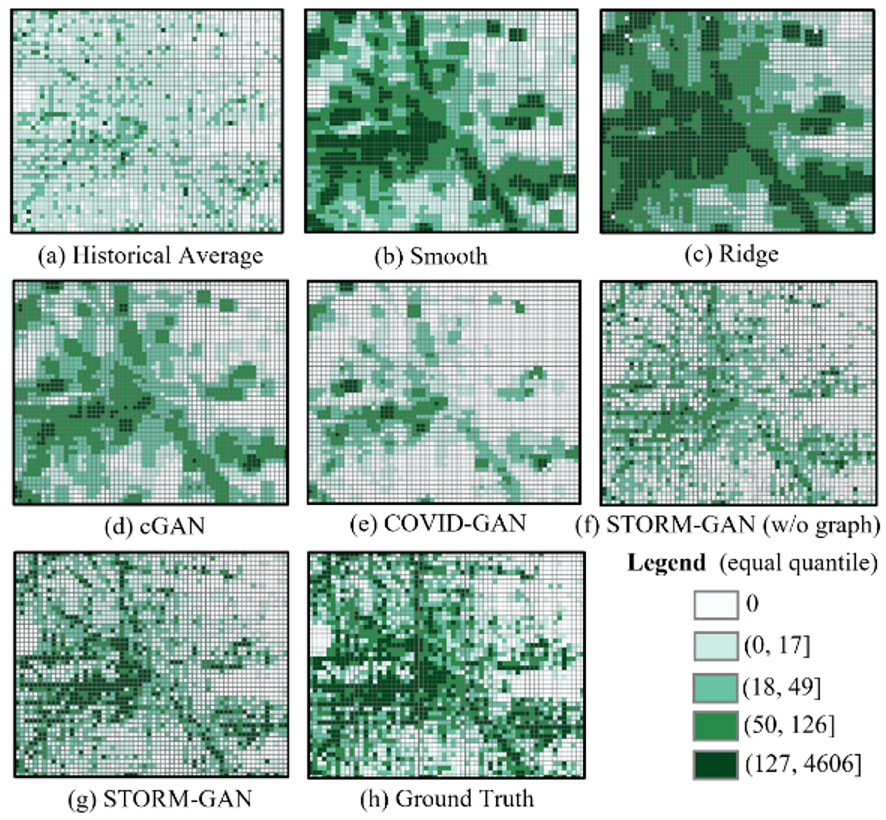
\includegraphics[width=0.7\linewidth]{fig/storm-gan.png}
    \caption{申请人在栅格时空数据上提出的条件生成模型STORM-GAN结果展示}
    \label{fig:storm-gan}
\end{figure}

(2)自相关性和异质性时空数据挖掘方面,申请人及主要研究者团队提出了基于相关性采样的事件预测模型SpatialRank(NeurIPS'23),基于空间划分和空间集成学习的异质性数据预测模型Hetero-ConvLSTM和HintNet(KDD'18, SDM'23),以及基于空间知识转移和元学习的异质性数据预测方法(ICDM'21最佳论文奖,KAIS专刊)等。这些相关研究为本课题的子图采样、相关性建模和异质性子图学习模型奠定了技术基础,将有力地支撑本课题的相关研究。

(3)在时空事件建模和预测方面,申请人先后提出了基于时空子图挖掘的城市聚集事件检测和预测方法(SIGSPATIAL)、基于轨迹目的地预测的城市聚集事件预测(SIGSPATIAL, TKDE),和基于生存分析的城市扩散事件预测(AAAI'19)。图~\ref{fig:event-big}给出了对城市聚集事件的形式化刻画与挖掘结果示例。该方法提出将时空事件的动态足迹进行刻画的思路,并设计了高效的时空事件足迹挖掘算法。相关研究对本问题中时空事件的形式化刻画和建模提供了重要思路和借鉴。
\begin{figure*}[b!]
    \centering
    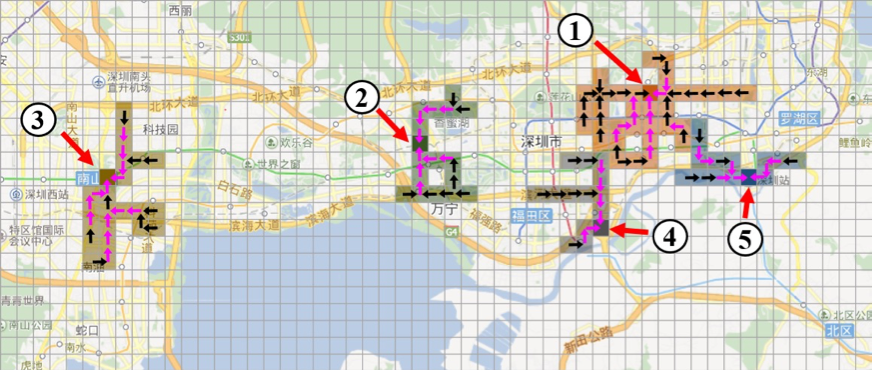
\includegraphics[width=0.9\linewidth]{fig/event_all5.png}
    \caption{申请人工作对时空聚集事件足迹的有向图刻画方法和挖掘结果}
    \label{fig:event-big}
\end{figure*}

综上,本课题所提出的问题和解决方案具有坚实的研究基础,团队具有相关研究经验和成果积累,保证了课题的可行性。此外,研究团队与国内外交通、环境领域的专家建立了良好的合作关系,通过跨学科合作,可以推动本课题的研究成果在不同领域的应用和落地,提高本课题的影响力和实际价值。

\newpage
{\sihao \color{MsBlue} \kaishu 4.{\bfseries 本项目的特色与创新之处;}}

本项目针对时空属性图的条件推演提出一套从建模到表征学习再到预测模型和算法的完整技术框架。针对时空事件属性种类复杂多样且分布稀疏、时空属性图不同子图间的强自相关性和异质性等挑战,本课题提出了一系列创新性的解决思路。项目的特色与创新指出可以概括如下:

(1)本项目的研究对象是时空属性图,但研究内容不同于近年来受到大量关注的一般预测问题,而是聚焦于具有重要现实价值却更具挑战的\textbf{基于非规律性事件的条件式推演问题}。该问题的目标是学习在事件发生的条件下,时空图相关区域的数据分布,从而对数据进行条件式生成。目前,相关研究中尚无解决类似问题的成熟方法。针对时空事件复杂多样的空间几何特征和时空影响力这一挑战,本项目提出了\underline{基于几何特征和图拓扑特征双层建模的思路},并基于该思路提出了对事件信息进行\underline{联合表征学习的技术路线}。这是本项目的第一个创新之处。

%(2)本项目所提出的\textbf{基于图划分的子图生成学习策略}也与已有的图数据生成学习技术路线有明显的区别。已有图生成学习方法一般采用一次性生成或顺序生成的方法对目标图的拓扑或者属性进行生成。根据前文的分析,这两种生成策略在规模较大的时空属性图上都具有明显的缺点。本课题提出的生成策略聚焦于对每个局部子图的生成学习问题,并设计了\underline{自相关子图生成}和\underline{层次化子图生成}两种子图生成策略,可提高生成的效率和准确性。这是本项目的第二个创新之处。

(2)本项目提出的\textbf{子图样本非独立随机分布假设下的生成策略}是一个新研究思路。目前图数据生成学习技术常遵循的假设是图样本隐变量服从独立随机同分布,例如标准高斯分布。在时空图数据的局部生成问题中,作为样本的子图之间存在天然的空间自相关性,而非独立随机关系。相应地,代表样本中不同维度特征的隐变量也应符合自相关性的约束。针对这一观察,本课题创新性地提出了\underline{基于自相关性隐变量的技术路线},将子图表示为超节点,将有向图转化为聚集的层次化无向图,进而用条件随机场等模型进行求解。通过对条件随机场进行联合采样来进行自相关的数据生成。这一技术路线是本项目的第二个创新之处。

(3)本项目提出的\textbf{层次化自相关子图生成策略}是对多尺度时空子图生成技术的创新。自相关的时空子图生针对尺度较小的生成任务会出现额外生成数据的低效率情况,同时生成方式不够灵活,无法满足多尺度推演的需求。针对这一观察,本课题创新性地提出了\underline{层次化的自相关子图生成方法},通过将时空图转化为层次化无向超图并学习层间子图依赖关系建立自顶向下的生成模型。这一技术路线是本项目的第三个创新之处。

(4)本项目提出了\textbf{基于局部知识迁移的时空泛化性增强策略}。由于时空图不同区域存在明显的时空异质性,一个全局模型通常无法准确刻画各个局部子图的数据分布。同时,时空事件的稀疏性和不均分布导致部分区域的训练样本较少。因此,在子图生成时,模型的时空泛化性是一个重要挑战。%这一问题在时空图数据预测和生成学习中均较少被关注。
本项目提出了基于\underline{时空子图元学习}和基于\underline{时空原型学习}的训练策略来增强模型时空泛化性,是本项目的第四个创新之处。
\newpage
{\sihao \color{MsBlue} \kaishu 5.{\bfseries 年度研究计划及预期研究结果}(包括拟组织的重要学术交流活动、国际合作与交流计划等)。}
\subsection{5.1 年度研究计划}
本项目的研究期限为2025年1月至2028年12月。具体工作安排如下:
%拟组织研讨会1次,将这个模版广而告之。但是目前还没有经费。
%
\begin{table*}[h!]
    \centering
    \begin{tabular}{|p{2.5cm}|p{11.5cm}|}
        \hline
        时间 & 研究工作内容\\\hline
        2025年1月 - 2025年12月 & 研究时空属性图和时空事件的形式化建模与刻画方法,研究时空事件与时空图联合表征学习理论、模型结构和算法。构建时空图数据推演的实验平台和数据集,将上述模型和算法在实验平台上进行验证。撰写科学论文2-3篇。\\\hline
        2026年1月 - 2026年12月 & 研究基于隐变量自相关假设的时空子图生数据成策略,设计时空子图划分的算法、自相关子图数据采样算法,研究基于高斯马尔可夫随机场隐变量空间的数据生成理论、模型、算法。将上述研究成果加入实验平台并进行验证。撰写相关学术论文3-4篇,申请相关专利1项,组织时空数据生成式学习和时空图数据挖掘相关研讨会一次。\\\hline
         2027年1月 - 2027年12月& 研究时空属性图上层次化子图生成的相关技术。设计层次化子图划分策略和算法,研究层次化时空子图生成学习的样本构建策略,研究层次化时空子图数据生成学习的理论、模型、算法。将上述研究结果集成到实验平台并进行验证。撰写学术论文2-3篇,申请专利1项,组织时空数据生成式学习方面的研讨会一次。\\\hline
         2028年1月 - 2028年12月& 研究基于局部知识迁移的时空泛化性增强策略。设计时空子图元学习的理论、模型、算法,研究时空子图原型网络的设计方案、模型、训练算法,实现时空子图生成模型的知识迁移,增强模型泛化性。与设计基于代理人模型仿真的时空属性图数据增强方法。将上述研究结果加入到实验平台中,并进行结果验证。撰写相关学术论文2-3篇。整理课题研究的相关资料、已发表研究成果,撰写项目总结报告。组织时空数据生成式学习研讨会一次。\\\hline
    \end{tabular}
    %\caption{Caption}
    \label{tab:timeline}
\end{table*}
\vskip -5mm %可以通过类似的命令微调行距以使得排版美观

\subsection{5.2 预期研究结果}
基于所研究的成果,本课题预期将在国内外高水平国际学术会议和重要学术期刊上
发表论文10-12篇;设计并实现一个基于时空属性图的条件式推演的实验和原型展示平台;申请专利1-2项;培养硕士和博士研究生10-12名。
%{\color{MsBlue} \subsection{\sihao \kaishu \quad \ (二)研究基础与工作条件 }}


{\sihao \color{MsBlue} \kaishu 1.{\bfseries 研究基础}(与本项目相关的研究工作积累和已取得的研究工作成绩);}

本课题的主要研究人员长期致力于时空数据挖掘、分析、智能技术的研究工作,尤其在时空事件分析挖掘、时空图数据挖掘、时空数据生成式学习等具体领域具有较为丰富的研究经验,对国内外研究进展和现状有全面的了解把握,相关研究成果已发表在重要的国际会议和期刊中,包括IEEE Transactions on Knowledge and Data Engienering (TKDE),International Journal on Geographical Information Sciences (IJGIS)(地理信息系统领域顶级期刊),KDD, NeurIPS,AAAI,ICDE,WWW,ICLR等,并多次获得最佳/优秀论文奖。

项目负责人周逊目前为哈尔滨工业大学(深圳)三级教授、博士生导师,曾任美国爱荷华大学商业分析系(信息系统方向)终身副教授,系博士项目主任,并双聘于爱荷华大学应用与计算数学和信息学两个系任博士生导师。长期致力于时空数据挖掘、时空大数据分析、时空计算等领域的研究,攻读博士学位期间师从国际知名时空数据挖掘和时空数据库专家,明尼苏达大学Shashi Shekhar教授(IEEE和AAAS Fellow)。2016年获得美国国家科学基金NSF CRII奖(被名校广泛认为是计算机领域的pre-CAREER奖)。目前为IEEE高级会员,并入选国家优青(海外)人才项目。在数据挖掘、机器学习和时空计算等相关领域的会议和期刊上发表论文100余篇,包括议KDD,AAAI,NeurIPS,WWW,CIKM,ICDM,SDM,TKDE,KAIS,Geoinformatica等CCF-A/B类会议和期刊40余篇,其他JCR Q1期刊20余篇,获得包括ICDM'21 Best Paper Award, SDM'19 Best Applied Data Science Paper在内的5次国际国内一流会议最佳或优秀论文奖。联合主编Springer出版的地理信息系统大百科全书一部。在美期间承担了美国国家科学基金NSF、美国交通部、爱荷华大学等机构资助的7项与时空大数据分析、挖掘与智能相关的研究项目。

针对本项目的研究内容,申请人及研究团队成员具有较为丰富的相关研究经验和扎实的研究基础,详述如下:

在时空数据的生成式学习方面,申请人先后提出了基于生成对抗网络GAN的栅格化交通流量数据生成学习方法TrafficGAN~\cite{zhang2019trafficgan-x},CurbGAN~\cite{zhang2020curb-x},Mest-GAN~\cite{zhang2022mest-x},$C^3$-GAN~\cite{zhang2021c-x}等,并提出了基于条件生成学习方法的疫情期间人流量数据生成模型COVID-GAN~\cite{}与STORM-GAN~\cite{}。这些成果均发表于KDD、ICDM、KAIS、SIGSPATIAL、ACM TIST等CCF-A/B类会议、重要时空计算国际会议和JCR Q1类期刊上。其中STORM-GAN入选2022年ICDM(CCF-B类)会议最佳论文候选。所指导的美国爱荷华大学博士生获得学校优秀博士毕业论文资助奖金。%并入选学校Dare to Discover活动作为优秀科研人才被报道。
上述成果使得申请人对时空数据的生成式学习研究有了充足的技术准备,本课题将基于以上研究成果,对时空图结构表示的时空数据上的生成式学习进行深入研究。

在时空事件的分析、挖掘与建模上,申请人团队针对时空聚集事件~\cite{}、时空扩散事件~\cite{}、交通事故与犯罪等点过程事件~\cite{}等多种类时空事件进行了深入研究,提出了对其动态时空足迹进行刻画和挖掘的多种方法。相关工作发表在AAAI, TKDE,SIGSPATIAL等重要会议和期刊上。这些前期成果为本项目中对时空事件进行双层次建模和刻画的任务提供了良好铺垫。

针对时空数据分析中的自相关性和异质性的挑战,申请人提出了一系列基于重要性采样~\cite{}、空间划分~\cite{}、空间集成学习~\cite{}、知识迁移~\cite{}等技术提高预测准确性的方法,并将研究内容应用到交通事故和犯罪事件预测等方面,取得了良好的效果,相关研究获得美国交通部和NVidia公司项目资助。其中一篇研究异质性数据预测的论文获得CCF-B类ICDM'21年度唯一最佳论文奖~\cite{}。这些前期的研究积累为本课题中处理子图生成中的时空自相关性和异质性挑战提供了重要的技术储备和扎实的理论基础。

在时空图数据的分析和挖掘上,申请人提出了基于轨迹数据的时空图可达性分析查询算法~\cite{}。申请人还提出了基于时空有向图挖掘的城市聚集事件监测和预报方法~\cite{}。以上工作均发表在CCF-A类期刊IEEE TKDE上。此外,申请人还提出了基于时空图卷积神经网络的交通事故预测和分析技术~\cite{}和基于图神经网络的视频中物体跟踪分析方法~\cite{}。这些前期研究使团队具备了充分的时空图数据挖掘分析和深度学习的经验和方法积累。

以下为课题主要研究人员已发表的相关论文:
\bibliographystyle{ieeetrNSFC}
\bibliography{mywork}
%申请人用\LaTeX 写过几篇文章,包括自己的博士论文。

{\sihao \color{MsBlue} \kaishu 2.{\bfseries 工作条件}(包括已具备的实验条件,尚缺少的实验条件和拟解决的途径,包括利用国家实验室、国家重点实验室和部门重点实验室等研究基地的计划与落实情况);}

本项目依托单位为哈尔滨工业大学(深圳)。哈尔滨工业大学是我国的知名高等学
院,国家“双一流”重点建设的大学。科研工作和人才培养紧紧围绕国防建设和国民经
济建设,与一批国内知名企业和一些相关的国内外研究机构有稳定的联合、合作与协作
关系。哈尔滨工业大学(深圳)计算机科学与技术学院设有计算机科学与技术国家重点
一级学科,具有学士、硕士、博士学位授予权和博士后流动站。计算机科学与技术学科
在2012 年教育部学科评估中位居全国第四,2017 年被评为“双一流”建设学科和全国第四轮学科评估A 类学科,2018 年入选广东省高水平大学重点建设学科。

申请人所在的哈工大深圳“智能与计算研究院”由特聘校长助理、国家杰青获得者张民教授领导,2023年获批成立深圳市重点实验室,目前有7名国家级青年人才,与海外高水平研究机构和院校建立了长期的学术和交流。课题组已有GPU 服务器集群一套(96 个GPU),另有其它独立CPU/GPU 服务器20余台,能充分保障本项目研究开展的有序进行。

{\sihao \color{MsBlue} \kaishu 3.{\bfseries 正在承担的与本项目相关的科研项目情况}(申请人和主要参与者正在承担的与本项目相关的科研项目情况,包括国家自然科学基金的项目和国家其他科技计划项目,要注明项目的资助机构、项目类别、批准号、项目名称、获资助金额、起止年月、与本项目的关系及负责的内容等);}

无。

{\sihao \color{MsBlue} \kaishu 4.{\bfseries 完成国家自然科学基金项目情况}(对申请人负责的前一个已资助期满的科学基金项目(项目名称及批准号)完成情况、后续研究进展及与本申请项目的关系加以详细说明。另附该项目的研究工作总结摘要(限500字)和相关成果详细目录)。}

无。
%不告诉你。

{\color{MsBlue} \subsection{\sihao \kaishu \quad \ (三)其他需要说明的情况 }}

{\sihao \color{MsBlue} \kaishu 1. 申请人同年申请不同类型的国家自然科学基金项目情况(列明同年申请的其他项目的项目类型、项目名称信息,并说明与本项目之间的区别与联系)。 }

无。

{\sihao \color{MsBlue} \kaishu 2. 具有高级专业技术职务(职称)的申请人或者主要参与者是否存在同年申请或者参与申请国家自然科学基金项目的单位不一致的情况;如存在上述情况,列明所涉及人员的姓名,申请或参与申请的其他项目的项目类型、项目名称、单位名称、上述人员在该项目中是申请人还是参与者,并说明单位不一致原因。}

无。

{\sihao \color{MsBlue} \kaishu 3. 具有高级专业技术职务(职称)的申请人或者主要参与者是否存在与正在承担的国家自然科学基金项目的单位不一致的情况;如存在上述情况,列明所涉及人员的姓名,正在承担项目的批准号、项目类型、项目名称、单位名称、起止年月,并说明单位不一致原因。}

无。

{\sihao \color{MsBlue} \kaishu 4. 其他。}

无。

{\color{MsBlue} \subsection{\sihao \kaishu \quad \ (二)研究基础与工作条件 }}
\begin{bibunit}
{\sihao \color{MsBlue} \kaishu 1.{\bfseries 研究基础}(与本项目相关的研究工作积累和已取得的研究工作成绩);}

本课题的主要研究人员长期致力于时空数据挖掘、分析、智能技术的研究工作,尤其在时空事件分析挖掘、时空图数据挖掘、时空数据生成式学习等具体领域具有较为丰富的研究经验,对国内外研究进展和现状有全面的了解把握,相关研究成果已发表在重要的国际会议和期刊中,包括IEEE Transactions on Knowledge and Data Engienering (TKDE),International Journal on Geographical Information Sciences (IJGIS)(地理信息系统领域顶级期刊),KDD, NeurIPS,AAAI,ICDE,WWW,ICLR等,并多次获得最佳/优秀论文奖。

项目负责人周逊目前为哈尔滨工业大学(深圳)三级教授、博士生导师,曾任美国爱荷华大学商业分析系(信息系统方向)终身副教授,系博士项目主任,并双聘于爱荷华大学应用与计算数学和信息学两个系任博士生导师。长期致力于时空数据挖掘、时空大数据分析、时空计算等领域的研究,攻读博士学位期间师从国际知名时空数据挖掘和时空数据库专家,明尼苏达大学Shashi Shekhar教授(IEEE和AAAS Fellow)。2016年获得美国国家科学基金NSF CRII奖(被名校广泛认为是计算机领域的pre-CAREER奖)。目前为IEEE高级会员,并入选国家优青(海外)人才项目。在数据挖掘、机器学习和时空计算等相关领域的会议和期刊上发表论文100余篇,包括议KDD,AAAI,NeurIPS,WWW,CIKM,ICDM,SDM,TKDE,KAIS,Geoinformatica等CCF-A/B类会议和期刊40余篇,其他JCR Q1期刊20余篇,获得包括ICDM'21 Best Paper Award~\cite{xie2021statistically}, SDM'19 Best Applied Data Science Paper~\cite{pan2019dissecting}在内的5次国际国内会议最佳或优秀论文奖。联合主编Springer出版的地理信息系统大百科全书一部。在美期间承担了美国国家科学基金NSF、美国交通部、爱荷华大学等机构资助的7项与时空大数据分析、挖掘与智能相关的研究项目。

针对本项目的研究内容,申请人及研究团队成员具有较为丰富的相关研究经验和扎实的研究基础,详述如下:

在时空数据的生成式学习方面,申请人团队先后提出了基于生成对抗网络GAN的栅格化交通流量数据生成学习方法TrafficGAN~\cite{zhang2019trafficgan,zhang2020off},CurbGAN~\cite{zhang2020curb},Mest-GAN~\cite{zhang2022mest},$C^3$-GAN~\cite{zhang2021c}等,并提出了基于条件生成学习方法的疫情期间人流量数据生成模型COVID-GAN~\cite{bao2020covid,bao2022covid}与STORM-GAN~\cite{bao2022storm,bao2023storm}。在轨迹数据的生成学习方面提出了基于时空模仿学习的cGAIL~\cite{zhang2020cgail}、TrajGAIL~\cite{zhang2020trajgail}等模型。这些成果均发表于KDD、ICDM、KAIS、SIGSPATIAL、ACM TIST等CCF-A/B类会议、重要时空计算国际会议和JCR Q1类期刊上。其中STORM-GAN入选2022年ICDM(CCF-B类)会议最佳论文候选。%所指导的美国爱荷华大学博士生获得学校优秀博士毕业论文资助奖金。%并入选学校Dare to Discover活动作为优秀科研人才被报道。
团队成员还提出了基于生成模型的出行时间估算方法~\cite{li2019learning}
上述成果使得申请人及团队对时空数据的生成式学习研究有了充足的技术准备,本课题将基于以上研究成果,对时空图结构表示的时空数据上的生成式学习进行深入研究。

在时空事件的分析、挖掘与建模上,申请人团队针对时空聚集事件~\cite{vahedian2017forecasting,zhou2016traffic,khezerlou2017traffic,khezerlou2019forecasting}、时空扩散事件~\cite{vahedian2019predicting,khezerlou2021dilsa+}、交通事故与犯罪等点过程事件~\cite{an2024spatialrank}、交通拥堵事件~\cite{xiong2023detecting}等多种类时空事件进行了深入研究,提出了对其动态时空足迹进行刻画和挖掘的多种方法。相关工作发表在AAAI, TKDE,SIGSPATIAL等重要会议和期刊上。主要研究人员还提出了自相关时间序列分析的方法~\cite{liu2022multivariate}。这些前期成果为本项目中对时空事件进行双层次建模和刻画的任务提供了良好铺垫。

针对时空数据分析中的自相关性和异质性的挑战,申请人提出了一系列基于重要性采样~\cite{an2024spatialrank}、空间划分~\cite{yuan2018hetero,xie2021spatial}、空间集成学习~\cite{xie2022statistically}、知识迁移~\cite{an2022hintnet}等技术提高预测准确性的方法,并将研究内容应用到交通事故和犯罪事件预测等方面,取得了良好的效果,相关研究获得美国交通部和NVidia公司项目资助。其中一篇研究异质性数据预测的论文获得CCF-B类ICDM'21年度唯一最佳论文奖~\cite{xie2021statistically}。这些前期的研究积累为本课题中处理子图生成中的时空自相关性和异质性挑战提供了重要的技术储备和扎实的理论基础。

在时空图数据的分析和挖掘上,申请人提出了基于轨迹数据的时空图可达性分析查询算法~\cite{ding2019mining},发表在CCF-A类期刊IEEE TKDE上。申请人还提出了基于时空有向图挖掘的城市聚集事件监测和预报方法~\cite{zhou2016traffic,khezerlou2017traffic}。此外,申请人还提出了基于时空图卷积神经网络的交通事故预测和分析技术~\cite{an2022hintnet}和基于图神经网络的视频中物体跟踪分析方法~\cite{ding2022egospeed}。主要研究者团队还提出了基于图数据的交通流量预测、路网表示学习等模型~\cite{li2020spatial,guo2021learning,chen2021robust}等。这些前期研究使团队具备了充分的时空图数据挖掘分析和深度学习的经验和方法积累。

以下为课题主要研究人员已发表的相关论文($^\dagger$表示申请人独立指导的研究生,$^{+}$表示申请人作为校外导师联合指导研究生):
\patchcmd{\thebibliography}{\section*{\refname}}{}{}{}
  {\settowidth}
{\setlength{\parsep}{0pt}\setlength{\itemsep}{0pt plus 0.1pt}\settowidth}
  {}{}


%\bibliographystyleMy{ieeetrNSFC}
%bibliographystyleMy{mywork}
{
\small
\putbib[mywork]
}
%申请人用\LaTeX 写过几篇文章,包括自己的博士论文。
\end{bibunit}
{\sihao \color{MsBlue} \kaishu 2.{\bfseries 工作条件}(包括已具备的实验条件,尚缺少的实验条件和拟解决的途径,包括利用国家实验室、国家重点实验室和部门重点实验室等研究基地的计划与落实情况);}

本项目依托单位为哈尔滨工业大学(深圳)。哈尔滨工业大学是我国的知名高等学
院,国家“双一流”重点建设的大学。科研工作和人才培养紧紧围绕国防建设和国民经
济建设,与一批国内知名企业和一些相关的国内外研究机构有稳定的联合、合作与协作
关系。哈尔滨工业大学(深圳)计算机科学与技术学院设有计算机科学与技术国家重点
一级学科,具有学士、硕士、博士学位授予权和博士后流动站。计算机科学与技术学科
在2012 年教育部学科评估中位居全国第四,2017 年被评为“双一流”建设学科和全国第四轮学科评估A 类学科,2018 年入选广东省高水平大学重点建设学科。

申请人所在的哈工大深圳“智能与计算研究院”由特聘校长助理、国家杰青获得者张民教授领导,2023年获批成立深圳市重点实验室,目前有7名国家级青年人才,与海外高水平研究机构和院校建立了长期的学术和交流。课题组已有GPU 服务器集群一套(96 个GPU),另有其它独立CPU/GPU 服务器20余台,能充分保障本项目研究开展的有序进行。

{\sihao \color{MsBlue} \kaishu 3.{\bfseries 正在承担的与本项目相关的科研项目情况}(申请人和主要参与者正在承担的与本项目相关的科研项目情况,包括国家自然科学基金的项目和国家其他科技计划项目,要注明项目的资助机构、项目类别、批准号、项目名称、获资助金额、起止年月、与本项目的关系及负责的内容等);}

申请人周逊目前没有正在执行的与本课题相关的国家级科研项目。申请人入选国家优青(海外)项目,目前尚待批准立项,目前暂无批准号、资助金额信息。

本课题主要参与者李修成目前作为负责人正执行国家自然科学基金青年科学基金项目1项,批准号62206074,执行期为2023-01-01 至 2025-12-31, 总资助额度30万元,来源为国家自然科学基金委。该项目名为:基于群等变性和深度生成模型的时空图挖掘。该项目与本课题有一定相关性,研究对象同样为时空图数据的挖掘和分析问题。但主要研究内容、研究方向、创新点等方面均与本课题有较大区别:
\begin{enumerate}
    \item 首先,\textbf{研究的问题类别不同}。上述项目研究的核心问题是时空图数据的预测和补全问题。而本课题研究的问题是图数据的条件式生成学习问题。根据申请书1.2章节的分析,时空图数据的推演难以用包括上述课题提出的方法在内的预测技术解决。故而两者研究问题的类别不同。

    \item 其次,\textbf{基本假设和研究方向不同}。上述课题探索的一个主要问题是假设数据缺失或时空图的结构部分未知的情况下,如何通过图结构推断等方式补足信息进行数据预测。而本课题中时空图结构和数据已经给定,不存在缺失的情况。而本项目研究的问题是假设一个时空事件发生,会对时空图数据产生何种影响,但上述课题中不涉及时空事件这一概念。故而两个项目的基本假设和研究方向不同。

    \item 最后,\textbf{创新点不同}。(1)本课题的第一个创新点是对不同维度类型的时空事件进行建模并与时空图进行联合表征学习。而上述项目研究对象仅有时空图的几何特征建模,没有对事件及其与时空图的联合嵌入学习进行研究。(2)本课题的第二个创新点是自相关性的子图生成技术。而上述研究没有涉及到子图生成这一概念和方法。(3)本课题的第三个创新点是子图层次化生成技术。而上述项目没有涉及到层次化学习、建模或生成的相关概念和研究内容。(4)本课题的第四个创新点是提出了增强时空图数据生成学习中的异质性和泛化性的方法。上述项目没有涉及到时空异质性或泛化性这一概念,也没有对此问题进行研究。
\end{enumerate}
综上,本课题和上述项目具有相关性,但研究的问题、方向、假设和创新点均不相同。同时,上述项目的经验积累对主要参与者协助完成本项目具有积极帮助。

{\sihao \color{MsBlue} \kaishu 4.{\bfseries 完成国家自然科学基金项目情况}(对申请人负责的前一个已资助期满的科学基金项目(项目名称及批准号)完成情况、后续研究进展及与本申请项目的关系加以详细说明。另附该项目的研究工作总结摘要(限500字)和相关成果详细目录)。}

无。
%不告诉你。

{\color{MsBlue} \subsection{\sihao \kaishu \quad \ (三)其他需要说明的情况 }}

{\sihao \color{MsBlue} \kaishu 1. 申请人同年申请不同类型的国家自然科学基金项目情况(列明同年申请的其他项目的项目类型、项目名称信息,并说明与本项目之间的区别与联系)。 }

无。

{\sihao \color{MsBlue} \kaishu 2. 具有高级专业技术职务(职称)的申请人或者主要参与者是否存在同年申请或者参与申请国家自然科学基金项目的单位不一致的情况;如存在上述情况,列明所涉及人员的姓名,申请或参与申请的其他项目的项目类型、项目名称、单位名称、上述人员在该项目中是申请人还是参与者,并说明单位不一致原因。}

无。

{\sihao \color{MsBlue} \kaishu 3. 具有高级专业技术职务(职称)的申请人或者主要参与者是否存在与正在承担的国家自然科学基金项目的单位不一致的情况;如存在上述情况,列明所涉及人员的姓名,正在承担项目的批准号、项目类型、项目名称、单位名称、起止年月,并说明单位不一致原因。}

无。

{\sihao \color{MsBlue} \kaishu 4. 其他。}

无。
\end{document}


